\documentclass{AeroStructure-ERJohnson}
%\documentclass{for_proof}
\usepackage{arydshln,multirow}

\input crosslink.tex

%\usepackage{showframe}
\def\ShowFrameLinethickness{0.125pt}

\def\harp#1{\smash{\mathord{\buildrel{\lower3pt\hbox{$\scriptscriptstyle\rightharpoonup$}}\over{#1}}}}

\myexternaldocument{App_4P}
\myexternaldocument{Ch01_4P}
\myexternaldocument{Ch02_4P}
\myexternaldocument{Ch03_4P}
\myexternaldocument{Ch04_4P}
\myexternaldocument{Ch05_4P}
\myexternaldocument{Ch06_4P}
\myexternaldocument{Ch07_4P}
\myexternaldocument{Ch08_4P}
\myexternaldocument{Ch09_4P}
\myexternaldocument{Ch10_4P}
\myexternaldocument{Ch11_4P}
\myexternaldocument{Ch12_4P}
\myexternaldocument{Ch13_4P}
\myexternaldocument{Ch14_4P}
\myexternaldocument{Ch15_4P}
%\myexternaldocument{Ch16_4P}
\myexternaldocument{Ch17_4P}
\myexternaldocument{Ch18_4P}


\begin{document}


\mainmatter
\setcounter{chapter}{15}
\setcounter{page}{399}

\chapter{Applications of the direct\break stiffness method} \label{ch16}

\section{Coplanar trusses}

The member stiffness matrix for a truss bar in the \textit{X-Y} plane is developed from the analysis in article \ref{sec6.1.1} on page \pageref{sec6.1.1}. A typical bar of length $L$ located between joints $i$ and $j$ is shown in figure~\ref{fig16.1}. The coordinates of beginning joint $i$ are $\left(X_{i}, Y_{i}\right)$, and coordinates of the end joint $j$ are $\left(X_{j}, Y_{j}\right)$, in the undeformed state. The angle between the positive \textit{X}-direction and directed line element \textit{i-j} is denoted as $\theta$, and is determined from
\begin{align}\label{eq16.1}
(\cos \theta)_{i-j}=\frac{X_{j}-X_{i}}{L_{i-j}} \quad(\sin \theta)_{i-j}=\frac{Y_{j}-Y_{i}}{L_{i-j}} \quad L_{i-j}=\sqrt{\left(X_{j}-X_{i}\right)^{2}+\left(Y_{j}-Y_{i}\right)^{2}}.
\end{align}

\processfigure[!h]{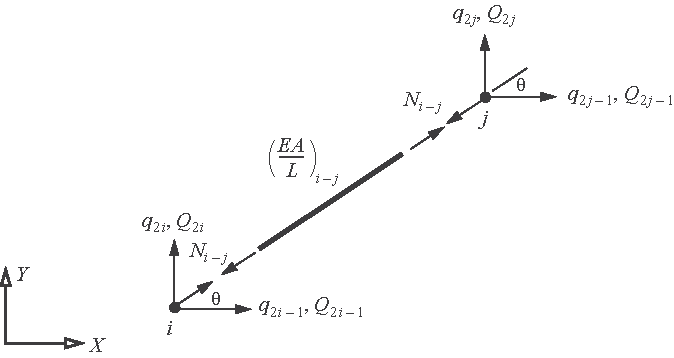
\includegraphics{Figure_16-1.pdf}
}{\caption{Truss bar connected to joints $i$ and~$j$.}\label{fig16.1}}

\vspace*{-1pc}

\noindent The axial force $N_{i-j}$ from eq.~(\ref{eq6.2}) on page \pageref{eq6.2} is
\begin{align}\label{eq16.2}
N_{i-j}=\left(\frac{E A}{L}\right)_{i-j} \Delta_{i\,{-}\,j}-\left(N_{T}\right)_{i\,{-}\,j}.
\end{align}
The elongation $\Delta_{i-j}$ is related to the joint displacements by eq.~(\ref{eq6.6}) on page \pageref{eq6.6}, which is repeated as (\ref{eq16.3}) below.
\begin{align}\label{eq16.3}
\Delta_{i-j}=(\cos \theta)_{i-j}(q_{2 j-1}-q_{2 i-1})+(\sin \theta)_{i-j}(q_{2 j}-q_{2 i}),
\end{align}
In matrix notation (\ref{eq16.3}) is written as
\begin{align}\label{eq16.4}
\Delta_{i-j}=\left[\begin{array}{@{}llll@{}}-c \!\!\!& -s\!\!\! & c\!\!\! & s\end{array}\right]\left[\begin{array}{@{}c@{}}q_{2 i-1} \\q_{2 i} \\q_{2 j} \\q_{2 j-1}\end{array}\right]=[b]^{T}\{q\}_{i-j},
\end{align}
where we introduce the shorthand notation for the trigonometric functions
\begin{align}\label{eq16.5}
c=(\cos \theta)_{i-j} \quad s=(\sin \theta)_{i-j}.
\end{align}
Elements of the 4X1 matrix $[b]$ and the 4X1 displacement vector are
\begin{align}\label{eq16.6}
[b]^{T}=\left[\begin{array}{@{}llll@{}} -c\!\!\! & -s\!\!\! & c\!\!\! & s \end{array}\right] \quad \{q\}_{i-j}^{T}=\left[\begin{array}{@{}llll@{}} q_{2 i-1}\!\!\! & q_{2 i}\!\!\! & q_{2 j-1}\!\!\! & q_{2 j} \end{array}\right].
\end{align}
Substitute the elongation-displacement relation (\ref{eq16.4}) into Hooke's law (\ref{eq16.2}) to get
\begin{align}\label{eq16.7}
N_{i-j}=\left(\frac{E A}{L}\right)_{i-j}[b]^{T}\{q\}_{i-j}-\left(N_{T}\right)_{i-j}.
\end{align}

\vspace*{-1pc}

Free body diagrams of the bar and joints $i$ and $j$ are shown figure~\ref{fig16.1}. External forces in the \textit{X}- and \textit{Y}-directions at joint $i$ are denoted by $Q_{2 i-1}$ and $Q_{2 i}$, respectively, and external forces in the \textit{X}- and \textit{Y}-directions at joint $j$ are denoted by $Q_{2 j-1}$ and $Q_{2 j}$, respectively. Equilibrium at joints $i$ and $j$ yield
\begin{align}\label{eq16.8}
Q_{2 i-1}+N_{i-j} \cos \theta=0, Q_{2 i}+N_{i-j} \sin \theta=0, Q_{2 j-1}-N_{i-j} \cos \theta=0,\mbox{ and }Q_{2 j}-N_{i-j} \sin \theta=0.\hspace*{4pt}
\end{align}
In matrix notation, equilibrium equations (\ref{eq16.8}) are written as
\begin{align}\label{eq16.9}
\left[\begin{array}{@{}c@{}}Q_{2 i-1} \\Q_{2 i} \\Q_{2 j-1} \\Q_{2 j}\end{array}\right]=\left[\begin{array}{@{}c@{}}-c \\-s \\c \\s\end{array}\right] N_{i-j}\mbox{ or }\{Q\}_{i-j}=[b] N_{i-j},
\end{align}
where $\{Q\}_{i-j}$ is the joint force vector and matrix $[b]$ is defined in eq.~(\ref{eq16.6}). Substitute eq.~(\ref{eq16.7}) for the axial force in eq.~(\ref{eq16.9}) to get
\begin{align}\label{eq16.10}
\{Q\}_{i-j}=\left(\frac{E A}{L}\right)_{i-j}[b][b]^{T}\{q\}_{i-j}-[b]\left(N_{T}\right)_{i-j}.
\end{align}
The latter equation is written in the form
\begin{align}\label{eq16.11}
\{Q\}_{i-j}=[K]\{q\}_{i-j}+\left\{Q^{0}\right\}_{i-j},
\end{align}
where $[K]=\left(\frac{E A}{L}\right)_{i-j}[b][b]^{T}$ is the truss stiffness matrix, and $\left\{Q^{0}\right\}_{i-j}=-[b]\left(N_{T}\right)_{i-j}$ is the fixed-end force vector. The stiffness matrix for the truss bar is\pagebreak
\begin{align}\label{eq16.12}
\fbox{$\displaystyle[K]=\left(\frac{E A}{L}\right)_{i-j}\left[\begin{array}{@{}cccc@{}}c^{2} & c s & -c^{2} & -c s \\c s & s^{2} & -c s & -s^{2} \\-c^{2} & -c s & c^{2} & c s \\-c s & -s^{2} & c s & s^{2}\end{array}\right].$}
\end{align}
Properties of the truss stiffness matrix (\ref{eq16.12}):
\begin{itemize}
\item It is symmetric since the bar is linear elastic and the displacements are small.

\item The sum of column elements is zero. This results from equilibrium of the bar for each unit displacement state.

For example UDS 1 $\{q\}=[\begin{array}{@{}llll@{}} 1& 0, & 0 & 0\end{array}]^{T}$ and the joint forces are\\[-3pt]

$\{Q\}=[\begin{array}{@{}llll@{}}Q_{2 i-1} & Q_{2 i} & Q_{2 j-1} & Q_{2 j}\end{array}]^{T}=(E A / L)[\begin{array}{@{}cccc@{}}c^{2} & cs & -c^{2} & -cs\end{array}]^{T}(1)$.\\[-3pt]

Sum forces horizontally $Q_{2 i-1}+Q_{2 j-1}=(E A / L)(c^{2}+(-c^{2}))(1)=0$.

Sum forces vertically $Q_{2 i}+Q_{2 j}=(E A / L)(c s+(-c s))(1)=0$.

Sum moments about joint $i$ $L c Q_{2 j}-L s Q_{2 j-1}=L(E A / L)[c(-c s)-s(-c^{2})](1)=0$.

\item ${Det}[K]=0$ since the bar is not restrained against rigid body displacements.

\item Diagonal elements are positive.
\end{itemize}

The fixed-end force vector is
\begin{align}\label{eq16.13}
\left\{Q^{0}\right\}_{i-j}=\left[\begin{array}{@{}c@{}}Q_{2 i-1}^{0} \\[6pt] Q_{2 i}^{0} \\[6pt]Q_{2 j-1}^{0} \\[6pt]Q_{2 j}^{0}\end{array}\right]=-[b]\left(N_{T}\right)_{i-j}=-\left[\begin{array}{@{}c@{}}-c \\-s \\c \\s\end{array}\right]\left(N_{T}\right)_{i-j}.
\end{align}
Note that the nodal force vector is equal to the fixed-end vector when the joints are fixed and cannot displace; i.e., $\{Q\}_{i-j}=\left\{Q^{0}\right\}_{i-j}$ if $\{q\}^{T}{ }_{i-j}=\left[\begin{array}{@{}llll@{}}0 & 0 & 0 & 0\end{array}\right]$.

Equation (\ref{eq16.7}) is rewritten for bar \textit{i-j} as
\begin{align}\label{eq16.14}
N_{i-j}=[S]\{q\}_{i-j}-\left(N_{T}\right)_{i-j},
\end{align}
where the 1X4 stress matrix $[S]$ is defined as
\begin{align}\label{eq16.15}
[S] \equiv\left(\frac{E A}{L}\right)_{i-j}\left[\begin{array}{@{}llll@{}}-c & -s & c & s\end{array}\right]=\left(\frac{E A}{L}\right)_{i-j}[b]^{T}.
\end{align}

\vspace*{-1pc}

\begin{example}[A three-bar truss]\label{ex16.1}Each bar in the three-bar truss shown in figure~\ref{fig16.2} has the same axial stiffness $EA$, and the joints are numbered as shown. The thermal forces in bar 1-2, 1-3, and 2-3 are denoted by $(N_{T})_{1-2}$, $(N_{T})_{1-3}$, and $(N_{T})_{2-3}$, respectively. Determine the 6X6 unrestrained structural stiffness matrix and the 6X1 fixed-end action vector.

\pagebreak

\processfigure[!h]{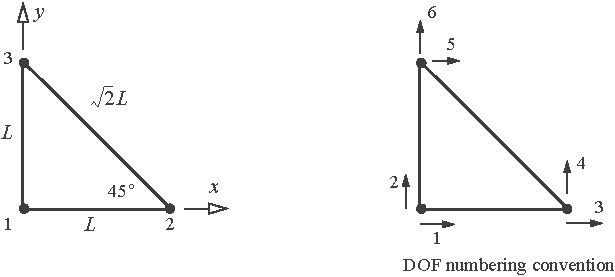
\includegraphics{Figure_16-2.pdf}
}{\caption{Three-bar truss example.}\label{fig16.2}}

\vspace*{-1pc}

\subsubsection{Solution.} The direction cosines and their products for each bar are listed in table~\ref{tab16.1}.

\begin{table}[!h]%Table 16.1
\processtable{Direction cosines for the three-bar truss\label{tab16.1}}
{\tabcolsep=10pt\begin{tabular}{@{}lcccccc@{}}\toprule
\colhead{bar} & \colhead{$\theta$} & \colhead{$c$} & \colhead{$s$} & \colhead{$c^{2}$} & \colhead{$s^{2}$} & \colhead{$cs$}\\\midrule
1--2 & $0^{\circ}$ & 1 & 0 & 1 & 0 & 0\\
1--3 & $90^{\circ}$ & 0 & 1 & 0 & 1 & 0\\
2--3 & $135^{\circ}$ & $-1 / \sqrt{2}$ & $1 / \sqrt{2}$ & $1 / 2$ & $1 / 2$ & $-1 / 2$\\\botrule
\end{tabular}}{}
\vspace*{-1.4pc}
\end{table}

\noindent The direction cosines from table~\ref{tab16.1} are inserted into eqs. (\ref{eq16.12}) and (\ref{eq16.13}), to get the 4X4 stiffness matrices and the 4X1 fixed-end actions for the truss member. The stiffness matrices are expanded to 6X6 by adding two rows and two columns of zeros, and the column vectors are expanded to 6X1 by adding two rows of zeros. Refer to the discussion in article~\ref{sec15.3} on page~\pageref{sec15.3}. The 6X1 vector of forces for bar 1-2 is
\begin{align}\label{eq16.1a}\tag{a}
\left[\begin{array}{@{}l@{}}Q_{1} \\Q_{2} \\Q_{3} \\Q_{4} \\Q_{5} \\Q_{6}\end{array}\right]_{1-2}=\left(\frac{EA}{L}\right)\left[\begin{array}{@{}cccccc@{}}1 & 0 & -1 & 0 & 0 & 0 \\0 & 0 & 0 & 0 & 0 & 0 \\-1 & 0 & 1 & 0 & 0 & 0 \\0 & 0 & 0 & 0 & 0 & 0 \\0 & 0 & 0 & 0 & 0 & 0 \\0 & 0 & 0 & 0 & 0 & 0\end{array}\right]\left[\begin{array}{@{}l@{}}q_{1} \\q_{2} \\q_{3} \\q_{4} \\q_{5} \\q_{6}\end{array}\right]-\left[\begin{array}{@{}c@{}}-1 \\0 \\1 \\0 \\0 \\0\end{array}\right]\left(N_{T}\right)_{1-2}.
\end{align}
Rows five and six, and columns five and six, of the stiffness matrix in eq. (\textbf{\ref{eq16.1a}}) contain zeros entries since degrees of freedom five and six do not influence the response of truss bar 1-2. The 6X1 vector of forces for bar 1-3 is
\begin{align}\label{eq16.1b}\tag{b}
\left[\begin{array}{@{}l@{}}Q_{1} \\Q_{2} \\Q_{3} \\Q_{4} \\Q_{5} \\Q_{6}\end{array}\right]_{1-3} = \left(\frac{EA}{L}\right)\left[\begin{array}{@{}cccccc@{}}0 & 0 & 0 & 0 & 0 & 0 \\0 & 1 & 0 & 0 & 0 & -1 \\0 & 0 & 0 & 0 & 0 & 0 \\0 & 0 & 0 & 0 & 0 & 0 \\0 & 0 & 0 & 0 & 0 & 0 \\0 & -1 & 0 & 0 & 0 & 1\end{array}\right]\left[\begin{array}{@{}c@{}}q_{1} \\q_{2} \\q_{3} \\q_{4} \\q_{5} \\q_{6}\end{array}\right]-\left[\begin{array}{@{}c@{}}0 \\-1 \\0 \\0 \\0 \\1\end{array}\right]\left(N_{T}\right)_{1-3}.
\end{align}
Rows three and four, and columns three and four, of the stiffness matrix in eq. (\textbf{\ref{eq16.1b}}) contain zeros entries since degrees of freedom three and four do not influence the response of truss bar 1-3. The 6X1 vector of\break forces for bar 2-3 is
\begin{align}\label{eq16.1c}\tag{c}
\left[\begin{array}{@{}l@{}}Q_{1} \\Q_{2} \\Q_{3} \\Q_{4} \\Q_{5} \\Q_{6}\end{array}\right]_{2-3} = \left(\frac{EA}{RL}\right)\left[\begin{array}{@{}cccccc@{}}0 & 0 & 0 & 0 & 0 & 0 \\0 & 0 & 0 & 0 & 0 & 0 \\0 & 0 & 1 / 2 & -1 / 2 & -1 / 2 & 1 / 2 \\0 & 0 & -1 / 2 & 1 / 2 & 1 / 2 & -1 / 2 \\0 & 0 & -1 / 2 & 1 / 2 & 1 / 2 & -1 / 2 \\0 & 0 & 1 / 2 & -1 / 2 & -1 / 2 & 1 / 2\end{array}\right]\left[\begin{array}{@{}c@{}}q_{1} \\q_{2} \\q_{3} \\q_{4} \\q_{5} \\q_{6}\end{array}\right]\left[\begin{array}{@{}c@{}}0 \\0 \\1 / \sqrt{2} \\-1 / \sqrt{2} \\-1 / \sqrt{2} \\1 / \sqrt{2}\end{array}\right]\left(N_{T}\right)_{2-3}.
\end{align}
Rows one and two, and columns one and two, of the stiffness matrix in eq. (\textbf{\ref{eq16.1c}}) contain zeros entries since degrees of freedom one and two do not influence the response of truss bar 1-3. Let $a=\frac{1}{2 \sqrt{2}}$, so that
\begin{align}\label{eq16.1d}\tag{d}
\left[\begin{array}{@{}l@{}}Q_{1} \\Q_{2} \\Q_{3} \\Q_{4} \\Q_{5} \\Q_{6}\end{array}\right]_{2-3} = \left(\frac{EA}{L}\right)\left[\begin{array}{@{}cccccc@{}}0 & 0 & 0 & 0 & 0 & 0 \\0 & 0 & 0 & 0 & 0 & 0 \\0 & 0 & a & -a & -a & a \\0 & 0 & -a & a & a & -a \\0 & 0 & -a & a & a & -a \\0 & 0 & a & -a & -a & a\end{array}\right]\left[\begin{array}{@{}l@{}}q_{1} \\q_{2} \\q_{3} \\q_{4} \\q_{5} \\q_{6}\end{array}\right]-\left[\begin{array}{@{}c@{}}0 \\0 \\1 / \sqrt{2} \\-1 / \sqrt{2} \\-1 / \sqrt{2} \\1 / \sqrt{2}\end{array}\right]\left(N_{T}\right)_{2-3}.
\end{align}
Addition of the 6X1 force vectors for each truss member equals the external joint force vector acting on the truss. This addition of force vectors satisfies equilibrium at the joints assuming the procedure to expand each truss element to six degrees of freedom to four degrees of freedom is done correctly. Hence, the condition of equilibrium~is\vspace*{-0.6pc}
\begin{align}\label{eq16.1e}\tag{e}
\left[\begin{array}{@{}l@{}}Q_{1} \\Q_{2} \\Q_{3} \\Q_{4} \\Q_{5} \\Q_{6}\end{array}\right]=\left[\begin{array}{@{}l@{}}Q_{1} \\Q_{2} \\Q_{3} \\Q_{4} \\Q_{5} \\Q_{6}\end{array}\right]_{1-2}+\left[\begin{array}{@{}l@{}}Q_{1} \\Q_{2} \\Q_{3} \\Q_{4} \\Q_{5} \\Q_{6}\end{array}\right]_{1-3}+\left[\begin{array}{@{}l@{}}Q_{1} \\Q_{2} \\Q_{3} \\Q_{4} \\Q_{5} \\Q_{6}\end{array}\right]_{2-3}.
\end{align}
Equations (\textbf{\ref{eq16.1a}}), (\textbf{\ref{eq16.1b}}), and (\textbf{\ref{eq16.1d}}) for the force vectors are substituted into eq. (\textbf{\ref{eq16.1e}}) to get the unrestrained stiffness matrix of the truss as
\begin{align}\label{eq16.1f}\tag{f}
\left[\begin{array}{@{}l@{}}Q_{1} \\Q_{2} \\Q_{3} \\Q_{4} \\Q_{5} \\Q_{6}\end{array}\right]=\frac{E A}{L}\left[\begin{array}{@{}cccccc@{}}1 & 0 & -1 & 0 & 0 & 0 \\0 & 1 & 0 & 0 & 0 & -1 \\-1 & 0 & 1+a & -a & -a & a \\0 & 0 & -a & a & a & -a \\0 & 0 & -a & a & a & -a \\0 & -1 & a & -a & -a & 1+a\end{array}\right]\left[\begin{array}{@{}l@{}}q_{1} \\q_{2} \\q_{3} \\q_{4} \\q_{5} \\q_{6}\end{array}\right]+\left[\begin{array}{@{}c@{}}\left(N_{T}\right)_{1-2} \\\left(N_{T}\right)_{1-3} \\-\left(N_{T}\right)_{1-2}-\left(N_{T}\right)_{2-3} / \sqrt{2} \\\left(N_{T}\right)_{2-3} / \sqrt{2} \\\left(N_{T}\right)_{2-3} / \sqrt{2} \\-\left(N_{T}\right)_{1-3}-\left(N_{T}\right)_{2-3} / \sqrt{2}\end{array}\right].
\end{align}
In compact notation eq. (\textbf{\ref{eq16.1f}}) is
\begin{align}\label{eq16.1g}\tag{g}
\{Q\}=[K]\{q\}+\left\{Q^{0}\right\},
\end{align}
where the 6X6 unrestrained structural stiffness matrix is\pagebreak
\begin{align}\label{eq16.1h}\tag{h}
[K]=\left(\frac{E A}{L}\right)
\begin{array}{@{}c@{}}
{\arraycolsep=7.5pt\begin{array}{@{}cccccc@{}}
q_{1} & q_{2} & q_{3} & q_{4} & q_{5} & q_{6}\end{array}}\\[6pt]
\left[\begin{array}{@{}cccccc@{}}1 & 0 & -1 & 0 & 0 & 0 \\0 & 1 & 0 & 0 & 0 & -1 \\-1 & 0 & 1+a & -a & -a & a \\0 & 0 & -a & a & a & -a \\0 & 0 & -a & a & a & -a \\0 & -1 & a & -a & -a & 1+a\end{array}\right]\end{array},
\end{align}
and the 6X1 fixed-end action vector is
\begin{align}\label{eq16.1i}\tag{i}
\left\{Q^{0}\right\}=\left[\begin{array}{@{}c@{}}\left(N_{T}\right)_{1-2} \\\left(N_{T}\right)_{1-3} \\-\left(N_{T}\right)_{1-2}-\left(N_{T}\right)_{2-3} / \sqrt{2} \\\left(N_{T}\right)_{2-3} / \sqrt{2} \\\left(N_{T}\right)_{2-3} / \sqrt{2} \\-\left(N_{T}\right)_{1-3}-\left(N_{T}\right)_{2-3} / \sqrt{2}\end{array}\right].
\end{align}
Note that the stiffness matrix in eq. (\textbf{\ref{eq16.1h}}) is symmetric; the sum of column elements equals zero; diagonal elements are positive; and its determinate vanishes.
\end{example}

\vspace*{-1pc}

\subsection{Assembly algorithm}\label{sec16.1.1}

Consider again the three-bar truss in example~\ref{ex16.1} on page \pageref{ex16.1}. For computer implementation an algorithm is presented to assemble the 6X6 unrestrained structural stiffness matrix from the three 4X4 truss stiffness matrices, and to assemble the 6X1 fixed-end vector from the three 4X1 fixed-end action vectors. Let a truss member be denoted by $m$, where $m = 1$ for bar 1-2, $m = 2$ for bar 1-3, and $m = 3$ for bar 2-3. A description of symbols used in the of assembly algorithm is given in table~\ref{tab16.2}.

%Table 16.2
\begin{table}[!h]
\processtable{Nomenclature\label{tab16.2}}
{\tabcolsep=10pt\begin{tabular}{@{}ll@{}}\toprule
\colhead{Symbol} & \colhead{Description}\\\midrule
$[K]$ & 6X6 unrestrained stiffness matrix\\
$K({row, col })$ & row and column elements of the unrestrained stiffness matrix\\
$[K_{m}]$ & 4X4 stiffness matrix for truss member $m$\\
$K_{m}(i, j)$ & matrix elements of the truss member stiffness matrix\\
$\{Q^{0}\}$ & 6X1 fixed-end action vector\\
$Q^{0}({row})$ & row elements of the fixed-end action vector\\
$\{Q_{m}^{(0)}\}$ & 4X1 fixed-end action vector of truss member $m$\\
$Q_{m}^{0}(i)$ & row elements of the truss member fixed-end action vector\\\botrule
\end{tabular}}{}
\vspace*{-1pc}
\end{table}

Define the 3X1 ``spring'' stiffness vector $[K_{t}]$ and the 3X1 thermal force vector $[N T]$ by
\begin{align}\label{eq16.16}
[K t]=\left[\frac{E A}{L} \frac{E A}{L} \frac{E A}{\sqrt{2} L}\right]^{T} \quad[N T]=\left[\left(N_{T}\right)_{1-2}\left(N_{T}\right)_{1-3}\left(N_{T}\right)_{2-3}\right]^{T}.
\end{align}
Direction cosines for each truss bar are specified in the 4X1 matrices $\left[b_{i}\right]$, $i=1,2,3$, in eq.~(\ref{eq16.17}) below:\pagebreak
\begin{align}\label{eq16.17}
\left[b_{1}\right]=\left[\begin{array}{@{}llll@{}}-1 & 0 & 1 & 0\end{array}\right]^{T} \quad\left[b_{2}\right]=\left[\begin{array}{@{}llll@{}}0 & -1 & 0 & 1\end{array}\right]^{T} \quad\left[b_{3}\right]=\left[\frac{1}{\sqrt{2}}-\frac{1}{\sqrt{2}}-\frac{1}{\sqrt{2}} \frac{1}{\sqrt{2}}\right]^{T}.
\end{align}
Defined a 3X4 \textbf{connectivity matrix} $[C]$ by\vspace*{-0.6pc}
\begin{align}\label{eq16.18}
&\hspace*{2.5pc}q_{2 i-1} \hspace*{1.2pc} q_{2 i} \hspace*{1.2pc} q_{2 j-1} \hspace*{1.2pc} q_{2 j} \nonumber\\
&[C]=
%\begin{array}{@{}c@{}}
%{%\arraycolsep=5pt
%\hskip-65pt\begin{array}{@{\hspace*{-9pt}}ccc@{\hspace*{14pt}}c@{}}
%q_{2 i-1} & q_{2 i} & q_{2 j-1} & q_{2 j}\end{array}}\\[6pt]
{\arraycolsep=13.5pt\left[\begin{array}{@{\hspace*{6pt}}cccc@{\hspace*{6pt}}}
%q_{2 i-1} & q_{2 i} & q_{2 j-1} & q_{2 j} \\
1 & 2 & 3 & 4 \\
1 & 2 & 5 & 6 \\
3 & 4 & 5 & 6\end{array}\right]} \quad \begin{array}{l}\text {member 1 } \\\text {member 2}\ . \\\text {member 3 }\end{array}
%\end{array}
\end{align}

\vspace*{-1.6pc}

\noindent Row one of matrix $[C]$ is assigned to member 1 (bar 1-2), row two to member 2 (bar 1-3), and row three to member 3 (bar 2-3).\vspace*{-2pt}

\processfigure[!b]{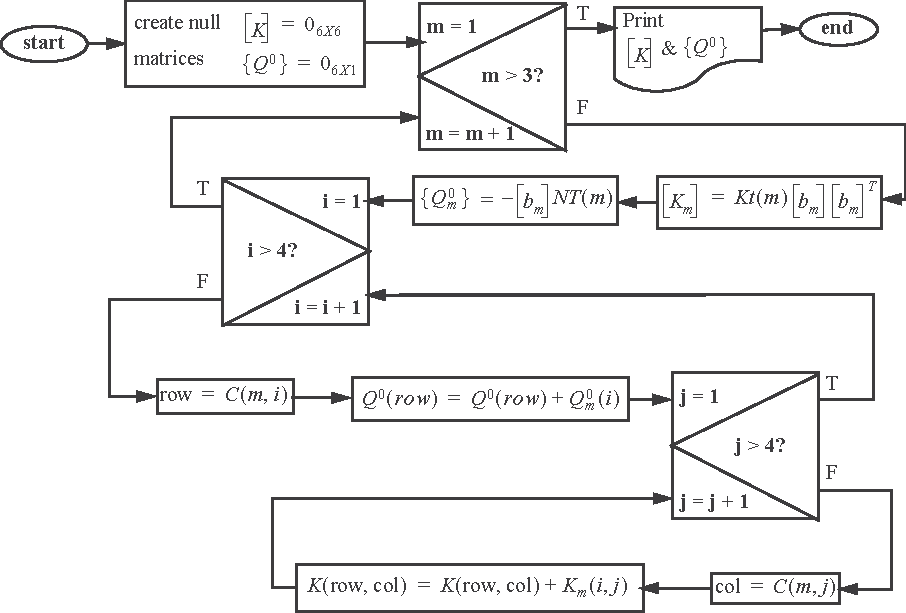
\includegraphics{Figure_16-3.pdf}
}{\caption{Flow chart of the assembly algorithm.}\label{fig16.3}}

\begin{unlist}
\item Column one contains the DOF for horizontal displacement $q_{2 i-1}$ at the beginning joint $i$ of the member,
\item column two contains the DOF for the vertical displacement $q_{2 i}$ of the beginning joint \textit{i} of the member,
\item column three contains the DOF of the horizontal displacement $q_{2 j-1}$ at the end joint $j$ of the member,
\item and column four contains the DOF for the vertical displacement $q_{2 j}$ at the end joint $j$ of the member.
\end{unlist}

Refer to the nomenclature in table~\ref{tab16.2}, and to matrices defined in eqs. (\ref{eq16.16}), (\ref{eq16.17}), and (\ref{eq16.18}), to understand the flow chart for the assembly algorithm in figure~\ref{fig16.3}.

\pagebreak

\begin{example}[Restrained three-bar truss of example~\ref{ex16.1}]\label{ex16.2}Consider the truss of example~\ref{ex16.1} supported in such a manner that joint displacements $q_{1}=q_{2}=q_{4}=q_{5}=0$ as is shown in figure~\ref{fig16.4}. The unknown displacements are $q_3$ and $q_6$, and take the corresponding joint forces $Q_{3}=Q_{6}=0$. The thermal forces in bars 1-2, 1-3, and 2-3 are specified as $\left(N_{T}\right)_{1-2}=0$, $\left(N_{T}\right)_{1-3} \neq 0$, and $\left(N_{T}\right)_{2-3}=0$, respectively.

\processfigure[!h]{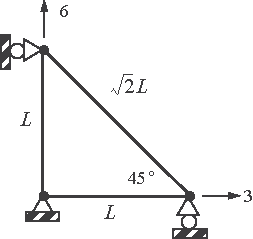
\includegraphics{Figure_16-4.pdf}
}{\caption{Statically indeterminate three-bar truss.}\label{fig16.4}}


\begin{enumerate}
\item[a)] Determine the restrained structural stiffness matrix $\left[K_{\alpha \alpha}\right]$, and submatrices $\left[K_{\alpha \beta}\right]$, $\left[K_{\beta \alpha}\right]$, and $\left[K_{\beta \beta}\right]$.

\item[b)] Determine the unknown joint displacements $q_{3}$, and $q_{6}$.

\item[c)] Determine the unknown support reactions $Q_{1}, Q_{2}, Q_{4}$, and $Q_{5}$.

\item[d)] Determine the bar forces $N_{1-2}, N_{1-3}$, and $N_{2-3}$.
\end{enumerate}

\subsubsection{Solution to part (a).} Rearrange the unrestrained stiffness matrix in eq. (\textbf{\ref{eq16.1h}}) of example~\ref{ex16.1} so that the order of the rows and columns correspond to degrees of freedom 3, 6, 1, 2, 4, and 5.
\begin{align}\label{eq16.2a}\tag{a}
[K]=\left(\frac{E A}{L}\right)
\begin{array}{@{}c@{}}
{\arraycolsep=7.5pt\begin{array}{@{}cccccc@{}}
q_3 & q_6 & q_1 & q_2 & q_4 & q_5
\end{array}}\\[6pt]
\left[\begin{array}{cc;{2pt/2pt}cccc}
1+a & a & -1 & 0 & -a & -a \\
a & 1+a & 0 & -1 & -a & -a \\\hdashline[2pt/2pt]
-1 & 0 & 1 & 0 & 0 & 0 \\ 0 & -1 & 0 & 1 & 0 & 0 \\ -a & -a & 0 & 0 & a & a \\ -a & -a & 0 & 0 & a & a\end{array}\right]\end{array}.
\end{align}
Compare the matrix in eq. (\textbf{\ref{eq16.2a}}) to the general form (\ref{eq15.27}) on page \pageref{eq15.27} to identify
\begin{align}\label{eq16.2b}\tag{b}
\left[K_{\alpha \alpha}\right]=\left(\frac{E A}{L}\right)\left[\begin{array}{@{}cc@{}}1+a & a \\a & 1+a\end{array}\right] \quad\left[K_{\alpha \beta}\right]=\left(\frac{E A}{L}\right)\left[\begin{array}{@{}cccc@{}}-1 & 0 & -a & -a \\0 & -1 & -a & -a\end{array}\right],
\end{align}
and
\begin{align}\label{eq16.2c}\tag{c}
\left[K_{\beta \alpha}\right]=\left(\frac{E A}{L}\right)\left[\begin{array}{@{}cc@{}}-1 & 0 \\0 & -1 \\-a & -a \\-a & -a\end{array}\right] \quad\left[K_{\beta \beta}\right]=\left(\frac{E A}{L}\right)\left[\begin{array}{@{}llll@{}}1 & 0 & 0 & 0 \\0 & 1 & 0 & 0 \\0 & 0 & a & a \\0 & 0 & a & a\end{array}\right].
\end{align}
The restrained structural stiffness matrix $[K_{\alpha \alpha}]$ is symmetric, and the sum of its column elements is not zero. Also note that the restrained stiffness structural matrix can be obtained from the unrestrained structural stiffness matrix in eq.~(\textbf{\ref{eq16.2h}}) by merely crossing out rows and columns 1, 2, 4, and 5:
\begin{align}\label{eq16.2d}\tag{d}
[K]=\left(\frac{E A}{L}\right)
\begin{array}{@{}c@{}}
{\arraycolsep=7.5pt\begin{array}{@{}cccccc@{}}
q_1 & q_2 & q_3 & q_4 & q_5 & q_6
\end{array}}\\[6pt]
\left[\begin{array}{@{}cccccc@{}} \multirow{6}{2pt}{\hspace*{3pt}\rule{0.5pt}{76pt}}\hspace*{-1pt}1 & \multirow{6}{2pt}{\hspace*{3pt}\rule{0.5pt}{76pt}}\hspace*{-1pt}0 & -1 & \multirow{6}{2pt}{\hspace*{3pt}\rule{0.5pt}{76pt}}\hspace*{-1pt}0 & \multirow{6}{2pt}{\hspace*{3pt}\rule{0.5pt}{76pt}}\hspace*{-1pt}0 & 0 \\[-7pt]
\hline\\[-4pt] 0 & 1 & 0 & 0 & 0 & -1 \\[-7pt]
\hline\\[-4pt] -1 & 0 & 1+a & -a & -a & a \\
0 & 0 & -a & a & a & -a \\[-7pt]
\hline\\[-4pt]
0 & 0 & -a & a & a & -a \\[-7pt]
\hline\\[-4pt] 0 & -1 & a & -a & -a & 1+a\end{array}\right]\end{array}.
\end{align}%\stop
The fixed-end action vector in eq. (\textbf{\ref{eq16.1i}}) of example \ref{ex16.1} for the unrestrained truss reduces to
\begin{align}\label{eq16.2e}\tag{e}
\left\{Q^{0}\right\}=\left[\begin{array}{@{}llllll@{}}0 & \left(N_{T}\right)_{1-3} & 0 & 0 & 0 & -\left(N_{T}\right)_{1-3}\end{array}\right]^{T}.
\end{align}
Elements in rows 3 and 6 constitute $\left\{Q_{\alpha}^{0}\right\}$ while the remaining rows constitute $\left\{Q_{\beta}^{0}\right\}$. Thus,
\begin{align}\label{eq16.2f}\tag{f}
\left\{Q_{\alpha}^{0}\right\}=\left[\begin{array}{@{}c@{}}0 \\-\left(N_{T}\right)_{1-3}\end{array}\right] \quad\left\{Q_{\beta}^{0}\right\}=\left[\begin{array}{@{}c@{}}0 \\\left(N_{T}\right)_{1-3} \\0 \\0\end{array}\right].
\end{align}

\vspace*{-1pc}

\subsubsection{Solution to part (b).} Equation (\ref{eq15.31}) on page \pageref{eq15.31} with the addition of the fixed-end action vector is
\begin{align}\label{eq16.2g}\tag{g}
\left\{Q_{\alpha}\right\}=\left[K_{\alpha \alpha}\right]\left\{q_{\alpha}\right\}+\left[K_{\alpha \beta}\right]\left\{q_{\beta}\right\}+\left\{Q_{\alpha}^{0}\right\}.
\end{align}
The fixed-end action vector is subtracted from each side of this equation, since it is a known vector determined from the specified temperature changes in the bars. That is, eq. (\textbf{\ref{eq16.2g}}) is written in the form
\begin{align}\label{eq16.2h}\tag{h}
\left\{Q_{\alpha}\right\}+\underbrace{(-\{Q_{\alpha}^{0}\})}_{\hspace*{-11pc}\mbox{equivalent joint force vector---}}=\left[K_{\alpha \alpha}\right]\left\{q_{\alpha}\right\}+\left[K_{\alpha \beta}\right]\left\{q_{\beta}\right\}.
\end{align}
The vector $-\left\{Q^{0}\right\}$ is called the \textbf{equivalent joint force vector}. In this example the prescribed joint displacement vector is $\left\{q_{\beta}\right\}=\left[\begin{array}{@{}llll@{}}q_{1} & q_{2} & q_{4} & q_{5}\end{array}\right]^{T}=\left[\begin{array}{@{}llll@{}}0 & 0 & 0 & 0\end{array}\right]^{T}$, and the prescribed joint force vector is $\left\{Q_{\alpha}\right\}^{T}=\left[\begin{array}{@{}ll@{}}Q_{3} & Q_{6}\end{array}\right]=\left[\begin{array}{@{}ll@{}}0 & 0\end{array}\right]$. The solution for the unknown joint displacement vector is
\begin{align}\label{eq16.2i}\tag{i}
\left\{q_{\alpha}\right\}=\left[K_{\alpha \alpha}\right]^{-1}\left\{-Q_{\alpha}^{0}\right\}\mbox{, where the inverse matrix is }\left[K_{\alpha \alpha}\right]^{-1}=\left(a d j\left[K_{\alpha \alpha}\right]\right) /\left({det}\left[K_{\alpha \alpha}\right]\right).
\end{align}
The adjoint of the restrained structural stiffness matrix and its determinate are\footnote{The $det([A])$, where $k$ is a scalar and $[A]$ is an $n$-by-$n$ matrix, is equal to $k^n det[A]$.}
\begin{align}\label{eq16.2j}\tag{j}
a d j\left[K_{\alpha \alpha}\right]=\left(\frac{E A}{L}\right)\left[\begin{array}{@{}cc@{}}1+a & -a \\-a & 1+a\end{array}\right] \quad {det}\left[K_{\alpha \alpha}\right]=\left(\frac{E A}{L}\right)^{2}\left((1+a)^{2}-a^{2}\right)=\left(\frac{E A}{L}\right)^{2}(1+2 a).
\end{align}
So the inverse of the restrained structural stiffness matrix is
\begin{align}\label{eq16.2k}\tag{k}
\left[K_{\alpha \alpha}\right]^{-1}=\left(\frac{L}{E A}\right)\left(\frac{1}{1+2 a}\right)\left[\begin{array}{@{}cc@{}}1+a & -a \\-a & 1+a\end{array}\right].
\end{align}
Perform a check of this inverse. Is $\left[K_{\alpha \alpha}\right]\left[K_{\alpha \alpha}\right]^{-1}=[I]$?
\begin{align}
\left(\frac{E A}{L}\right)&\left[\begin{array}{@{}cc@{}}1+a & a \\a & 1+a\end{array}\right]\left(\frac{L}{E A}\right)\left(\frac{1}{1+2 a}\right)\left[\begin{array}{@{}cc@{}}1+a & -a \\-a & 1+a\end{array}\right]=\left(\frac{1}{1+2 a}\right)\left[\begin{array}{@{}cc@{}}1+a & a \\a & 1+a\end{array}\right]\left[\begin{array}{@{}cc@{}}1+a & -a \\-a & 1+a\end{array}\right] \nonumber\\
&=\frac{1}{1+2 a}\left[\begin{array}{@{}cc@{}}(1+a)^{2}+\left(-a^{2}\right) &(1+a)(-a)+a(1+a) \\ a(1+a)+(1+a)(-a)&-a^{2}+(1+a)^2\end{array}\right]=\frac{1}{1+2 a}\left[\begin{array}{@{}cc@{}}1+2 a & 0 \\0 & 1+2 a\end{array}\right]=\left[\begin{array}{@{}cc@{}}1 & 0 \\0 & 1\end{array}\right].\label{eq16.2l}\tag{l}
\end{align}
Hence, the inverse satisfies $\left[K_{\alpha \alpha}\right]\left[K_{\alpha \alpha}\right]^{-1}=[I]$. The solution for the unknown nodal displacement vector is
\begin{align}\label{eq16.2m}\tag{m}
\left[\begin{array}{@{}l@{}}q_{3} \\q_{6}\end{array}\right]=\left(\frac{L}{E A}\right)\left[\begin{array}{@{}l@{}}\frac{-\sqrt{2}}{4+2 \sqrt{2}} \\[6pt]\frac{4+\sqrt{2}}{4+2 \sqrt{2}}\end{array}\right]\left(N_{T}\right)_{1-3}.
\end{align}

\vspace*{-1pc}

\subsubsection{Solution to part (c).} The support reactions are determined from eq.~(\ref{eq15.32}) on page \pageref{eq15.32}, which is repeated below as eq. (\textbf{\ref{eq16.2n}}).
\begin{align}\label{eq16.2n}\tag{n}
\left\{Q_{\beta}\right\}=\left[K_{\beta \alpha}\right]\left\{q_{\alpha}\right\}+\left[K_{\beta \beta}\right]\left\{q_{\beta}\right\}+\left\{Q_{\beta}^{0}\right\}.
\end{align}
\noindent The prescribed joint displacement vector $\left\{q_{\beta}\right\}=0_{4 X 1}$, and submatrix $\left[K_{\beta \alpha}\right]$ was determined in part (\textbf{\ref{eq16.2a}}). Hence,
\begin{align}\label{eq16.2o}\tag{o}
\left[\begin{array}{@{}l@{}}Q_{1} \\Q_{2} \\Q_{4} \\Q_{5}\end{array}\right]=\left(\frac{E A}{L}\right)\left[\begin{array}{@{}cc@{}}-1 & 0 \\0 & -1 \\-a & -a \\-a & -a\end{array}\right]\left[\begin{array}{@{}l@{}}q_{3} \\q_{6}\end{array}\right]+\left[\begin{array}{@{}c@{}}0 \\\left(N_{T}\right)_{1-3} \\0 \\0\end{array}\right].
\end{align}
Substitute eq. (\textbf{\ref{eq16.2m}}) for the displacement vector into eq. (\textbf{\ref{eq16.2o}}) to get
\begin{align}\label{eq16.2p}\tag{p}
\left[\begin{array}{@{}l@{}}Q_{1} \\Q_{2} \\Q_{4} \\Q_{5}\end{array}\right]=\left(\frac{E A}{L}\right)\left[\begin{array}{@{}cc@{}}
-1 & 0 \\0 & -1 \\-a & -a \\-a & -a\end{array}\right]\left(\frac{L}{E A}\right)\left[\begin{array}{@{}c@{}}\frac{-1}{2\,+\,2 \sqrt{2}} \\[6pt]\frac{4\,+\,\sqrt{2}}{4\,+\,2 \sqrt{2}}\end{array}\right]\left(N_{T}\right)_{1-3}+\left[\begin{array}{@{}c@{}}0 \\\left(N_{T}\right)_{1-3} \\0 \\0\end{array}\right].
\end{align}
\noindent After matrix algebra the reactive joint forces are
\begin{align}\label{eq16.2q}\tag{q}
\left[\begin{array}{@{}l@{}}Q_{1} \\Q_{2} \\Q_{4} \\Q_{5}\end{array}\right]=\left[\begin{array}{@{}c@{}}\frac{1}{2\,+\,2 \sqrt{2}} \\[6pt]\frac{1}{2\,+\,2 \sqrt{2}} \\[6pt]\frac{1}{2}-\frac{1}{\sqrt{2}} \\[6pt]\frac{1}{2}-\frac{1}{\sqrt{2}}\end{array}\right]\left(N_{T}\right)_{1-3}.
\end{align}
A free body diagram of all the joint forces is shown in figure~\ref{fig16.5}.

The condition for horizontal equilibrium is $Q_{1}+Q_{5}=0$. Substitute the results for these reactive forces from eq. (\textbf{\ref{eq16.2q}}) into condition for horizontal equilibrium to get
\begin{align}\label{eq16.2r}\tag{r}
Q_{1}+Q_{5}=\left(\frac{1}{2+2 \sqrt{2}}+\frac{1}{2}-\frac{1}{\sqrt{2}}\right)\left(N_{T}\right)_{1-3}.
\end{align}

\pagebreak

\begin{wrapfigure}[12]{L}{132pt}
%\vspace{-19pt}
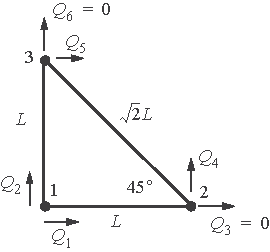
\includegraphics{Figure_16-5.pdf}
\caption{Joint forces acting on the truss. \label{fig16.5}}
\vspace*{-1pc}
\end{wrapfigure}

\noindent Extract a common denominator in eq. (\textbf{\ref{eq16.2r}}):
\begin{align}\label{eq16.2s}\tag{s}
Q_{1}+Q_{5}=\left(\frac{1}{2+2 \sqrt{2}}\right)\left[1+(1+\sqrt{2})-\frac{(2+2 \sqrt{2})}{\sqrt{2}}\right]\left(N_{T}\right)_{1-3}.
\end{align}
Combine terms in eq. (\textbf{\ref{eq16.2s}}) to get the final result
\begin{align}
Q_{1}+Q_{5}&=\left(\frac{1}{2+2 \sqrt{2}}\right)[2+\sqrt{2}-(\sqrt{2}+2)]\left(N_{T}\right)_{1-3}=\left(\frac{1}{2+2 \sqrt{2}}\right)[0]\left(N_{T}\right)_{1-3} \nonumber\\
&=0. \label{eq16.2t}\tag{t}
\end{align}
Hence, the matrix solution for reactive forces $Q_1$ and $Q_5$ satisfy horizontal equilibrium. The condition for vertical equilibrium is $Q_{2}+Q_{4}=0$. Substitute the results for these reactive forces from eq. (\textbf{\ref{eq16.2q}}) into the condition for vertical equilibrium to get
\begin{align}\label{eq16.2u}\tag{u}
Q_{2}+Q_{4}=\left[\frac{1}{2+2 \sqrt{2}}+\frac{1}{2}-\frac{1}{\sqrt{2}}\right]\left(N_{T}\right)_{1-3}=0.
\end{align}
Note that the algebra in eq. (\textbf{\ref{eq16.2u}}) is the same as the algebra detailed in eq. (\textbf{\ref{eq16.2r}}) to eq. (\textbf{\ref{eq16.2t}}). So the condition for vertical equilibrium is satisfied. Vanishing of the moment about joint 1 requires $L Q_{4}-L Q_{5}=0$. Substitute the results for these reactive forces from eq. (\textbf{\ref{eq16.2q}}) into the condition for moment equilibrium to get
\begin{align}\label{eq16.2v}\tag{v}
L Q_{4}-L Q_{5}=L\left[\frac{1}{2}-\frac{1}{\sqrt{2}}-\left(\frac{1}{2}-\frac{1}{\sqrt{2}}\right)\right]\left(N_{T}\right)_{1-3}=0.
\end{align}
Hence, the matrix solution for the reactive forces plus the applied forces satisfies equilibrium of the free body diagram for the entire truss.

\subsubsection{Solution to part (d).} The axial normal force in the bar between joints $i$ and $j$ from eq.~(\ref{eq16.14}) is
\begin{align}\label{eq16.2w}\tag{w}
N_{i-j}=\left[S_{i-j}\right]\{q\}_{i-j}-\left(N_{T}\right)_{i-j},
\end{align}
where the stress matrix (\ref{eq16.15}) is
\begin{align}\label{eq16.2x}\tag{x}
\left[S_{i-j}\right] \equiv\left(\frac{E A}{L}\right)_{i-j}\left[\begin{array}{@{}l@{\;}l@{\;}l@{\;}l@{}}-c & -s & c & s\end{array}\right]_{i-j}.
\end{align}
The direction cosines for each bar are listed in table~\ref{tab16.1}.

For bar 1-2, the axial normal force is
\begin{align}\label{eq16.2y}\tag{y}
N_{1-2}=\left(\frac{E A}{L}\right)\left[\begin{array}{@{}l@{\;}l@{\;}l@{\;}l@{}}-1 & 0 & 1 & 0\end{array}\right]\left[\begin{array}{@{}l@{}}q_{1} \\q_{2} \\q_{3} \\q_{4}\end{array}\right]-\left(N_{T}\right)_{1-2}=\left(\frac{E A}{L}\right)\left[\begin{array}{@{}l@{\;}l@{\;}l@{\;}l@{}}-1 & 0 & 1 & 0\end{array}\right]\left[\begin{array}{@{}c@{}}0 \\0 \\q_{3} \\0\end{array}\right]-0=\left(\frac{E A}{L}\right) q_{3}.
\end{align}
From eq. (\textbf{\ref{eq16.2m}}) the solution for the displacement is $q_{3}=\left(\frac{L}{E A}\right)\left(\frac{-\sqrt{2}}{4\,{+}\,2 \sqrt{2}}\right)\left(N_{T}\right)_{1-3}$, Substitute the result for $q_3$ into eq. (\textbf{\ref{eq16.2y}}) to find
\begin{align*}
N_{1-2}=\left(\frac{E A}{L}\right)\left(\frac{L}{E A}\right)\left(\frac{-\sqrt{2}}{4+2 \sqrt{2}}\right)\left(N_{T}\right)_{1-3}=\left(\frac{-\sqrt{2}}{4+2 \sqrt{2}}\right)\left(N_{T}\right)_{1-3}.
\end{align*}
For bar 1-3, the axial normal force is
\begin{align}\label{eq16.2z}\tag{z}
N_{1-3}=\left(\frac{E A}{L}\right)\left[\begin{array}{@{}l@{\;}l@{\;}l@{\;}l@{}}0 & -1 & 0 & 1\end{array}\right]\left[\begin{array}{@{}c@{}}0 \\0 \\0 \\q_{6}\end{array}\right]-\left(N_{T}\right)_{1-3}=\left(\frac{E A}{L}\right) q_{6}-\left(N_{T}\right)_{1-3}.
\end{align}
From eq. (\textbf{\ref{eq16.2m}}) the solution for the displacement is $q_{6}=\left(\frac{L}{E A}\right) \frac{4+\sqrt{2}}{4\,{+}\,2 \sqrt{2}}\left(N_{T}\right)_{1-3}$. Substitute the result for $q_6$ into eq. (\textbf{\ref{eq16.2z}}) to find
\begin{align}\label{eq16.2aa}\tag{aa}
N_{1-3}=\left(\frac{E A}{L}\right)\left[\left(\frac{L}{E A}\right) \frac{4+\sqrt{2}}{4+2 \sqrt{2}}\left(N_{T}\right)_{1-3}\right]-\left(N_{T}\right)_{1-3}=\left(\frac{-1}{2+2 \sqrt{2}}\right)\left(N_{T}\right)_{1-3}.
\end{align}
For bar 2-3, the axial normal force is\vspace*{-3pt}
\begin{align}\label{eq16.2ab}\tag{ab}
N_{2-3}=\left(\frac{E A}{\sqrt{2} L}\right)\left[\begin{array}{@{}lll@{}}1 / \sqrt{2}-1 / \sqrt{2}-1 / \sqrt{2}\  1\; /\; \sqrt{2}\end{array}\hspace*{-3pt}\right]\left[\begin{array}{@{}l@{}}q_{3} \\
q_{4} \\q_{5} \\q_{6}\end{array}\right]-\left(N_{T}\right)_{2-3}=\left(\frac{E A}{\sqrt{2} L}\right)\left[\begin{array}{@{}lll@{}}1 / \sqrt{2}-1 / \sqrt{2}-1 / \sqrt{2}\  1 / \sqrt{2}\end{array}\hspace*{-3pt}\right]\left[\begin{array}{@{}c@{}}q_{3} \\0 \\0 \\q_{6}\end{array}\right]-0.
\end{align}
Expand eq. (\textbf{\ref{eq16.2ab}}) to get
\begin{align}
N_{2-3}&=\left(\frac{E A}{2 L}\right)\left[\begin{array}{@{}l@{\;}l@{}}1 & 1\end{array}\right]\left[\begin{array}{@{}l@{}}q_{3} \\q_{6}\end{array}\right]-\left(N_{T}\right)_{2-3}=\frac{E A}{2 L}\left(q_{3}+q_{6}\right)-0 \nonumber\\
&=\frac{E A}{2 L}\left[\left(\frac{L}{E A}\right)\left(\frac{-\sqrt{2}}{4+2 \sqrt{2}}\right)\left(N_{T}\right)_{1-3}+\left(\frac{L}{E A}\right) \frac{4+\sqrt{2}}{4+2 \sqrt{2}}\left(N_{T}\right)_{1-3}\right] \nonumber\\
&=\left(\frac{1}{2}\right)\left[\frac{-\sqrt{2}}{4+2 \sqrt{2}}+\frac{4+\sqrt{2}}{4+2 \sqrt{2}}\right]\left(N_{T}\right)_{1-3}=\left(\frac{1}{2}\right)\left[\frac{4}{4+2 \sqrt{2}}\right]\left(N_{T}\right)_{1-3}.\label{eq16.2ac}\tag{ac}
\end{align}
The final result for the force in bar 2-3 is
\begin{align}\label{eq16.2ad}\tag{ad}
N_{2-3}=\frac{\left(N_{T}\right)_{1-3}}{2+\sqrt{2}}.
\end{align}
Note that for this statically indeterminate truss all three bar forces are proportional to the change in temperature of bar 1-3.
\end{example}



\subsection{Self-strained truss}\label{sec16.1.2}

Strain of the bars in a truss can occur due to temperature changes and also due to the \textbf{lack of fit} during assembly, even in the absence of applied nodal forces. The analysis for lack of fit of bar 1-3 in example~\ref{ex16.2} is achieved by replacing the thermal force by
\begin{align*}
\left(N_{T}\right)_{1-3} \rightarrow E A(\overline{\Delta} / L)_{1-3},
\end{align*}
where $\overline{\Delta}$ is the specified displacement of the bar to connect it to joints 1 and 3. For a gap between joints $\overline{\Delta}>0$ and for an overlap $\overline{\Delta}<0$. Hence, the solution for the bar forces in example~\ref{ex16.2} can be interpreted for the problem of lack of fit of bar 1-3 by replacing $\left(N_{T}\right)_{1-3}$ with $E A(\overline{\Delta}/ L)_{1-3}$.

\pagebreak

\begin{example}[Self-strained configuration of the truss in example \ref{ex16.2}]\label{ex16.3}Now consider a statically determinate configuration of the truss in figure~\ref{fig16.2}, which is shown in figure~\ref{fig16.6}. Support conditions impose displacements $q_{2}=q_{4}=q_{5}=0$. The applied external forces are specified as $Q_{1}=Q_{3}=Q_{6}=0$, and only bar 1-3 is subject to a thermal force $\left(N_{T}\right)_{1-3}=E A(\alpha \Delta T)$.
\begin{enumerate}
\item[a)] Determine the unknown joint displacements.

\item[b)] Determine the unknown joint forces.

\item[c)] Determine the elongation of each bar.
\end{enumerate}

\processfigure[!h]{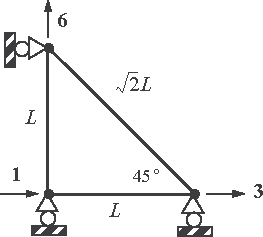
\includegraphics{Figure_16-6.pdf}
}{\caption{Statically determinate three-bar truss.}\label{fig16.6}}

\subsubsection{Solution to part (a).} The matrix equation to determine the unknown joint displacements is
\begin{align}\label{eq16.3a}\tag{a}
\left\{Q_{\alpha}\right\}=\left[K_{\alpha \alpha}\right]\left\{q_{\alpha}\right\}+\left[K_{\alpha \beta}\right]\left\{q_{\beta}\right\}+\left\{Q_{\alpha}^{0}\right\}.
\end{align}
Refer to the stiffness matrix in eq. (\textbf{\ref{eq16.3h}}) and the fixed-end vector in eq. (\textbf{\ref{eq16.1i}}) of example \ref{ex16.1}. Then the matrices in eq. (\textbf{\ref{eq16.3a}}) are
\begin{gather}
\left\{Q_{\alpha}\right\}=\left[\begin{array}{@{}c@{}}Q_{1} \\Q_{3} \\Q_{6}\end{array}\right]=\left[\begin{array}{@{}l@{}}0 \\0 \\0\end{array}\right], \left[K_{\alpha \alpha}\right]=\frac{E A}{L}\left[\begin{array}{@{}ccc@{}}1 & -1 & 0 \\-1 & 1+a & a \\0 & a & 1+a\end{array}\right], \left\{q_{\alpha}\right\}=\left[\begin{array}{@{}l@{}}q_{1} \\q_{3} \\q_{6}\end{array}\right], \left[K_{\alpha \beta}\right]=\frac{E A}{L}\left[\begin{array}{@{}ccc@{}}0 & 0 & 0 \\0 & -a & -a \\-1 & -a & -a\end{array}\right],\label{eq16.3b}\tag{b}\\
\left\{q_{\beta}\right\}=\left[\begin{array}{@{}l@{}}q_{2} \\q_{4} \\q_{5}\end{array}\right]=\left[\begin{array}{@{}l@{}}0 \\0 \\0\end{array}\right]\mbox{, and }\left\{Q_{\alpha}^{0}\right\}=\left[\begin{array}{r}Q_{1}^{0} \\[6pt] Q_{3}^{0} \\[6pt] Q_{6}^{0}\end{array}\right]=\left[\begin{array}{@{}c@{}}0 \\0 \\-\left(N_{T}\right)_{1-3}\end{array}\right].\label{eq16.3c}\tag{c}
\end{gather}
The solution to eq. (\textbf{\ref{eq16.3a}}) for the joint displacements is
\begin{align}\label{eq16.3d}\tag{d}
q_{1}=-L(\alpha \Delta T) \quad q_{3}=-L(\alpha \Delta T) \quad q_{6}=L(\alpha \Delta T).
\end{align}

\vspace*{-1pc}

\subsubsection{Solution to part (b).} The matrix equation to determine the unknown joint forces is
\begin{align}\label{eq16.3e}\tag{e}
\left\{Q_{\beta}\right\}=\left[K_{\beta \alpha}\right]\left\{q_{\alpha}\right\}+\left[K_{\beta \beta}\right]\left\{q_{\beta}\right\}+\left\{Q_{\beta}^{0}\right\}.
\end{align}

\pagebreak

\noindent The matrices in eq. (\textbf{\ref{eq16.3e}}) are
\begin{align}\label{eq16.3f}\tag{f}
\left\{Q_{\beta}\right\}=\left[\begin{array}{@{}c@{}}Q_{2} \\Q_{4} \\Q_{5}\end{array}\right], \left[K_{\beta \alpha}\right]=\frac{E A}{L}\left[\begin{array}{@{}ccc@{}}0 & 0 & -1 \\0 & -a & -a \\0 & -a & -a\end{array}\right], \left[K_{\beta \beta}\right]=\frac{E A}{L}\left[\begin{array}{@{}lll@{}}1 & 0 & 0 \\0 & a & a \\0 & a & a\end{array}\right]\mbox{, and }\left\{Q_{\beta}^{0}\right\}=\left[\begin{array}{@{}l@{}}Q_{2}^{0} \\[6pt] Q_{4}^{0} \\[6pt] Q_{5}^{0}\end{array}\right]=\left[\begin{array}{@{}c@{}}\left(N_{T}\right)_{1-3} \\0 \\0\end{array}\right].
\end{align}
The solution of eq. (\textbf{\ref{eq16.3e}}) for the unknown joint forces, or the reactive forces, is
\begin{align}\label{eq16.3g}\tag{g}
Q_{2}=Q_{4}=Q_{5}=0.
\end{align}
There no external forces acting on the truss since both the applied and reactive forces are zero. Consequently, it is reasonable to surmise that the internal forces in the bars vanish. That is,
\begin{align}\label{eq16.3h}\tag{h}
N_{1-2}=N_{1-3}=N_{2-3}=0,
\end{align}
which can be verified using eq.~(\ref{eq16.14}).

\subsubsection{Solution to part (c).} The elongation of a truss is determined from eq.~(\ref{eq16.4}). Using the direction cosines listed in table~\ref{tab16.1}, the elongation of each bar is given by
\begin{align}\label{eq16.3i}\tag{i}
\begin{split}
\Delta_{1-2}&=(1)\left(q_{3}-q_{1}\right)+(0)\left(q_{4}-q_{2}\right)=0 \\
\Delta_{1-3}&=(0)\left(q_{5}-q_{1}\right)+(1)\left(q_{6}-q_{2}\right)=L(\alpha \Delta T) \\
\Delta_{2-3}&=\left(\frac{-1}{\sqrt{2}}\right)\left(q_{5}-q_{3}\right)+\left(\frac{1}{\sqrt{2}}\right)\left(q_{6}-q_{4}\right)=\left(\frac{1}{\sqrt{2}}\right)\left(q_{6}+q_{3}\right)=0
\end{split}.
\end{align}
Hence, bars 1-2 and 2-3 do not change in length, and the new length of bar 1-3 is $L(1+\alpha \Delta T)$. Assuming $\alpha \Delta T>0$, the displaced truss is shown with respect to initial configuration in figure~\ref{fig16.7}.
\end{example}

\processfigure[!h]{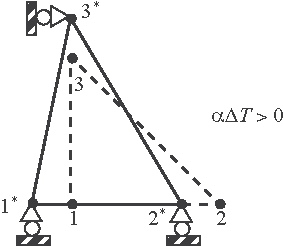
\includegraphics{Figure_16-7.pdf}
}{\caption{Initial configuration (dashed lines) and the displaced configuration (solid lines) of the self-strained truss in figure~\ref{fig16.6}.}\label{fig16.7}}

\begin{example*}[Five-bar truss]\label{ex16.4}The five-bar truss shown in figure~\ref{fig16.8} is restrained against rigid body motion, since joints 1 and 4 are fixed. pins All bars have the same extensional stiffness $E A$. Determine the restrained structural stiffness matrix $\left[K_{\alpha \alpha}\right]$.

\pagebreak

\processfigure[!h]{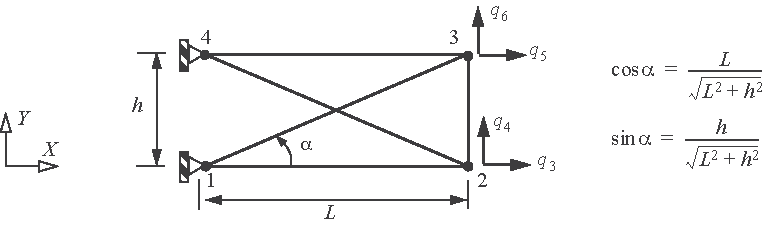
\includegraphics{Figure_16-8.pdf}
}{\caption{Five-bar truss.}\label{fig16.8}}

\vspace*{-1pc}

\subsubsection{Solution.} The dimensions of the restrained structural stiffness matrix is 4X4 in displacement degrees of freedom $q_{3}, q_{4}, q_{5}$, and $q_{6}$. The direction cosines for the truss bars are listed in table~\ref{tab16.3}.

\begin{table}[!h]%Table 16.3
\vspace*{-0.5pc}
\processtable{Direction cosines for the five-bar truss\label{tab16.3}}
{\begin{tabular}{@{}lcccccc@{}}\toprule
\colhead{Bar} & \colhead{$\theta$} & \colhead{$c$} & \colhead{$s$} & \colhead{$c^{2}$} & \colhead{$s^{2}$} & \colhead{${cs}$}\\\midrule
1-2 & $0^{\circ}$ & 1 & 0 & 1 & 0 & 0\\
1-3 & $\alpha$ & $\cos \alpha$ & $\sin \alpha$ & $\cos ^{2} \alpha$ & $\sin ^{2} \alpha$ & $\cos \alpha \sin \alpha$\\
2-3 & $90^{\circ}$  & 0 & 1 & 0 & 1 & 0\\
2-4 & $180^{\circ}-\alpha$ & $-\cos \alpha$ & $\sin \alpha$ & $\cos ^{2} \alpha$ & $\sin ^{2} \alpha$ & $-\cos \alpha \sin \alpha$\\
3-4 & $180^{\circ}$ & $-$1 & 0 & 1 & 0 & 0\\\botrule
\end{tabular}}{}
\vspace*{-1.5pc}
\end{table}

From eq.~(\ref{eq16.12}) the following member stiffness matrices are constructed using the direction cosines in table~\ref{tab16.3}. Only elements contributing to rows and columns 3, 4, 5, and 6 of the restrained structural stiffness matrix are extracted from the individual element stiffness matrices. These member stiffness matrices follow:
\begin{gather}\label{eq16.4a}\tag{a}
\left[K_{\alpha \alpha}\right]_{1-2}=\!\begin{array}{@{}c@{}}
\begin{array}{@{}ccc@{}}\phantom{0.}q_{3}& &q_{4}\phantom{0} \end{array}\\[6pt]\left[\begin{array}{@{}cr@{}}E A / L & 0 \\0 & 0\end{array}\right]\end{array}
\quad\left[K_{\alpha \alpha}\right]_{1-3}=\frac{E A}{L /(\cos \alpha)}\begin{array}{@{}c@{}}
{\arraycolsep=5pt\begin{array}{@{}cc@{}}q_{5}\phantom{0000} & \phantom{0000}q_{6} \end{array}}\\[6pt]\left[\begin{array}{@{}cc@{}}\cos ^{2} \alpha & \cos \alpha \sin \alpha \\\cos \alpha \sin \alpha & \sin ^{2} \alpha\end{array}\right]\end{array}=\frac{E A}{L}\begin{array}{@{}c@{}}{\arraycolsep=5pt\begin{array}{@{}cc@{}}
q_{5}\phantom{0000} & \phantom{0000}q_{6} \end{array}}\\[6pt]\left[\begin{array}{@{}ll@{}}\cos ^{3} \alpha & \cos ^{2} \alpha \sin \alpha \\\cos ^{2} \alpha \sin \alpha & \cos ^{2} \sin ^{2} \alpha\end{array}\right]\end{array}\\
\left[K_{\alpha \alpha}\right]_{2-3}=\left(\frac{E A}{L \tan \alpha}\right)\left[\begin{array}{@{}cccc@{}}0 & 0 & 0 & 0 \\0 & 1 & 0 & -1 \\0 & 0 & 0 & 0 \\0 & -1 & 0 & 1\end{array}\right]=\left(\frac{E A}{L}\right)\begin{array}{@{}c@{}}{\arraycolsep=7.5pt\begin{array}{@{}cccc@{}}q_{3}\phantom{.} & q_{4}\phantom{0} & q_{5}\phantom{0} & q_{6}\phantom{00} \end{array}}\\[6pt]\left[\begin{array}{@{}cccc@{}}0 & 0 & 0 & 0 \\0 & \cot \alpha & 0 & -\cot \alpha \\0 & 0 & 0 & 0 \\0 & -\cot \alpha & 0 & \cot \alpha\end{array}\right]\end{array}\quad \left[K_{\alpha \alpha}\right]_{3-4}=\begin{array}{@{}c@{}}\begin{array}{@{}cc@{}}\phantom{0}q_{5} & \phantom{00}q_{6} \end{array}\\[6pt]\left[\begin{array}{@{}cc@{}}E A / L & 0 \\0 & 0\end{array}\right]\end{array}.\label{eq16.4b}\tag{b}\\
\left[K_{\alpha \alpha}\right]_{2-4}=\left(\frac{E A}{L /(\cos \alpha)}\right)\left[\begin{array}{@{}cc@{}}\cos ^{2} \alpha & -\cos \alpha \sin \alpha \\-\cos \alpha \sin \alpha & \sin ^{2} \alpha\end{array}\right]=\frac{E A}{L}\begin{array}{@{}c@{}}\begin{array}{@{}cc@{}}q_{3}\phantom{0000} & \phantom{0000}q_{4} \end{array}\\[6pt]\left[\begin{array}{@{}cc@{}}\cos ^{3} \alpha & -\cos ^{2} \alpha \sin \alpha \\-\cos ^{2} \alpha \sin \alpha & \cos \alpha \sin ^{2} \alpha\end{array}\right]\end{array}.\label{eq16.4c}\tag{c}
\end{gather}
Assemblage of the restrained structural stiffness matrix is accomplished by adding like row and column elements from the stiffness matrices of each truss bar. The result for the restrained structural stiffness matrix is\pagebreak
\begin{align}\label{eq16.4d}\tag{d}
\left[K_{\alpha \alpha}\right]=\left(\frac{E A}{L}\right)\begin{array}{@{}c@{}}{\begin{array}{@{\hspace*{-6pt}}c@{\qquad\qquad\qquad}c@{\qquad\qquad\qquad}c@{\qquad\qquad\qquad\;\;}c@{}}
\hspace*{-0.8pc}q_{3}\hspace*{6pt} &\hspace*{6pt} q_{4}&\hspace*{9pt} \!\!q_{5}\hspace*{-6pt} & \phantom{00}q_{6} \end{array}}\\[6pt]\left[\begin{array}{@{}cccc@{}}\left(1+\cos ^{3} \alpha\right) & -\cos ^{2} \alpha \sin \alpha & 0 & 0 \\-\cos ^{2} \alpha \sin \alpha & \left(\cot \alpha+\cos \alpha \sin ^{2} \alpha\right) & 0 & -\cot \alpha \\0 & 0 & \left(\cos ^{3} \alpha+1\right) & \cos ^{2} \alpha \sin \alpha \\0 & -\cot \alpha & \cos ^{2} \alpha \sin \alpha & \left(\cos \alpha \sin ^{2} \alpha+\cot \alpha\right)\end{array}\right]\end{array}.
\end{align}
Note that the matrix is symmetric and the sum of the column elements do not add to zero. If we take $\alpha=30^{\circ}$, then the restrained structural stiffness matrix reduces to
\begin{align}\label{eq16.4e}\tag{e}
\left[K_{\alpha \alpha}\right]=\left(\frac{E A}{L}\right)\begin{array}{@{}c@{}}\begin{array}{@{}c@{\qquad\qquad}c@{\qquad\qquad\quad}c@{\qquad\qquad}c@{}}q_{3} & q_{4} & q_{5} & q_{6} \end{array}\\[3pt]\left[\begin{array}{@{}cccc@{}}1+(3 \sqrt{3}) / 8 & -3 / 8 & 0 & 0 \\-3 / 8 & \sqrt{3}(9 / 8) & 0 & -\sqrt{3} \\0 & 0 & 1+(3 \sqrt{3}) / 8 & 3 / 8 \\0 & -\sqrt{3} & 3 / 8 & \sqrt{3}(9 / 8)\end{array}\right]\end{array}. \\[-1.4pc] \nonumber {\hfill\qed\hspace*{-7.4pc}}
\end{align}
\end{example*}

\vspace*{-1.6pc}

\begin{example}[Using symmetry to reduce problem size]\label{ex16.5}Consider the five-bar truss problem of example~\ref{ex16.4} with $\alpha=30^{\circ}$ that is subject to prescribed nodal forces $Q_{3}, Q_{4}, Q_{5}, \text { and } Q_{6}$. Use symmetry to reduce the problem size to solve for the unknown joint displacements.

\processfigure[!h]{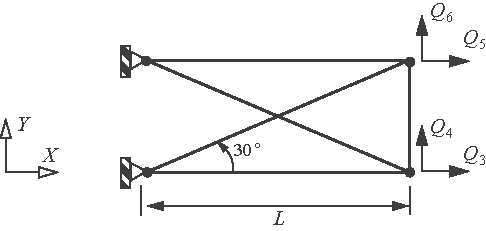
\includegraphics{Figure_16-9.pdf}
}{\caption{Five-bar truss of example~\ref{ex16.5}.}\label{fig16.9}}

\subsubsection{Solution.} We note that the structure and boundary conditions are symmetric about a horizontal axis through the center of the truss. The joint displacements and corresponding forces can be decomposed into a symmetric and antisymmetric sets about this horizontal axis of symmetry as shown in figure~\ref{fig16.10}. The joint displacements and the corresponding forces are related to the symmetric and antisymmetric counterparts by
\begin{align}\label{eq16.5a}\tag{a}
\left[\begin{array}{@{}l@{}}q_{3} \\q_{4} \\q_{5} \\q_{6}\end{array}\right]=\left[\begin{array}{@{}c@{}}x_{a} \\-y_{a} \\x_{a} \\y_{a}\end{array}\right]+\left[\begin{array}{@{}c@{}}-x_{b} \\y_{b} \\x_{b} \\y_{b}\end{array}\right]=\left[\begin{array}{@{}cccc@{}}1 & 0 & -1 & 0 \\0 & -1 & 0 & 1 \\1 & 0 & 1 & 0 \\0 & 1 & 0 & 1\end{array}\right]\left[\begin{array}{@{}l@{}}x_{a} \\y_{a} \\x_{b} \\y_{b}\end{array}\right]\mbox{, and }\left[\begin{array}{@{}c@{}}Q_{3} \\Q_{4} \\Q_{5} \\Q_{6}\end{array}\right]=\left[\begin{array}{@{}c@{}}X_{a} \\-Y_{a} \\X_{a} \\Y_{a}\end{array}\right]+\left[\begin{array}{@{}c@{}}-X_{b} \\Y_{b} \\X_{b} \\Y_{b}\end{array}\right]=\left[\begin{array}{@{}cccc@{}}1 & 0 & -1 & 0 \\0 & -1 & 0 & 1 \\1 & 0 & 1 & 0 \\0 & 1 & 0 & 1\end{array}\right]\left[\begin{array}{@{}c@{}}X_{a} \\Y_{a} \\X_{b} \\Y_{b}\end{array}\right].
\end{align}

\processfigure[!h]{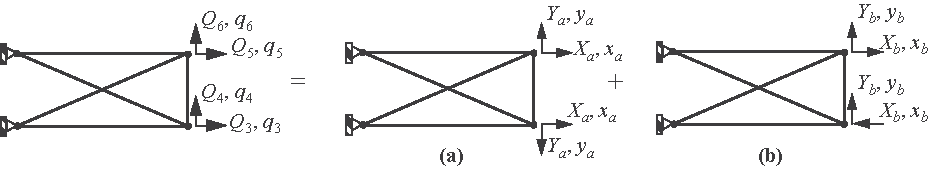
\includegraphics{Figure_16-10.pdf}
}{\caption{(a) Symmetric truss. (b) Antisymmetric truss.}\label{fig16.10}}

\vspace*{-1pc}

\noindent The expressions in eq. (\textbf{\ref{eq16.5a}}) are written in compact form as
\begin{align}\label{eq16.5b}\tag{b}
\left\{q_{\alpha}\right\}=[A]\{x\}\mbox{, and }\left\{Q_{\alpha}\right\}=[A]\{X\},
\end{align}

\vspace*{-1pc}\pagebreak

\noindent where the elements of the 4X4 matrix $[A]$ are either –1, 0, or 1.The force vector is related to the displacement vector by $\left\{Q_{\alpha}\right\}=\left[K_{\alpha \alpha}\right]\left\{q_{\alpha}\right\}$, where matrix $\left[K_{\alpha \alpha}\right]$ is given by eq. (\textbf{\ref{eq16.5e}}) in example~\ref{ex16.4}. Substitute eq. (\textbf{\ref{eq16.5b}}) into the matrix equation relating the force vector to the displacement vector to get
\begin{align}\label{eq16.5c}\tag{c}
[A]\{X\}=\left[K_{\alpha \alpha}\right][A]\{x\}.
\end{align}
Pre-multiply eq. (\textbf{\ref{eq16.5c}}) by the inverse of matrix $[A]$ to find
\begin{align}\label{eq16.5d}\tag{d}
\{X\}=[A]^{-1}\left[K_{\alpha \alpha}\right][A]\{x\}.
\end{align}
Define stiffness matrix by $\left[\bar{K}_{\alpha \alpha}\right]=[A]^{-1}\left[K_{\alpha \alpha}\right][A]$. The the matrices to compute $\left[\bar{K}_{\alpha \alpha}\right]$ are
\begin{align}\label{eq16.5e}\tag{e}
\left[\bar{K}_{\alpha \alpha}\right]=\frac{1}{2}\left[\begin{array}{@{}cccc@{}}1 & 0 & 1 & 0 \\0 & -1 & 0 & 1 \\-1 & 0 & 1 & 0 \\0 & 1 & 0 & 1\end{array}\right]\left(\frac{E A}{L}\right)\left[\begin{array}{ccccc}1+(3 \sqrt{3}) / 8 & -3 / 8 & 0 & 0  \\-3 / 8 & \sqrt{3}(9 / 8) & 0 & -\sqrt{3} \\0 & 0 & 1+(3 \sqrt{3}) / 8 & 3 / 8\\0 & -\sqrt{3} &3 / 8 & \sqrt{3}(9 / 8)  \end{array}\right]
\left[\begin{array}{@{}cccc@{}}1 & 0 & -1 & 0 \\0 & -1 & 0 & 1 \\1 & 0 & 1 & 0 \\0 & 1 & 0 & 1\end{array}\right].
\end{align}
The result of the matrix multiplications in eq. (\textbf{\ref{eq16.5e}}) is
\begin{align}\label{eq16.5f}\tag{f}
\left[\bar{K}_{\alpha \alpha}\right]=\frac{E A}{L}\left|\begin{array}{@{}cccc@{}}1+(3 \sqrt{3}) / 8 & 3 / 8 & 0 & 0 \\3 / 8 & (17 \sqrt{3}) / 8 & 0 & 0 \\0 & 0 & 1+(3 \sqrt{3}) / 8 & 3 / 8 \\0 & 0 & 3 / 8 & (\sqrt{3}) / 8\end{array}\right|=\left[\begin{array}{@{}c@{}}{\left[\bar{K}_{a}\right]\left[\begin{array}{@{}c@{}}0_{2 X 2}\end{array}\right]} \\[6pt]\left.\left[0_{2 X 2}\right]\left[\bar{K}_{b}\right]\right]\end{array}\right].
\end{align}
Note that the partitioned form of $\left[\bar{K}_{\alpha \alpha}\right]$ is diagonal, and the 2X2 sub-matrices on the diagonal are
\begin{align}\label{eq16.5g}\tag{g}
\left[\bar{K}_{a}\right]=\frac{E A}{L}\left[\begin{array}{@{}cc@{}}1+\frac{3 \sqrt{3}}{8} & \frac{3}{8} \\[6pt]\frac{3}{8} & \frac{17 \sqrt{3}}{8}\end{array}\right]\mbox{, and }\left[\bar{K}_{b}\right]=\frac{E A}{L}\left[\begin{array}{@{}cc@{}}1+\frac{3 \sqrt{3}}{8} & \frac{3}{8} \\[6pt]\frac{3}{8} & \frac{\sqrt{3}}{8}\end{array}\right].
\end{align}
The inverses of the matrices in eq. (\textbf{\ref{eq16.5g}}) are
\begin{align}\label{eq16.5h}\tag{h}
\left[\bar{K}_{a}\right]^{-1}=\frac{L}{E A} \left[\begin{array}{@{}l@{}}\frac{17}{181}(17-6 \sqrt{3}) \frac{1}{181}(18-17 \sqrt{3}) \\[6pt]\frac{1}{181}(18-17 \sqrt{3}) \frac{1}{543}(9+82 \sqrt{3})\end{array}\right]\mbox{, and }\left[\bar{K}_{b}\right]^{-1}=\frac{L}{E A}\left[\begin{array}{@{}cc@{}}1 & -\sqrt{3} \\-\sqrt{3} & (3+8 / \sqrt{3})\end{array}\right].
\end{align}
Then the inverse of eq. (\textbf{\ref{eq16.5f}}) is given by
\begin{align}\label{eq16.5i}\tag{i}
\left[\bar{K}_{\alpha \alpha}\right]^{-1}=\left[\begin{array}{@{}l@{}}{\left[\bar{K}_{a}\right]^{-1}\left[\begin{array}{@{}l@{}}0_{2 X 2}\end{array}\right]} \\[6pt]{\left[0_{2 X 2}\right]\left[\bar{K}_{b}\right]^{-1}}\end{array}\right].
\end{align}
Hence, the solution for the displacement vector $\{x\}$ in terms of the force vector $\{X\}$ is
\begin{align}\label{eq16.5j}\tag{j}
\{x\}=\left[\bar{K}_{\alpha \alpha}\right]^{-1}\{X\}.
\end{align}
From eq. (\textbf{\ref{eq16.5b}}) $\{x\}=[A]^{-1}\left\{q_{\alpha}\right\}\mbox{ and }\{X\}=[A]^{-1}\left\{Q_{\alpha}\right\}$ Substitute the latter relations into eq. (\textbf{\ref{eq16.5j}}) to get
\begin{align}\label{eq16.5k}\tag{k}
[A]^{-1}\left\{q_{\alpha}\right\}=\left[\bar{K}_{\alpha \alpha}\right]^{-1}[A]^{-1}\left\{Q_{\alpha}\right\}.
\end{align}
Pre-multiply eq. (\textbf{\ref{eq16.5k}}) by matrix $[A]$ to write the result for the unknown displacements as
\begin{align}\label{eq16.5l}\tag{l}
\left\{q_{\alpha}\right\}=\left[C_{\alpha \alpha}\right]\left\{Q_{\alpha}\right\},
\end{align}
where the compliance matrix is
\begin{align}\label{eq16.5m}\tag{m}
\left[C_{\alpha \alpha}\right]=[A]\left[\bar{K}_{\alpha \alpha}\right]^{-1}[A]^{-1}=\frac{L}{E A}\left[\begin{array}{@{}cccc@{}}0.810306 & 0.897641 & -0.189694 & 0.83441 \\0.897641 & 3.94847 & -0.83441 & 3.67033 \\-0.189694 & -0.83441 & 0.810306 & -0.897641 \\0.83441 & 3.67033 & -0.897641 & 3.94847\end{array}\right].
\end{align}
The compliance matrix in eq. (\textbf{\ref{eq16.5m}}) was obtained by inverting two 2X2 sub-matrices, rather than directly inverting the 4X4 stiffness matrix $\left[K_{\alpha \alpha}\right]$. Exploiting the symmetry conditions as illustrated in figure~\ref{fig16.10}, reduces the number of computations to find the inverse of matrix $\left[K_{\alpha \alpha}\right]$.
\end{example}

\vspace*{-1pc}

\section{Structures containing beam members}\label{sec16.2}

Consider a prismatic, homogeneous beam that is referenced to the Cartesian system \textit{x-y-z}. The $z$-coordinate is the longitudinal axis, and the coordinates $x$ and $y$ define cross-sectional axes with the origin at the centroid. Assume at least one axis $x$ and/or $y$ is an axis of symmetry so that the product area moment $I_{x y}=0$. External loads are specified as a transverse distributed load $f_{y}(z)$ as shown in figure~\ref{fig3.8} on page \pageref{fig3.8}, and we assume a change in temperature in the form $\Delta T(y, z)=\tau_{y}(z) y(s)$. For this form of the prescribed change in temperature the thermal axial force $N_{T}=0$ in eq.~(\ref{eq3.75}), and thermal bending moment $M_{x T} \neq 0$ in eq.~(\ref{eq3.78}). The plane of loading $f_{y}(z)$ coincides with the locus of shear centers. Hence, the beam bends in the \textit{y-z} plane. Assume the \textbf{Euler-Bernoulli} theory in which the transverse shears in eq.~(\ref{eq4.28}) on page \pageref{eq4.28} equal zero. That is,
\begin{align}\label{eq16.19}
\psi_{y}=\frac{d v}{d z}+\phi_{x}=0.
\end{align}
(Refer to the discussion about the Euler-Bernoulli theory preceding table~\ref{tab4.4} on page \pageref{tab4.4}.) Equilibrium differential equations (\ref{eq3.54}) and (\ref{eq3.55}) are
\begin{align}\label{eq16.20}
\frac{d V_{y}}{d z}+f_{y}=0 \quad \frac{d M_{x}}{d z}-V_{y}=0.
\end{align}
Hooke's law (\ref{eq3.79}) on page \pageref{eq3.79} for bending is
\begin{align}\label{eq16.21}
M_{x}+M_{x T}=E I_{x x} \frac{d \phi_{x}}{d z},
\end{align}
where the thermal bending moment is given by eq.~(\ref{eq3.78}) on page \pageref{eq3.78}. The change in temperature on the contour is $\Delta T=\tau_{y}(z) y(s)$ and eq.~(\ref{eq3.78}) simplifies to
\begin{align}\label{eq16.22}
M_{x T}=E I_{x x} \alpha \tau_{y}(z).
\end{align}
Combine eqs. (\ref{eq16.20}), (\ref{eq16.21}), and (\ref{eq16.22}) to get the governing differential equation for the deflection of the beam~as
\begin{align}\label{eq16.23}
E I_{x x} \frac{d^{4} v}{d z^{4}}=f_{y}(z)-E I_{x x} \alpha \frac{d^{2} \tau_{y}}{d z^{2}} \quad 0<z<L.
\end{align}
Let $q_{1}$ denote the $y$-direction displacement of the neutral axis at $z = 0$, $q_{2}$ the rotation of the cross section about the $x$-axis at $z = 0$, $q_{3}$ the $y$-direction displacement of the neutral axis at $z = \textit{L}$, and $q_{4}$ the rotation of the cross section about the $x$-axis at $z = \textit{L}$. Then the boundary conditions at the ends of the beam are
\begin{align}\label{eq16.24}
v(0)=q_{1} \quad \phi_{x}(0)=q_{2} \quad v(L)=q_{3} \quad \phi_{x}(L)=q_{4}.
\end{align}
The governing boundary value problem defined by (\ref{eq16.23}) and (\ref{eq16.24}) is depicted in figure~\ref{fig16.11}(a). Actions corresponding to the generalized displacements $q_1$, $q_2$, $q_3$, and $q_4$ are denoted by $\textit{Q}_1$, $\textit{Q}_2$, $\textit{Q}_3$, and $\textit{Q}_4$, respectively. Free body diagrams at the beginning joint ($z = 0$) and the end joint ($z = \textit{L}$) are shown in figure~\ref{fig16.11}(b). Equilibrium at the joints leads to
\begin{align}\label{eq16.25}
Q_{1}+V_{y}(0)=0 \quad Q_{2}+M_{x}(0)=0 \quad Q_{3}-V_{y}(L)=0 \quad Q_{4}-M_{x}(L)=0.
\end{align}

\processfigure[!h]{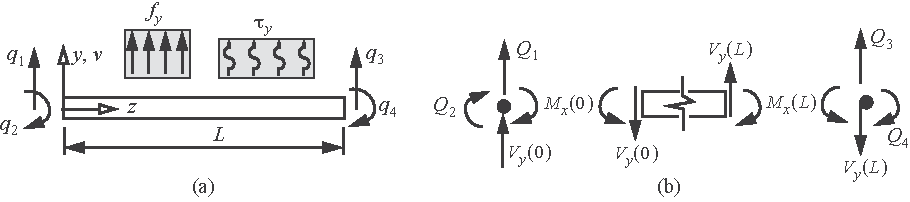
\includegraphics{Figure_16-11.pdf}
}{\caption{(a) The boundary value problem for the beam. (b) Joint equilibrium.}\label{fig16.11}}

The solution to the governing boundary value problem is sought by the method of superposition. Let the lateral displacement be represented by the sum of displacements in the form
\begin{align}\label{eq16.26}
v(z)=v_{0}(z)+v_{1}(z).
\end{align}
The boundary value problem for $v_{0}(z)$ is selected as
\begin{gather}\label{eq16.27}
\begin{split}E I v_{0}{ }^{\prime \prime \prime \prime}=f_{y}(z)-E I \alpha \tau_{y}^{\prime \prime} \quad 0<z<L\hspace*{2pc} \\
v_{0}(0)=0 \quad-v_{0}^{\prime}(0)=0 \quad v_{0}(L)=0 \quad-v_{0}^{\prime}(L)=0
\end{split}.
\end{gather}
As a consequence the boundary value problem for $v_{1}(z)$ is
\begin{align}\label{eq16.28}
\begin{array}{@{}ccc@{}}E I v_{1}^{\prime \prime \prime\prime}=0 & 0<z<L \\v_{1}(0)=q_{1} \quad-v_{0}^{\prime}(0)=q_{2} & v_{0}(L)=q_{3} \quad-v_{0}^{\prime}(L)=q_{4}\end{array}.
\end{align}
In eqs. (\ref{eq16.27}) and (\ref{eq16.28}) ordinary derivatives with respect to $z$ are denoted by primes $\big($e.g., $v^{\prime}=\frac{d v}{d z}\big)$. Also, we let $E I_{x x}=E I$. The boundary value problem (\ref{eq16.27}) for displacement function $v_{0}(z)$ consists of an inhomogeneous differential equation with homogeneous boundary conditions, while the boundary value problem (\ref{eq16.28}) for displacement function $v_{1}(z)$ consists of a homogeneous differential equation with inhomogeneous boundary conditions. Since the displacements and rotations vanish at the end points of the beam in the boundary value problem for $v_{0}(z)$, the solution for it will lead to \textbf{fixed-end actions} in the matrix structural analysis method. That is, the fixed-end action problem accounts for distributed load intensity $f_{y}(z)$, and the distributed temperature gradient $\tau_{y}(z)$. By superposition the total bending moment is
\begin{align}\label{eq16.29}
M_{x}(z)=-E I\left(v_{0}^{\prime \prime}+v_{1}^{\prime \prime}\right)-E I \alpha \tau_{y}=M_{x}^{0}+M_{x}^{1},
\end{align}
where the bending moments from the separate boundary value problems are
\begin{align}\label{eq16.30}
M_{x}^{0}=-E I v_{0}^{\prime \prime}-E I \alpha \tau_{y} \quad M_{x}^{1}=-E I v_{1}^{\prime \prime}.
\end{align}
The shear force is the sum
\begin{align}\label{eq16.31}
V_{y}(z)=V_{y}^{0}+V_{y}^{1},
\end{align}
where the shear forces from the separate boundary value problems are
\begin{align}\label{eq16.32}
V_{y}^{0}=\frac{d}{d z}\left(M_{x}^{0}\right) \quad V_{y}^{1}=\frac{d}{d z}\left(M_{x}^{1}\right).
\end{align}

\subsection{ Boundary value problem (\ref{eq16.28}). Generalized displacements at the boundaries}\label{sec16.2.1}

The general solution for $v_{1}(z)$ satisfying the differential equation in boundary value problem (\ref{eq16.28}) is a cubic polynomial in the longitudinal coordinate, which is written as
\begin{align}\label{eq16.33}
v_{1}(z)=c_{3} \frac{z^{3}}{6}+c_{2} \frac{z^{2}}{2}+c_{1} z+c_{0},
\end{align}
where the constants $c_{3}, c_{2}, c_{1}$, and $c_{0}$ are to be determined by the four boundary conditions specified in eq.~(\ref{eq16.28}). Substitute the general solution (\ref{eq16.33}) into these four boundary conditions and write result as
\begin{align}\label{eq16.34}
\left[\begin{array}{@{}cccc@{}}0 & 0 & 0 & 1 \\0 & 0 & -1 & 0 \\ L^{3} / 6 & L^{2} / 2 & L & 1 \\ -L^{2} / 2 & -L & -1 & 0\end{array}\right]\left[\begin{array}{@{}l@{}}c_{3} \\ c_{2} \\ c_{1} \\ c_{0}\end{array}\right]=\left[\begin{array}{@{}l@{}}q_{1} \\ q_{2} \\ q_{3} \\q_{4}\end{array}\right].
\end{align}
Solve eq.~(\ref{eq16.34}) for the constants $c_{3}, c_{2}, c_{1}$, and $c_{0}$ to get
\begin{align}\label{eq16.35}
\left[\begin{array}{@{}l@{}}c_{3} \\c_{2} \\c_{1} \\c_{0}\end{array}\right]=\left[\begin{array}{@{}cccc@{}}12 / L^{3} & -6 / L^{2} & -12 / L^{3} & -6 / L^{2} \\-6 / L^{2} & 4 / L & 6 / L^{2} & 2 / L \\0 & -1 & 0 & 0 \\1 & 0 & 0 & 0\end{array}\right]\left[\begin{array}{@{}l@{}}q_{1} \\q_{2} \\q_{3} \\q_{4}\end{array}\right].
\end{align}
Substituting eq.~(\ref{eq16.35}) for the constants $c_{3}, c_{2}, c_{1}$, and $c_{0}$ into eq.~(\ref{eq16.33}) leads to
\begin{align}\label{eq16.36}
v_{1}(z)=\frac{1}{6}\left(\frac{12}{L^{3}} q_{1}-\frac{6}{L^{2}} q_{2}-\frac{12}{L^{3}} q_{3}-\frac{6}{L^{2}} q_{4}\right) z^{3}+\frac{1}{2}\left(-\frac{6}{L^{2}} q_{1}+\frac{4}{L} q_{2}+\frac{6}{L^{2}} q_{3}+\frac{2}{L} q_{4}\right) z^{2}+\left(-q_{2}\right) z+q_{1}.
\end{align}
Rearrange eq.~(\ref{eq16.36}) to the form
\begin{align}\label{eq16.37}
v_{1}(z)=\left(2 \frac{z^{3}}{L^{3}}-3 \frac{z^{2}}{L^{2}}+1\right) q_{1}+\left(-\frac{z^{3}}{L^{2}}+2 \frac{z^{2}}{L}-z\right) q_{2}+\left(-2 \frac{z^{3}}{L^{3}}+3 \frac{z^{2}}{L^{2}}\right) q_{3}+\left(-\frac{z^{3}}{L^{2}}+\frac{z^{2}}{L}\right) q_{4}.
\end{align}
Equation (\ref{eq16.37}) is further written in the matrix form
\begin{align}\label{eq16.38}
v_{1}(z)=\left[\eta_{1}(z)\ \eta_{2}(z)\ \eta_{3}(z)\ \eta_{4}(z)\right]\left[\begin{array}{@{}l@{}}q_{1} \\q_{2} \\q_{3} \\q_{4}\end{array}\right]=[\eta(z)]\{q\}.
\end{align}
The \textit{shape functions}, or \textit{interpolation functions}, are defined as
\begin{align}\label{eq16.39}
\eta_{1}(z) \equiv 2 \frac{z^{3}}{L^{3}}-3 \frac{z^{2}}{L^{2}}+1 \quad \eta_{2}(z) \equiv-\frac{z^{3}}{L^{2}}+2 \frac{z^{2}}{L}-z \quad \eta_{3}(z) \equiv-2 \frac{z^{3}}{L^{3}}+3 \frac{z^{2}}{L^{2}} \quad \eta_{4}(z) \equiv-\frac{z^{3}}{L^{2}}+\frac{z^{2}}{L}.
\end{align}
From eq.~(\ref{eq16.19}) the rotation associated with the lateral displacement function $v_{1}(z)$ is given by
\begin{align}\label{eq16.40}
\phi_{x}(z)=-v_{1}^{\prime}(z)=\left[-\eta_{1}^{\prime}(z)-\eta_{2}^{\prime}(z)-\eta_{3}^{\prime}(z)-\eta_{4}{ }^{\prime}(z)\right]\left[\begin{array}{@{}l@{}}q_{1} \\q_{2} \\q_{3} \\q_{4}\end{array}\right],
\end{align}
where
\begin{align}\label{eq16.41}
\eta_{1}^{\prime}(z)=\frac{6}{L^{3}} z^{2}-6 \frac{z}{L^{2}} \quad \eta_{2}^{\prime}(z)=-3 \frac{z^{2}}{L^{2}}+4 \frac{z}{L}-1 \quad \eta_{3}{ }^{\prime}(z)=-6 \frac{z^{2}}{L^{3}}+6 \frac{z}{L^{2}} \quad \eta_{4}^{\prime}(z)=-3 \frac{z^{2}}{L^{2}}+2 \frac{z}{L}.
\end{align}
These interpolation functions have the following properties at the end points, or joints, of the beam member:
\begin{align}\label{eq16.42}
\begin{array}{@{}llll@{}}\eta_{1}(0)=1 & \eta_{2}(0)=0 & \eta_{3}(0)=0 & \eta_{4}(0)=0 \\\eta_{1}^{\prime}(0)=0 & \eta_{2}^{\prime}(0)=-1 & \eta_{3}^{\prime}(0)=0 & \eta_{4}^{\prime}(0)=0 \\\eta_{1}(L)=0 & \eta_{2}(L)=0 & \eta_{3}(L)=1 & \eta_{4}(L)=0 \\\eta_{1}^{\prime}(L)=0 & \eta_{2}^{\prime}(L)=0 & \eta_{3}^{\prime}(L)=0 & \eta_{4}^{\prime}(L)=-1\end{array}.
\end{align}

The distributions of the shear force (\ref{eq16.32}) and the bending moment (\ref{eq16.30}) for the boundary value problem (\ref{eq16.28}) are
\begin{align}\label{eq16.43}
\left[\begin{array}{@{}l@{}}V_{y}^{1}(z) \\[6pt] M_{x}^{1}(z)\end{array}\right]=E I\left[\begin{array}{@{}c@{}}-v_{1}^{\prime \prime \prime} \\[6pt]-v_{1}^{\prime \prime}\end{array}\right]=E I\left[\begin{array}{@{}cccc@{}}-\eta_{1}{ }^{\prime \prime \prime} & -\eta_{2}^{\prime \prime \prime} & -\eta_{3}^{\prime \prime \prime} & -\eta_{4}^{\prime \prime \prime} \\-\eta_{1}{ }^{\prime \prime} & -\eta_{2}^{\prime \prime} & -\eta_{3}^{\prime \prime} & -\eta_{4}^{\prime \prime}\end{array}\right]\left[\begin{array}{@{}l@{}}q_{1} \\q_{2} \\q_{3} \\q_{4}\end{array}\right].
\end{align}
Substitute for the shape functions from eq.~(\ref{eq16.39}) into eq.~(\ref{eq16.43}) to find
\begin{align}\label{eq16.44}
\left[\begin{array}{@{}c@{}}V_{y}^{1}(z) \\[6pt] M_{x}^{1}(z)\end{array}\right]=E I\left[\begin{array}{c:c:c:c}-\frac{12}{L^{3}} & \frac{6}{L^{2}} & \frac{12}{L^{3}} & \frac{6}{L^{2}} \\[12pt]\frac{6}{L^{2}}-\frac{12 z}{L^{3}} & -\frac{4}{L}+\frac{6 z}{L^{2}} & -\frac{6}{L^{2}}+\frac{12 z}{L^{3}} & -\frac{2}{L}+\frac{6 z}{L^{2}}\end{array}\right]\left[\begin{array}{@{}l@{}}q_{1} \\q_{2} \\q_{3} \\q_{4}\end{array}\right].
\end{align}
Since eq.~(\ref{eq16.44}) relates the internal actions consisting of the shear force and the bending moment to the joint displacement vector, it defines the 2X4 \textit{stress matrix }as
\begin{align}\label{eq16.45}
\left[S^{1}(z)\right] \equiv E I\left[\begin{array}{c:c:cc}-\frac{12}{L^{3}} & \frac{6}{L^{2}} & \frac{12}{L^{3}} & \frac{6}{L^{2}} \\[12pt]\frac{6}{L^{2}}-\frac{12 z}{L^{3}} & -\frac{4}{L}+\frac{6 z}{L^{2}} & -\frac{6}{L^{2}}+\frac{12 z}{L^{3}} & -\frac{2}{L}+\frac{6 z}{L^{2}}\end{array}\right],
\end{align}
such that
\begin{align}\label{eq16.46}
\left[\begin{array}{@{}c@{}}V_{y}^{1}(z) \\[6pt]M_{x}^{1}(z)\end{array}\right]=\left[S^{1}(z)\right]\left[\begin{array}{@{}l@{}}q_{1} \\q_{2} \\q_{3} \\q_{4}\end{array}\right] \quad 0 \leq z \leq L.
\end{align}
Equilibrium at the joints $z = 0$ and $z = \textit{L}$ in (\ref{eq16.25}) leads to
\begin{align}\label{eq16.47}
\left[\begin{array}{@{}l@{}}Q_{1}^{1} \\[6pt]Q_{2}^{1}\end{array}\right]=\left[\begin{array}{@{}c@{}}-V_{y}^{1}(0) \\[6pt] -M_{x}^{1}(0)\end{array}\right]=\left[-S^{1}(0)\right]\left[\begin{array}{@{}l@{}}q_{1} \\q_{2} \\q_{3} \\q_{4}\end{array}\right]\left[\begin{array}{@{}l@{}}Q_{3}^{1} \\[6pt]Q_{4}^{1}\end{array}\right]=\left[\begin{array}{@{}c@{}}V_{y}^{1}(L) \\[6pt] M_{x}^{1}(L)\end{array}\right]=\left[S^{1}(L)\right]\left[\begin{array}{@{}l@{}}q_{1} \\q_{2} \\q_{3} \\q_{4}\end{array}\right].
\end{align}
Combine these results into one matrix equation to get
\begin{align}\label{eq16.48}
\left[\begin{array}{@{}c@{}}Q_{1}^{1} \\[6pt] Q_{2}^{1} \\[6pt] Q_{3}^{1} \\[6pt] Q_{4}^{1}\end{array}\right]=\left[\begin{array}{@{}c@{}}\left[-S^{1}(0)\right] \\{\left[S^{1}(L)\right]}\end{array}\right]\left[\begin{array}{@{}l@{}}q_{1} \\q_{2} \\q_{3} \\q_{4}\end{array}\right] \quad \text { or } \quad\begin{array}{@{}c@{}}\left\{Q^{1}\right\}\\4X1\end{array}=\begin{array}{@{}c@{}}[K]\\4X4\end{array} \begin{array}{@{}c@{}}\{q\}\\ 4X1\end{array}.
\end{align}
The beam element stiffness matrix is defined by
\begin{align}\label{eq16.49}
[K]=\left[\begin{array}{@{}c@{}}{\left[-S^{1}(0)\right]} \\[6pt]\left.\left[S^{1}(L)\right]\right]\end{array}\right], \quad \text{which evaluates to } \boxed{[K]=E I\left[\begin{array}{@{}cccc@{}}\frac{12}{L^{3}} & \frac{-6}{L^{2}} & \frac{-12}{L^{3}} & \frac{-6}{L^{2}} \\[6pt]\frac{-6}{L^{2}} & \frac{4}{L} & \frac{6}{L^{2}} & \frac{2}{L} \\[6pt]\frac{-12}{L^{3}} & \frac{6}{L^{2}} & \frac{12}{L^{3}} & \frac{6}{L^{2}} \\[6pt]\frac{-6}{L^{2}} & \frac{2}{L} & \frac{6}{L^{2}} & \frac{4}{L}\end{array}\right]}.
\end{align}
The stiffness matrix of the beam member (\ref{eq16.49}) has the following properties:
\begin{itemize}
\item It is symmetric, because the material is linear elastic and the displacements and rotations of the beam are assumed small.

\item The column elements satisfy equilibrium for each unit displacement state.

For example consider unit displacement state one with $\{q\}=\left[\begin{array}{@{}l@{\;}l@{\;}l@{\;}l@{}}1 & 0 & 0 & 0\end{array}\right]^{T}$.

The corresponding generalized joint forces are
\[
\left\{Q^{1}\right\}=\left[\begin{array}{@{}llll@{}}
Q_{1}^{1} & Q_{2}^{1} & Q_{3}^{1} & Q_{4}^{1}\end{array}\right]^{T}=E I\left[\frac{12}{L^{3}} \frac{-6}{L^{2}} \frac{-12}{L^{3}} \frac{-6}{L^{2}}\right]^{T}(1).
\]

The sum of the vertical forces is $Q_{1}^{1}+Q_{3}^{1}=E I\left[\frac{12}{L^{3}}+\left(\frac{-12}{L^{3}}\right)\right](1)=0$.

The sum of moments about the center of the beam clockwise positive are:
\[
\frac{L}{2} Q_{1}^{1}+Q_{2}^{1}-\frac{L}{2} Q_{3}^{1}+Q_{4}^{1}=E I\left[\frac{L}{2}\left(\frac{12}{L^{3}}\right)+\left(\frac{-6}{L^{2}}\right)-\frac{L}{2}\left(\frac{-12}{L^{3}}\right)+\frac{-6}{L^{2}}\right](1)=0.
\]

As result of the four unit displacement states the elements of the beam stiffness matrix satisfy the following relationships.

The sum of rows one and three equals zero. $\sum\limits_{j=1}^4 k_{1 j}+k_{3 j}=0$.

The sum of \textit{L/2} times row one plus row two minus \textit{L/2} times row three plus row four is equal to zero. $\sum\limits_{j=1}^4(L / 2) k_{1 j}+k_{2 j}-(L / 2) k_{3 j}+k_{4 j}=0$.

Since the stiffness matrix is symmetric, the column elements satisfy the same relationships as do the row elements

\item ${Det}[K]=0$, since the beam member is not restrained against rigid body displacement.

\item Its diagonal elements are positive.
\end{itemize}

\subsection{ Boundary value problem (\ref{eq16.27}). Fixed-end actions}\label{sec16.2.2}

The fixed-end action vector is computed from the boundary value problem (\ref{eq16.27}) to account for the distributed load and the temperature distribution in the direct stiffness method. Many practical problems can be analyzed with a linear distribution of the load intensity and a linear distribution of the cross-sectional temperature gradient. These linear distributions are specified as
\begin{align}\label{eq16.50}
f_{y}(z)=f_{y 1}(1-z / L)+f_{f y 2}(z / L)\mbox{ and }\tau_{y}(z)=\tau_{y 1}(1-z / L)+\tau_{y 2}(z / L).
\end{align}
The values of the distributed load and temperature gradient at $z = 0$ are $f_{y 1}$ and $\tau_{y 1}$, respectively. At $z = \textit{L}$, the distributed load intensity is $f_{y 2}$ and the temperature gradient is $\tau_{y 2}$. The boundary value problem (\ref{eq16.27}) reduces~to
\begin{align}\label{eq16.51}
\begin{array}{clc}E I v_{0}{}^{\prime \prime \prime\prime} & =f_{y 1}(1-z / L)+f_{f y 2}(z / L) & 0<z<L \\v_{0}(0)=0 & -v_{0}^{\prime}(0)=0 \quad v_{0}(L)=0 & -v_{0}^{\prime}(L)=0\end{array}.
\end{align}
The solution for displacement $v_{0}(z)$ is
\begin{align}\label{eq16.52}
v_{0}(z)=\left[\frac{(L-z)^{2}(3 L-z) z^{2}}{120 E I L}\right] f_{y 1}+\left[\frac{(L-z)^{2}(2 L+z) z^{2}}{120 E I L}\right] f_{y 2}.
\end{align}
The distribution of the transverse shear force (\ref{eq16.32}) and the bending moment (\ref{eq16.30}) are
\begin{align}
\left[\begin{array}{@{}c@{}}V_{y}^{0} \\[6pt]M_{x}^{0}\end{array}\right]=\frac{1}{60 L}\left[\begin{array}{@{}cc@{}}21 L^{2}-60 L z+30 z^{2} & 9 L^{2}-30 z^{2} \\-3 L^{3}+21 L^{2} z-30 L z^{2}+10 z^{3} & -2 L^{3}+9 L^{2} z-10 z^{3}\end{array}\right]\left[\begin{array}{@{}l@{}}f_{y 1} \\f_{y 2}\end{array}\right]-\frac{E I \alpha}{L}\left[\begin{array}{@{}cc@{}}-1 & 1 \\(L-z) & z\end{array}\right]\left[\begin{array}{@{}l@{}}\tau_{y 1} \\\tau_{y 2}\end{array}\right].\label{eq16.53}
\end{align}
Substitute the results in (\ref{eq16.53}) into joint equilibrium (\ref{eq16.25}) to find the fixed-end actions
\begin{align}\label{eq16.54}
\left\{Q^{0}\right\}=\left[\begin{array}{@{}l@{}}Q_{1}^{0} \\[6pt]Q_{2}^{0} \\[6pt]Q_{3}^{0} \\[6pt]Q_{4}^{0}\end{array}\right]=\left[\begin{array}{@{}cc@{}}-7 L / 20 & -3 L / 20 \\L^{2} / 20 & L^{2} / 30 \\-3 L / 20 & -7 L / 20 \\-L^{2} / 30 & -L^{2} / 20\end{array}\right]\left[\begin{array}{@{}l@{}}f_{y 1} \\[3pt]f_{y 2}\end{array}\right]-\frac{E I \alpha}{L}\left[\begin{array}{@{}cc@{}}-1 & 1 \\L & 0 \\1 & -1 \\0 & L\end{array}\right]\left[\begin{array}{@{}c@{}}\tau_{y 1} \\\tau_{y 2}\end{array}\right].
\end{align}

\vspace*{-1pc}

In the case of uniform distributions where $f_{y 1}=f_{y 2}=f_{y 0}$ and $\tau_{y 1}=\tau_{y 2}=\tau_{y 0}$, the bending moment and shear force simplify to
\begin{align}\label{eq16.55}
\left[\begin{array}{@{}c@{}}V_{y}^{0} \\[6pt] M_{x}^{0}\end{array}\right]=\left[\begin{array}{@{}c@{}}(L-2 z) / 2 \\\left(-L^{2}+6 L z-6 z^{2}\right) / 12\end{array}\right] f_{y 0}-E I \alpha\left[\begin{array}{@{}l@{}}0 \\1\end{array}\right] \tau_{y 0},
\end{align}
and the fixed-end actions are
\begin{align}\label{eq16.56}
\left\{Q^{0}\right\}=\left[\begin{array}{@{}c@{}}Q_{1}^{0} \\[6pt]Q_{2}^{0} \\[6pt]Q_{3}^{0} \\[6pt]Q_{4}^{0}\end{array}\right]=\left[\begin{array}{@{}c@{}}-L / 2 \\L^{2} / 12 \\-L / 2 \\-L^{2} / 12\end{array}\right] f_{y 0}-E I \alpha\left[\begin{array}{@{}c@{}}0 \\-1 \\0 \\1\end{array}\right] \tau_{y 0}.
\end{align}

\subsection{Results of the combined superposition solutions for the beam}\label{sec16.2.3}

Joint equilibrium (\ref{eq16.25}) leads to the sum
\begin{align}\label{eq16.57}
\left[\begin{array}{@{}l@{}}Q_{1} \\Q_{2} \\Q_{3} \\Q_{4}\end{array}\right]=\left[\begin{array}{@{}c@{}}-V_{y}^{0}(0) \\[6pt]-M_{x}^{0}(0) \\[6pt]V_{y}^{0}(L) \\[6pt]M_{x}^{0}(L)\end{array}\right]+\left[\begin{array}{@{}c@{}}-V_{y}^{1}(0) \\[6pt]-M_{x}^{1}(0) \\[6pt]V_{y}^{1}(L) \\[6pt]M_{x}^{1}(L)\end{array}\right]=\left[\begin{array}{@{}l@{}}Q_{1}^{0} \\[6pt]Q_{2}^{0} \\[6pt]Q_{3}^{0} \\[6pt]Q_{4}^{0}\end{array}\right]+\left[\begin{array}{@{}l@{}}Q_{1}^{1} \\[6pt]Q_{2}^{1} \\[6pt]Q_{3}^{1} \\[6pt]Q_{4}^{1}\end{array}\right],
\end{align}
where $\left\{Q^{0}\right\}$ is the 4X1 joint force vector from the fixed-end action boundary value problem (\ref{eq16.27}), and $\left\{Q^{1}\right\}$ is the 4X1 joint force vector from the boundary value problem (\ref{eq16.28}). That is, the total joint force vector is $\{Q\}=\left\{Q^{0}\right\}+\left\{Q^{1}\right\}$. From eq.~(\ref{eq16.48}) we have
\begin{align}\label{eq16.58}
\left\{Q^{1}\right\}=[K]\{q\},
\end{align}
where the 4X4 beam stiffness matrix is given by eq.~(\ref{eq16.49}) and $\{q\}$ is the 4X1 joint displacement vector. Hence, the total joint force vector is given by
\begin{align}\label{eq16.59}
\{Q\}=\left\{Q^{0}\right\}+[K]\{q\}.
\end{align}
Equation (\ref{eq16.59}) is written in the form
\begin{align}\label{eq16.60}
\{Q\}+(-\{Q^{0}\})=[K]\{q\},
\end{align}
where the vector $-\left\{Q^{0}\right\}$ is called the \textbf{equivalent joint force vector}. It is the negative of the fixed-end action vector.

To summarize, the analysis of a structure composed of beam members, with some members subject to distributed loads and temperature gradients, is as follows:
\begin{enumerate}
\item[1.] Lock every joint of the structure against translation and rotation, and calculate the fixed-end actions.

\item[2.] Apply the fixed-end actions with the \textbf{opposite} sign.

\item[3.] Analyze the structure with the specified joint forces and the negative of the fixed-end actions; $\{Q\}+\left(-\left\{Q^{0}\right\}\right)$. Note that the joint displacements computed in this step are the actual joint displacements.

\item[4.] Obtain the internal actions consisting of the shear force and bending moment by superposition.
\begin{align}\label{eq16.61}
\left[\begin{array}{@{}l@{}}V_{y}(z) \\[6pt]M_{x}(z)\end{array}\right]=\left[\begin{array}{@{}l@{}}V_{y}^{0}(z) \\[6pt]M_{x}^{0}(z)\end{array}\right]+\left[\begin{array}{@{}c@{}}V_{y}^{1}(z) \\[6pt]M_{x}^{1}(z)\end{array}\right]=\left[\begin{array}{@{}c@{}}V_{y}^{0}(z) \\[6pt]M_{x}^{0}(z)\end{array}\right]+\left[S^{1}(z)\right]\{q\}
\end{align}
For the linear distributions of the specified external loads, the shear force $V_{y}^{0}(z)$ and bending moment $M_{x}^{0}(z)$ are given by (\ref{eq16.53}). The 2X4 stress matrix $\left[S^{1}(z)\right]$ is given by (\ref{eq16.46}), and $\{q\}$ is the 4X1 joint displacement vector of the beam member obtained from the solution of the assembly of the structural members.
\end{enumerate}


\begin{example}[Multispan beam]\label{ex16.6}Consider the multispan uniform beam in figure~\ref{fig16.12}. It is subject to equal and opposite couples in the \textit{y-z} plane at $z = 0$ and $z = \textit{L}$. The magnitude of the moment of these couples is denoted by $M_{a}$. The bending stiffness $E I$ is the same constant in each span.
\begin{enumerate}
\item[a)] Determine the unknown joint displacements using symmetry to reduce problem size.

\item[b)] Draw the shear force and bending moment diagrams.

\item[c)] Determine the support reactions.
\end{enumerate}

\processfigure[!h]{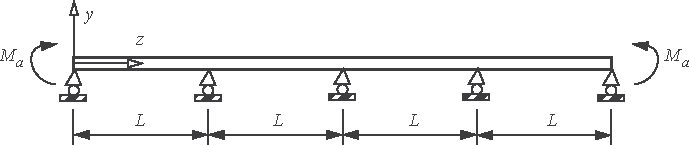
\includegraphics{Figure_16-12.pdf}
}{\caption{Multi-span beam.}\label{fig16.12}}

\subsubsection{Solution for the unknown joint displacements.} The joints are taken at the support locations and are numbered one to five from left to right. Hence, there are ten degrees of freedom (DOFs) as is shown in the top sketch in figure~\ref{fig16.13}. The support conditions mean the vertical displacements vanish; i.e.,
\begin{align}\label{eq16.6a}\tag{a}
\left\{q_{\beta}\right\}=\left[\begin{array}{@{}l@{\;}l@{\;}l@{\;}l@{\;}l@{}}q_{1} & q_{3} & q_{5} & q_{7} & q_{9}\end{array}\right]^{T}=0_{5X1}.
\end{align}
The geometry, boundary conditions, and material properties of the structure are symmetric about the vertical centerline. If the top sketch of the beam and its DOFs are rotated $180^{\circ}$ about this vertical centerline, the bottom sketch is obtained. See figure~\ref{fig16.13}. The displacements and rotations at the joints in the top and bottom sketch must be the same. Hence, symmetry implies the joint rotations must satisfy

\begin{figure}
\centerline{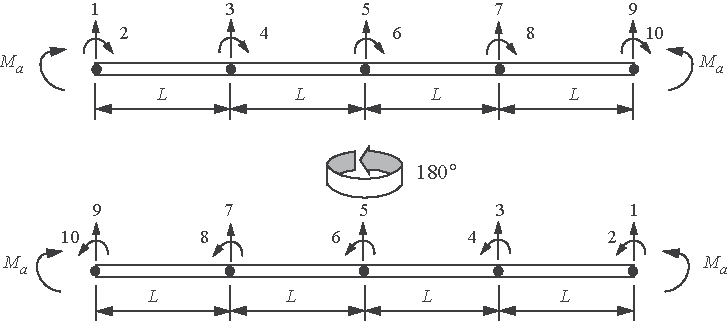
\includegraphics{Figure_16-13.pdf}}
\caption{Symmetry about midspan.}\label{fig16.13}
\end{figure}

\vspace*{-2pc}

\begin{align}\label{eq16.6b}\tag{b}
q_{10}=-q_{2} \quad q_{8}=-q_{4} \quad q_{6}=-q_{6}.
\end{align}
\noindent Clearly, the last symmetry condition on the rotations means rotation of the center joint vanishes; $q_{6}=0$. Then, the analysis for the response of the beam reduces to a two-span beam, clamped at its right end as is shown in figure~\ref{fig16.14}. The two active degrees of freedom are rotations $q_{2}$ and $q_{4}$. The stiffness matrices (\ref{eq16.49}) for beam members 1-2 and 2-3 are

\processfigure[!h]{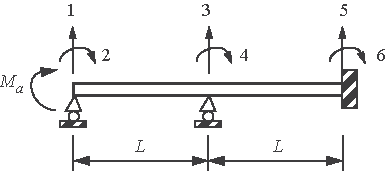
\includegraphics{Figure_16-14.pdf}
}{\caption{Equivalent two-span beam model.}\label{fig16.14}}

\vspace*{-1.8pc}

\begin{align}\label{eq16.6c}\tag{c}
\left[K_{1-2}\right]=E I
\begin{array}{@{}c@{}}
{\arraycolsep=13pt\begin{array}{@{}cccc@{}}
q_1 & q_2 & q_3 & q_4
\end{array}}\\[6pt]
\left[\begin{array}{@{}cccc@{}}12 / L^{3} & -6 / L^{2} & -12 / L^{3} & -6 / L^{2} \\-6 / L^{2} & 4 / L & 6 / L^{2} & 2 / L \\-12 / L^{3} & 6 / L^{2} & 12 / L^{3} & 6 / L^{2} \\
-6 / L^{2} & 2 / L & 6 / L^{2} & 4 / L\end{array}\right]
\end{array}
\left[K_{2-3}\right]=E I
\begin{array}{@{}c@{}}
{\arraycolsep=13pt\begin{array}{@{}cccc@{}}
q_3 & q_4 & q_5 & q_6
\end{array}}\\[6pt]
\left[\begin{array}{@{}cccc@{}}12 / L^{3} & -6 / L^{2} & -12 / L^{3} & -6 / L^{2} \\-6 / L^{2} & 4 / L & 6 / L^{2} & 2 / L \\-12 / L^{3} & 6 / L^{2} & 12 / L^{3} & 6 / L^{2} \\-6 / L^{2} & 2 / L & 6 / L^{2} & 4 / L\end{array}\right]
\end{array}.
\end{align}
The 6X6 unrestrained structural stiffness matrix is the sum $\left[K_{1-2}\right]+\left[K_{2-3}\right]$ with each member stiffness matrix expanded to 6X6 by adding two rows and two columns of zeros for degrees of freedom not contained in the member. The result is
\begin{align}\label{eq16.6d}\tag{d}
[K]=E I
\begin{array}{@{}c@{}}
{\arraycolsep=15pt\begin{array}{@{}cccccc@{}}
q_1 & q_2 & q_3 & q_4 & q_5 & q_6
\end{array}}\\[6pt]
\left[\begin{array}{@{}cccccc@{}}12 / L^{3} & -6 / L^{2} & -12 / L^{3} & -6 / L^{2} & 0 & 0 \\-6 / L^{2} & 4 / L & 6 / L^{2} & 2 / L & 0 & 0 \\-12 / L^{3} & 6 / L^{2} & 24 / L^{3} & 0 & -12 / L^{3} & -6 / L^{2} \\-6 / L^{2} & 2 / L & 0 & 8 / L & 6 / L^{2} & 2 / L \\0 & 0 & -12 / L^{3} & 6 / L^{2} & 12 / L^{3} & 6 / L^{2} \\0 & 0 & -6 / L^{2} & 2 / L & 6 / L^{2} & 4 / L\end{array}\right]
\end{array}.
\end{align}
Partition the unrestrained structural stiffness matrix in terms of unknowns and knowns to get
\begin{align}\label{eq16.6e}\tag{e}
[K]=E I
\begin{array}{@{}c@{}}
{\arraycolsep=15pt\begin{array}{@{}cccccc@{}}
q_2 & q_4 & q_1 & q_3 & q_5 & q_6
\end{array}}\\[6pt]
\left[\begin{array}{cc:cccc}4 / L & 2 / L & -6 / L^{2} & 6 / L^{2} & 0 & 0 \\2 / L & 8 / L & -6 / L^{2} & 0 & 6 / L^{2} & 2 / L \\\hdashline-6 / L^{2} & -6 / L^{2} & 12 / L^{3} & -12 / L^{3} & 0 & 0 \\6 / L^{3} & 0 & -12 / L^{3} & 24 / L^{3} & -12 / L^{3} & -6 / L^{2} \\0 & 6 / L^{2} & 0 & -12 / L^{3} & 12 / L^{3} & 6 / L^{2} \\0 & 2 / L & 0 & -6 / L^{2} & 6 / L^{2} & 4 / L\end{array}\right]
\end{array}
=\left[\begin{array}{@{}l@{}}{\left[K_{\alpha \alpha}\right]\left[K_{\alpha \beta}\right]} \\{\left[K_{\beta \alpha}\right]\left[K_{\beta \beta}\right]}\end{array}\right].
\end{align}
The restrained structural stiffness matrix is
\begin{align}\label{eq16.6f}\tag{f}
\left[K_{\alpha \alpha}\right]=E I
\begin{array}{@{}c@{}}
{\arraycolsep=12pt\begin{array}{@{}cc@{}}q_{2} &q_{4}\end{array}} \\[3pt]\left[\begin{array}{@{}cc@{}}4 / L & 2 / L \\2 / L & 8 / L\end{array}\right]\end{array}.
\end{align}
The unknown rotations are determined from
\begin{align}\label{eq16.6g}\tag{g}
\left[\begin{array}{@{}c@{}}Q_{2} \\Q_{4}\end{array}\right]=\left[\begin{array}{@{}c@{}}M_{a} \\0\end{array}\right]=E I\left[\begin{array}{@{}ll@{}}4 / L & 2 / L \\2 / L & 8 / L\end{array}\right]\left[\begin{array}{@{}l@{}}q_{2} \\q_{4}\end{array}\right].
\end{align}
Solve eq. (\textbf{\ref{eq16.6g}}) for the nodal rotations to find
\begin{align}\label{eq16.6h}\tag{h}
\left[\begin{array}{@{}l@{}}q_{2} \\q_{4}\end{array}\right]=\frac{L}{E I} \frac{1}{(32-4)}\left[\begin{array}{@{}cc@{}}8 & -2 \\-2 & 4\end{array}\right]\left[\begin{array}{@{}c@{}}M_{a} \\0\end{array}\right]=\frac{M_{a} L}{14 E I}\left[\begin{array}{@{}c@{}}4 \\-1\end{array}\right].
\end{align}
By symmetry the joint rotations for the entire structure are
\begin{align}\label{eq16.6i}\tag{i}
\left[\begin{array}{@{}c@{}}q_{2} \\q_{4} \\q_{6} \\q_{8} \\q_{10}\end{array}\right]=\frac{M_{a} L}{14 E I}\left[\begin{array}{@{}c@{}}4 \\-1 \\0 \\1 \\-4\end{array}\right].
\end{align}
\subsubsection{Solution for the shear force and bending moment distributions.} The shear force and bending moment distribution in beam members 1-2 and 2-3 are determined from eq.~(\ref{eq16.44}). For member 1-2, we have
\begin{align}\label{eq16.6j}\tag{j}
\left[\begin{array}{@{}l@{}}V_{1}(z) \\M_{1}(z)\end{array}\right]_{1-2}=E I\left[\begin{array}{@{}cccc@{}}-\frac{12}{L^{3}} & \frac{6}{L^{2}} & \frac{12}{L^{3}} & \frac{6}{L^{2}} \\\left(\frac{6}{L^{2}}-\frac{12 z}{L^{3}}\right) & \left(-\frac{4}{L}+\frac{6 z}{L^{2}}\right) & \left(-\frac{6}{L^{2}}+\frac{12 z}{L^{3}}\right) & \left(-\frac{2}{L}+\frac{6 z}{L^{2}}\right)\end{array}\right]\left[\begin{array}{@{}l@{}}q_{1} \\q_{2} \\q_{3} \\q_{4}\end{array}\right].
\end{align}
But $q_{1}=q_{3}=0$, so
\begin{align}\label{eq16.6k}\tag{k}
\left[\begin{array}{@{}l@{}}V_{1}(z) \\M_{1}(z)\end{array}\right]_{1-2}=E I\left[\begin{array}{@{}cc@{}}\frac{6}{L^{2}} & \frac{6}{L^{2}} \\[6pt]\left(-\frac{4}{L}+\frac{6 z}{L^{2}}\right)&\left(-\frac{2}{L}+\frac{6 z}{L^{2}}\right)\end{array}\right]\left[\begin{array}{@{}l@{}}q_{2} \\q_{4}\end{array}\right].
\end{align}
Substitute the solution for the rotations from eq. (\textbf{\ref{eq16.6h}}) into eq. (\textbf{\ref{eq16.6k}}) to get
\begin{align}\label{eq16.6l}\tag{l}
\left[\begin{array}{@{}l@{}}V_{1}(z) \\M_{1}(z)\end{array}\right]_{1-2}=E I\left[\begin{array}{@{}cc@{}}\frac{6}{L^{2}} & \frac{6}{L^{2}} \\\left(-\frac{4}{L}+\frac{6 z}{L^{2}}\right)&\left(-\frac{2}{L}+\frac{6 z}{L^{2}}\right)\end{array}\right] \frac{M_{a} L}{14 E I}\left[\begin{array}{@{}c@{}}4 \\-1\end{array}\right]=\frac{M_{a} L}{14}\left[\begin{array}{@{}c@{}}\frac{18}{L^{2}} \\-\frac{14}{L}+18 \frac{z}{L^{2}}\end{array}\right]=\left[\begin{array}{@{}c@{}}\frac{9 M_{a}}{7 L} \\-M_{a}+\frac{9 M_{a}}{7 L }z\end{array}\right].
\end{align}
\textit{Note that the coordinate z is local to the member in the formulas for the shear force and bending moment}. For member 2-3, we have\vspace*{-2pc}

\processfigure[!b]{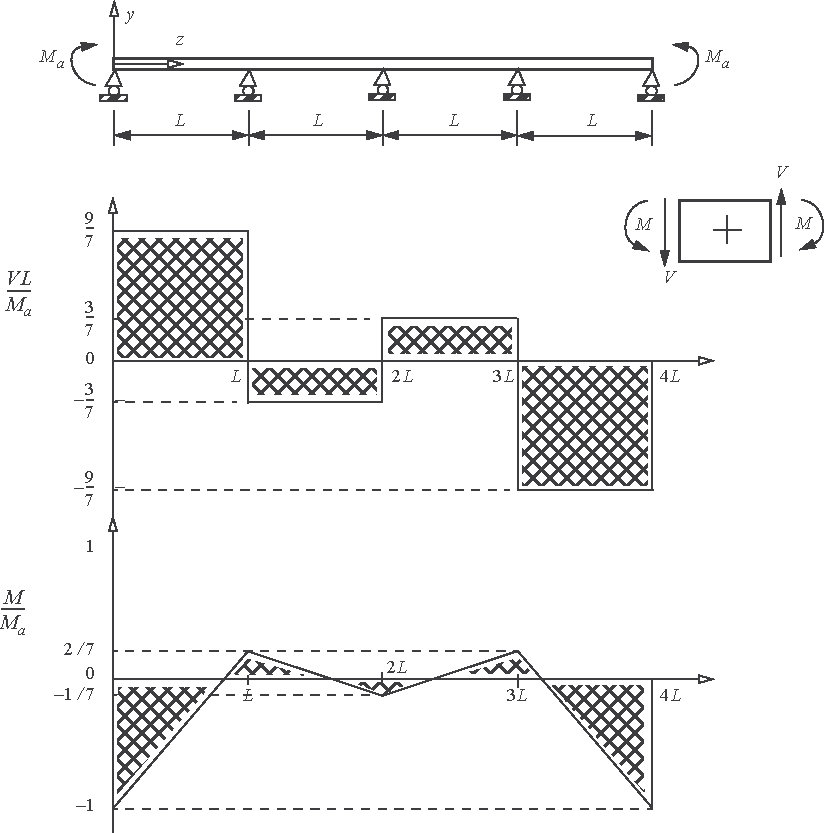
\includegraphics{Figure_16-15.pdf}
}{\caption{Shear force and bending moment diagrams for the multispan beam.}\label{fig16.15}}

\begin{align}\label{eq16.6m}\tag{m}
\left[\begin{array}{@{}l@{}}V_{1}(z) \\M_{1}(z)\end{array}\right]_{2-3}=E I\left[\begin{array}{@{}cccc@{}}-\frac{12}{L^{3}} & \frac{6}{L^{2}} & \frac{12}{L^{3}} & \frac{6}{L^{2}} \\[6pt]\frac{6}{L^{2}}-\frac{12 z}{L^{3}} & -\frac{4}{L}+\frac{6 z}{L^{2}} & -\frac{6}{L^{2}}+\frac{12 z}{L^{3}} & -\frac{2}{L}+\frac{6 z}{L^{2}}\end{array}\right]\left[\begin{array}{@{}l@{}}q_{3} \\q_{4} \\q_{5} \\q_{6}\end{array}\right].
\end{align}
But $q_{3}=q_{5}=q_{6}=0$, so
\begin{align}\label{eq16.6n}\tag{n}
\left[\begin{array}{@{}l@{}}V_{1}(z) \\M_{1}(z)\end{array}\right]_{2-3}=E I\left[\begin{array}{@{}c@{}}\frac{6}{L^{2}} \\[6pt]-\frac{4}{L}+\frac{6 z}{L^{2}}\end{array}\right] q_{4}.
\end{align}
Substitute the solution for rotation $q_{4}$ from eq. (\textbf{\ref{eq16.6h}}) into eq. (\textbf{\ref{eq16.6n}}) to get
\begin{align}\label{eq16.6o}\tag{o}
\left[\begin{array}{@{}l@{}}V_{1}(z) \\M_{1}(z)\end{array}\right]_{2-3}=E I\left[\begin{array}{@{}c@{}}\frac{6}{L^{2}} \\[6pt]-\frac{4}{L}+\frac{6 z}{L^{2}}\end{array}\right]\left(-\frac{M_{a} L}{14 E I}\right)=\left[\begin{array}{@{}c@{}}-\frac{3 M_{a}}{7 L} \\[6pt]\frac{2 M_{a}}{7}-\frac{3 M_{a}}{7 L} z\end{array}\right].
\end{align}
Again, note that the $z$-coordinate in these formulas for the shear force and bending moment in member 2-3 is local to the member and runs from zero to \textit{L}. However, the beginning joint 2 corresponds to the global longitudinal coordinate \textit{L}, and end joint 3 corresponds to the global longitudinal coordinate 2\textit{L}. The relationship between the member local coordinate and the global structural coordinate has to be taken into account when drawing the shear force and bending moment diagrams. The shear force and bending moment diagrams are shown in figure~\ref{fig16.15}. In this example, the shear force diagram in antisymmetric, and the moment diagram is symmetric, about the center of the multispan beam.


\subsubsection{Solution for the support reactions.} The support reactions are $\left[Q_{\beta}\right]=\left[K_{\beta \alpha}\right]\left\{q_{\alpha}\right\}$, since $\left\{q_{\beta}\right\}=0_{4 X 1}$. Hence,
\begin{align}\label{eq16.6p}\tag{p}
\left[\begin{array}{@{}l@{}}Q_{1} \\Q_{3} \\Q_{5} \\O_{6}\end{array}\right]=E I\left[\begin{array}{@{}cc@{}}-6 / L^{2} & -6 / L^{2} \\6 / L^{2} & 0 \\0 & 6 / L^{2} \\0 & 2 / L\end{array}\right]\left[\begin{array}{@{}l@{}}q_{2} \\q_{4}\end{array}\right]=E I\left[\begin{array}{@{}cc@{}}-6 / L^{2} & -6 / L^{2} \\6 / L^{2} & 0 \\0 & 6 / L^{2} \\0 & 2 / L\end{array}\right] \frac{M_{a} L}{14 E I}\left[\begin{array}{@{}c@{}}4 \\-1\end{array}\right]=M_{a}\left[\begin{array}{@{}c@{}}-9 /(7 L) \\12 /(7 L) \\-3 /(7 L) \\-1 / 7\end{array}\right].
\end{align}
Note that these are the support reactions for the left half of the beam. By symmetry the support reactions on the right half of the beam are obtained by a rotation of the left half by $180^{\circ}$ as shown in figure~\ref{fig16.16}.

\begin{figure}[!h]
\centerline{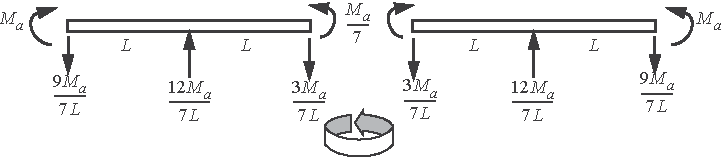
\includegraphics{Figure_16-16.pdf}}
\caption{Support reactions from the half models of the multispan beam.}\label{fig16.16}
\end{figure}

Joining the left half and right half we get the support reactions for the overall free body diagram of the multispan beam as shown in figure~\ref{fig16.17}.
\end{example}

\begin{figure}[!h]
\centerline{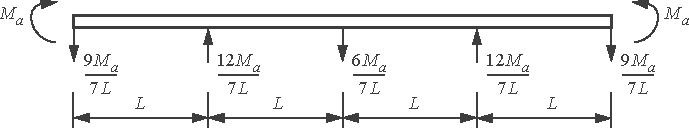
\includegraphics{Figure_16-17.pdf}}
\caption{Support reactions of the intact multispan beam.}\label{fig16.17}
\end{figure}

\begin{example*}[Clamped-clamped, stepped beam restrained by a spring]\label{ex16.7}The beam structure shown in figure~\ref{fig16.18}(a) has a step change in thickness at midspan, and is clamped at each end. The left half of has a uniform flexural stiffness $2 E I$, and the right half has a uniform flexural stiffness $E I$. Each half has a length denoted by $a$. A vertical linear elastic spring of stiffness $k=6 E I / a^{3}$ is connected at midspan. The structure is subject to a vertical distributed load and a vertical point force $P$ applied at midspan. The distributed load is uniform on the left half with intensity $f_{y 0}$, and decreases linearly from $f_{y 0}$ to zero on the right half. Model the response of the beam with two beam members, one in each half, and a spring member. Determine\pagebreak

\begin{enumerate}
\item[a)] The restrained structural stiffness matrix.

\item[b)] The fixed-end action vector.

\item[c)] The unknown joint displacements.

\item[d)] The support reactions.

\item[e)] The shear force and bending moment in the left half of the beam.
\end{enumerate}

\processfigure[!h]{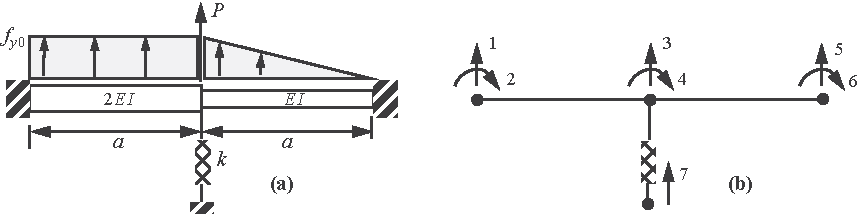
\includegraphics{Figure_16-18.pdf}
}{\caption{(a) Beam with a step change in thickness. (b) Degree of freedom numbering.}\label{fig16.18}}

%\vspace*{-1pc}

\subsubsection{Solution to part (a).} The unrestrained structure has four joints and seven degrees of freedom as shown in figure~\ref{fig16.18}(b). The size of the unrestrained structural stiffness matrix is 7X7. The support conditions impose the vanishing of the following generalized displacement vector: $\left\{q_{\beta}\right\}=\left[\begin{array}{@{}l@{\;}l@{\;}l@{\;}l@{\;}l@{}}q_{1} & q_{2} & q_{5} & q_{6} & q_{7}\end{array}\right]^{T}=0_{5X1}$. The active, or unknown, displacement vector is $\left\{q_{\alpha}\right\}=\left[\begin{array}{@{}l@{\;}l@{}}q_{3} & q_{4}\end{array}\right]^{T}$.

The stiffness matrices for the two beam members are obtained from eq.~(\ref{eq16.49}) as
\begin{align}\label{eq16.7a}\tag{a}
\left[K_{1-2}\right]=E I
\begin{array}{@{}c@{}}
{\arraycolsep=13pt\begin{array}{@{}cccc@{}}
q_1 & q_2 & q_3 & q_4
\end{array}}\\[6pt]
\left[\begin{array}{@{}cccc@{}}24 / a^{3} & -12 / a^{2} & -24 / a^{3} & -12 / a^{2} \\-12 / a^{2} & 8 / a & 12 / a^{2} & 4 / a \\-24 / a^{3} & 12 / a^{2} & 24 / a^{3} & 12 / a^{2} \\-12 / a^{2} & 4 / a & 12 / a^{2} & 8 / a\end{array}\right]
\end{array}
\left[K_{2-3}\right]=E I
\begin{array}{@{}c@{}}
{\arraycolsep=13pt\begin{array}{@{}cccc@{}}
q_3 & q_4 & q_5 & q_6
\end{array}}\\[6pt]
\left[\begin{array}{@{}cccc@{}}12 / a^{3} & -6 / a^{2} & -12 / a^{3} & -6 / a^{2} \\-6 / a^{2} & 4 / a & 6 / a^{2} & 2 / a \\-12 / a^{3} & 6 / a^{2} & 12 / a^{3} & 6 / a^{2} \\-6 / a^{2} & 2 / a & 6 / a^{2} & 4 / a\end{array}\right]
\end{array}.
\end{align}
The spring stiffness matrix is obtained from eq.~(\ref{eq15.8}) on page~\pageref{eq15.8} as
\begin{align}\label{eq16.7b}\tag{b}
\left[K_{4-2}\right]=E I
\begin{array}{@{}c@{}}
{\arraycolsep=13pt\begin{array}{@{}cc@{}}
q_7 & q_3
\end{array}}\\[6pt]
\left[\begin{array}{@{}cc@{}}6 / a^{3} & -6 / a^{3} \\-6 / a^{3} & 6 / a^{3}\end{array}\right]
\end{array}.
\end{align}
Assembly of the element stiffness matrices is by summation of the element stiffness matrices with attention to the location of the matrix elements in the 7X7 unrestrained structural stiffness matrix. The result is
\begin{align}\label{eq16.7c}\tag{c}
[K]=E I
\begin{array}{@{}c@{}}
{\arraycolsep=15pt\begin{array}{@{}ccccccc@{}}
q_1 & q_2 & q_3 & q_4 & q_5 & q_6 & q_7
\end{array}}\\[6pt]
\left[\begin{array}{@{}ccccccc@{}}24 / a^{3} & -12 / a^{2} & -24 / a^{3} & -12 / a^{2} & 0 & 0 & 0 \\-12 / a^{2} & 8 / a & 12 / a^{2} & 4 / a & 0 & 0 & 0 \\-24 / a^{3} & 12 / a^{2} & 42 / a^{3} & 6 / a^{2} & 12 / a^{3} & -6 / a^{2} & -6 / a^{3} \\-12 / a^{2} & 4 / a & 6 / a^{2} & 12 / a & 6 / a^{2} & 2 / a & 0 \\0 & 0 & -12 / a^{3} & 6 / a^{2} & 12 / a^{3} & 6 / a^{2} & 0 \\0 & 0 & -6 / a^{2} & 2 / a & 6 / a^{2} & 4 / a & 0 \\0 & 0 & -6 / a^{3} & 0 & 0 & 0 & 6 / a^{3}\end{array}\right]
\end{array}.
\end{align}
Partition the unrestrained structural stiffness matrix in eq. (\ref{eq16.7c}) so that rows and columns are in the order 3, 4, 1, 2, 5, 6, 7:
\begin{align}\label{eq16.7d}\tag{d}
[K]=E I
\begin{array}{@{}c@{}}
{\arraycolsep=16pt\begin{array}{@{}ccccccc@{}}
q_3 & q_4 & q_1 & q_2 & q_5 & q_6 & q_7
\end{array}}\\[6pt]
\left[\begin{array}{cc;{2pt/2pt}ccccc}42 / a^{3} & 6 / a^{2} & -24 / a^{3} & 12 / a^{2} & -12 / a^{3} & -6 / a^{2} & -6 / a^{3} \\6 / a^{2} & 12 / a & -12 / a^{2} & 4 / a & 6 / a^{2} & 2 / a & 0 \\\hdashline[2pt/2pt] -24/ a^{3} & -12 / a^{2} & 24 / a^{3} & -12 / a^{2} & 0 & 0 & 0 \\12 / a^{2} & 4 / a & -12 / a^{2} & 8 / a & 0 & 0 & 0 \\-12 / a^{3} & 6 / a^{2} & 0 & 0 & 12 / a^{3} & 6 / a^{2} & 0 \\-6 / a^{2} & 2 / a & 0 & 0 & 6 / a^{2} & 4 / a & 0 \\-6 / a^{3} & 0 & 0 & 0 & 0 & 0 & 6 / a^{3}\end{array}\right]
\end{array}
=\left[\begin{array}{@{}ll@{}}{\left[K_{\alpha \alpha}\right]} & {\left[K_{\alpha \beta}\right]} \\{\left[K_{\beta \alpha}\right]} & {\left[K_{\beta \beta}\right]}\end{array}\right].
\end{align}
From the partitioned form of eq. (\ref{eq16.7d}) the restrained structural stiffness matrix is
\begin{align}\label{eq16.7e}\tag{e}
\left[K_{\alpha \alpha}\right]=E I\left[\begin{array}{@{}cc@{}}42 / a^{3} & 6 / a^{2} \\6 / a^{2} & 12 / a\end{array}\right].
\end{align}

\vspace*{-1pc}

\subsubsection{Solution to part (b).} From eqs. (\ref{eq16.54}) and (\ref{eq16.56}) fixed-end actions of the beam member are
\begin{align}\label{eq16.7f}\tag{f}
\left[\begin{array}{@{}l@{}}Q_{1}^{0} \\[6pt]Q_{2}^{0} \\[6pt]Q_{3}^{0} \\[6pt]Q_{4}^{0}\end{array}\right]_{1-2}=\left[\begin{array}{@{}c@{}}-a f_{y 0} / 2 \\[3pt]a^{2} f_{y 0} / 12 \\[3pt]-a f_{y 0} / 2 \\[3pt]-a^{2} f_{y 0} / 12\end{array}\right]\left[\begin{array}{@{}l@{}}Q_{3}^{0} \\[6pt]Q_{4}^{0} \\[6pt]Q_{5}^{0} \\[6pt]Q_{6}^{0}\end{array}\right]_{2-3}=\left[\begin{array}{@{}c@{}}-7 a f_{y 0} / 20 \\[3pt]a^{2} f_{y 0} / 20 \\[3pt]-3 a f_{y 0} / 20 \\[3pt]-a^{2} f_{y 0} / 30\end{array}\right].
\end{align}
The assembled 7X1 fixed-end action vector in the natural order 1, 2, 3, 4, 5, 6, 7 is
\[
\left\{Q^{0}\right\}=\left[\frac{-a}{2} \frac{a^{2}}{12} \frac{-17 a}{20} \frac{-a^{2}}{30} \frac{-3 a}{20} \frac{-a^{2}}{30} 0\right]^{T} f_{y 0}.
\]
Partitioning the fixed-end action vector in the order 3, 4, 1, 2, 5, 6, 7 we get
\[
\left\{Q^{0}\right\}=\left[\frac{-17 a}{20} \frac{-a^{2}}{30} \bigg| \frac{-a}{2} \frac{a^{2}}{12} \frac{-3 a}{20} \frac{-a^{2}}{30} 0\right]^{T} f_{y 0}=\left\{Q_{\alpha}^{0}\right\}+\left\{Q_{\beta}^{0}\right\},
\]
where
\begin{align}\label{eq16.7g}\tag{g}
\left\{Q_{\alpha}^{0}\right\}=\left[\frac{-17 a}{20} \frac{-a^{2}}{30}\right]^{T} f_{y 0} \quad\left\{Q_{\beta}^{0}\right\}=\left[\frac{-a}{2} \frac{a^{2}}{12} \frac{-3 a}{20} \frac{-a^{2}}{30} 0\right]^{T} f_{y 0}.
\end{align}

\vspace*{-1pc}

\subsubsection{Solution to part (c).} The matrix equation to determine the unknown joint displacement $\left\{q_{\alpha}\right\}$ is
\begin{align}\label{eq16.7h}\tag{h}
\left\{Q_{\alpha}\right\}=\left[K_{\alpha \alpha}\right]\left\{q_{\alpha}\right\}+\left[K_{\alpha \beta}\right]\left\{q_{\beta}\right\}+\left\{Q_{\alpha}^{0}\right\}.
\end{align}
The prescribed joint force vector $\left\{Q_{\alpha}\right\}$ is
\begin{align}\label{eq16.7i}\tag{i}
\left[\begin{array}{@{}c@{}}Q_{3} \\Q_{4}\end{array}\right]_{\alpha}=\left[\begin{array}{@{}l@{}}P \\0\end{array}\right].
\end{align}
The specified displacement vector $\left\{q_{\beta}\right\}=0{ }_{5 X 1}$. The matrix equation for the solution of the displacement vector $\left\{q_{\alpha}\right\}$ reduces to\vspace*{-6pt}
\begin{align}\label{eq16.7j}\tag{j}
\left[K_{\alpha \alpha}\right]\left\{q_{\alpha}\right\}=\left\{Q_{\alpha}\right\}+(-\{Q_{\alpha}^{0}\}),
\end{align}

\processfigure[!h]{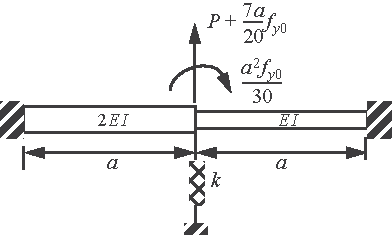
\includegraphics{Figure_16-19.pdf}
}{\caption{Applied load $P$ and the equivalent joint\break forces from the distributed loading.}\label{fig16.19}}

\vspace*{-1pc}

\noindent where $\left(-\left\{Q_{\alpha}^{0}\right\}\right)$ is the equivalent joint force vector. See figure~\ref{fig16.19}. The explicit form of the matrix equation to determine the unknown displacements is
\[
E I\left[\begin{array}{@{}cc@{}}42 / a^{3} & 6 / a^{2} \\6 / a^{2} & 12 / a\end{array}\right]\left[\begin{array}{@{}l@{}}q_{3} \\q_{4}\end{array}\right]=\left[\begin{array}{@{}c@{}}P \\0\end{array}\right]+\left[\begin{array}{@{}c@{}}17 a / 20 \\a^{2} / 30\end{array}\right] f_{y 0}.
\]
The solution for the generalized displacements is
\begin{align}\label{eq16.7k}\tag{k}
\left[\begin{array}{@{}l@{}}q_{3} \\q_{4}\end{array}\right]=\frac{1}{E I}\left[\begin{array}{@{}cc@{}}a^{3} / 39 & -a^{2} / 78 \\-a^{2} / 78 & 7 a / 78\end{array}\right]\left[\begin{array}{@{}c@{}}P+17 a f_{y 0} / 20 \\a^{2} f_{y 0} / 30\end{array}\right]=\frac{1}{39 E I}\left[\begin{array}{@{}c@{}}
a^{3}\left(P+5 a f_{y 0} / 18\right) \\
\frac{-a^{2}}{2}\left(P+37 a f_{y 0} / 60\right)
\end{array}\right].
\end{align}

\vspace*{-1pc}

\subsubsection{Solution to part (d).} The governing matrix equation for the unknown joint forces, or the support reactions, is
\begin{align}\label{eq16.7l}\tag{l}
\left\{Q_{\beta}\right\}=\left[K_{\beta \alpha}\right]\left\{q_{\alpha}\right\}+\left[K_{\beta \beta}\right]\left\{q_{\beta}\right\}+\left\{Q_{\beta}^{0}\right\}.
\end{align}
The matrix 5X2 $\left[K_{\beta \alpha}\right]$ is obtained from the partitioned form eq. (\ref{eq16.7d}). Writing eq. (\ref{eq16.7l}) in detail we have
\begin{align}\label{eq16.7m}\tag{m}
\left[\begin{array}{@{}l@{}}Q_{1} \\Q_{2} \\Q_{5} \\Q_{6} \\Q_{7}\end{array}\right]=E I\left[\begin{array}{@{}cc@{}}-24 / a^{3} & -12 / a^{2} \\12 / a^{2} & 4 / a \\-12 / a^{3} & 6 / a^{2} \\-6 / a^{2} & 2 / a \\-6 / a^{3} & 0\end{array}\right] \frac{1}{39 E I}\left[\begin{array}{@{}c@{}}a^{3} P+5 a f_{y 0} / 18 \\\frac{-a^{2}}{2} P+37 a f_{y 0} / 60\end{array}\right]+\left[\begin{array}{@{}c@{}}-a / 2 \\a^{2} / 12 \\-3 a / 20 \\-a^{2} / 30 \\0\end{array}\right] f_{y 0}.
\end{align}
After performing the matrix algebra in eq. (\ref{eq16.7m}) the result for the support reactions is
\begin{align}\label{eq16.7n}\tag{n}
\left[\begin{array}{@{}l@{}}Q_{1} \\Q_{2} \\Q_{5} \\Q_{6} \\O_{7}\end{array}\right]=\left[\begin{array}{@{}cc@{}}-6 / 13 & -179 / 195 \\10 a / 39 & 721 a / 2,340 \\-5 / 13 & -59 / 130 \\7 a / 39 & -83 a / 468 \\2 / 13 & -5 / 39\end{array}\right]\left[\begin{array}{@{}c@{}}P \\a f_{y 0}\end{array}\right].
\end{align}

\vspace*{-1.3pc}\pagebreak

\subsubsection{Solution to part e.} Referring to eq.~(\ref{eq16.61}) on page~\pageref{eq16.61}, the shear force and bending moment in beam member 1-2 is given by the superposition of the fixed-end solution and the displacement solution as
\begin{align}\label{eq16.7o}\tag{o}
\left[\begin{array}{@{}c@{}}V_{y}(z) \\M_{x}(z)\end{array}\right]_{1-2}=\left[\begin{array}{@{}c@{}}V_{y}^{0}(z) \\M_{x}^{0}(z)\end{array}\right]_{1-2}+\left[\begin{array}{@{}c@{}}V_{y}^{1}(z) \\M_{x}^{1}(z)\end{array}\right]_{1-2}=\left[\begin{array}{@{}c@{}}V_{y}^{0}(z) \\M_{x}^{0}(z)\end{array}\right]_{1-2}+\left[S^{1}(z)\right]_{1-2}\{q\}_{1-2}.
\end{align}
From the fixed-end action solution (\ref{eq16.55}) the vector of the shear force and bending moment is
\begin{align}\label{eq16.7p}\tag{p}
\left[\begin{array}{@{}c@{}}V_{y}^{0}(z) \\[3pt]M_{x}^{0}(z)\end{array}\right]_{1-2}=\left[\begin{array}{@{}c@{}}(a-2 z) / 2 \\\left(-a^{2}+6 a z-6 z^{2}\right) / 12\end{array}\right] f_{y 0} \quad 0 \leq z \leq a.
\end{align}
Equations (\ref{eq16.45}) and (\ref{eq16.46}) combine to determine the shear and moment from the displacements of the member. That is,
\begin{align}\label{eq16.7q}\tag{q}
\left[\begin{array}{@{}c@{}}V_{y}^{1}(z) \\[3pt]M_{x}^{1}(z)\end{array}\right]_{1-2}=\left[S^{1}(z)\right]_{1-2}\left[\begin{array}{@{}l@{}}q_{1} \\q_{2} \\q_{3} \\q_{4}\end{array}\right]=E I\left[\begin{array}{c:c:c:c}-\frac{12}{a^{3}} & \frac{6}{a^{2}} & \frac{12}{a^{3}} & \frac{6}{a^{2}} \\[6pt]\frac{6}{a^{2}}-\frac{12 z}{a^{3}} & -\frac{4}{a}+\frac{6 z}{a^{2}} & -\frac{6}{a^{2}}+\frac{12 z}{a^{3}} & -\frac{2}{a}+\frac{6 z}{a^{2}}\end{array}\right]\left[\begin{array}{@{}c@{}}0 \\0 \\q_{3} \\q_{4}\end{array}\right].
\end{align}
Perform the matrix algebra in eq. (\textbf{\ref{eq16.7q}}) to find
\begin{align}\label{eq16.7r}\tag{r}
\left[\begin{array}{@{}c@{}}V_{y}^{1}(z) \\[3pt]M_{x}^{1}(z)\end{array}\right]_{1-2}=E I\left[\begin{array}{@{}cc@{}}\frac{12}{a^{3}} & \frac{6}{a^{2}} \\[6pt]-\frac{6}{a^{2}}+\frac{12 z}{a^{3}} &-\frac{2}{a}+\frac{6 z}{a^{2}}\end{array}\right] \frac{1}{39 E I}\left[\begin{array}{@{}c@{}}a^{3} P+5 a f_{y 0} / 18 \\-\frac{a^{2}}{2} P+37 a f_{y 0} / 60\end{array}\right]=\left[\begin{array}{@{}cc@{}}\frac{6}{13} &\frac{163a}{390}\\[6pt]
\left(\frac{-10 a}{39}+\frac{6 z}{13}\right)&\left(\frac{-263 a^{2}}{1170}+\frac{163 a z}{390}\right)\end{array}\right]\left[\begin{array}{@{}c@{}}P \\f_{y 0}\end{array}\right].
\end{align}
Finally, substitute eqs. (\textbf{\ref{eq16.7p}}) and (\textbf{\ref{eq16.7r}}) into (\textbf{\ref{eq16.7o}}) to get
\begin{align*}
\left[\begin{array}{@{}l@{}}V_{y}(z) \\[3pt]M_{x}(z)\end{array}\right]_{1-2}=\left[\begin{array}{@{}cc@{}}\frac{6}{13} & \frac{179 a}{195}-z \\[3pt]\left(\frac{-10 a}{39}+\frac{6 z}{13}\right)&\left(\frac{-721 a^{2}}{2,340}+\frac{179 a z}{195}-\frac{z^{2}}{2}\right)\end{array}\right]\left[\begin{array}{@{}c@{}}P \\f_{y 0}\end{array}\right] \quad 0 \leq z \leq a. \\[-2.5pc]
\text{\hfill\qed\hspace*{-83pt}}
\end{align*}
\end{example*}

\vspace*{-1pc}

\section{Coplanar frame structures}\label{sec16.3}

Frame members in a skeletal structure resist applied loads both by axial deformation and bending deformation. Frames are often modeled by assuming the joints are rigid, which means that members meeting at a joint have the same rotation. That is, instead of frictionless pins or ball and socket joints used to model trusses, the connections at a joint under the rigid joint assumption implies that bending moments in the members at the joint do not vanish. When distributed lateral loads act on the member, frame elements may be required even if the joints at the end of the member are modeled as frictionless pins. In a truss the loads are assumed to only act on the joints, and the members are not subject to lateral distributed loads. The stiffness matrix for a frame member is the superposition of the stiffness matrix for a truss member and the stiffness matrix for a beam member. There are three degrees of freedom at each joint in a coplanar frame member: two displacements and a rotation as shown in figure~\ref{fig16.20}. In this figure, degrees of freedom labeled one and four account for axial deformation, degrees of freedom two and five account for lateral deformation in bending, and degrees of freedom three and six account for rotations in bending. These degrees of freedom are referred to Cartesian coordinate directions along the longitudinal axis and the axis perpendicular to the member. Let the coordinate along the longitudinal, centroidal axis be denoted by $z$, $0 \leq z \leq L$, and let $y$ be the coordinate perpendicular to the member.

\begin{figure}[!h]
\centerline{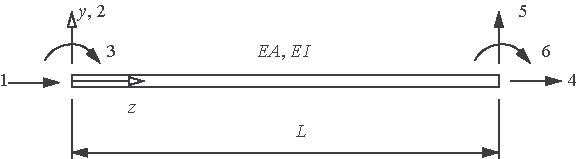
\includegraphics{Figure_16-20.pdf}}
\caption{Frame member with six degrees of freedom.}\label{fig16.20}
\end{figure}

Consider a typical plane frame member between joints $i$ and $j$ in a structure. Joint $i$ is the beginning joint and joint $j$ is the end joint, so that the $z$-axis is directed from joint $i$ to joint $j$. Then, the 6X1 generalized displacement vector for the frame member in local coordinate directions is uniquely numbered by
\begin{align}\label{eq16.62}
\{\bar{q}\}=\left[\bar{q}_{3 i-2}\ \bar{q}_{3 i-1}\ \bar{q}_{3 i}\ \bar{q}_{3 j-2}\right.\left.\bar{q}_{3 j-1}\ \bar{q}_{3 j}\right]^{T}.
\end{align}
\noindent These displacement components are shown in figure~\ref{fig16.21}. The 6X6 frame stiffness matrix in local coordinate directions is the sum of the truss stiffness matrix and the beam stiffness matrix, where

\begin{figure}[!h]
\centerline{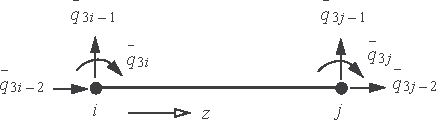
\includegraphics{Figure_16-21.pdf}}
\caption{Generalized displacements for a frame element between joints $i$ and $j$.}\label{fig16.21}
\end{figure}

\vspace*{-1.25pc}

\begin{align}\label{eq16.63}
\left[K_{\text {truss }}\right]=
\begin{array}{@{}c@{}}
{\arraycolsep=12pt\begin{array}{@{}c@{}}
\bar{q}_{3 i-2}\phantom{00000} \bar{q}_{3 j-2}\phantom{00000000}\end{array}}\\[6pt]
\left[\begin{array}{@{}cc@{}}
E A / L & -E A / L \\
-E A / L & E A / L\end{array}\right] \quad
\left[K_{{\rm beam }}\right]\end{array}=
\begin{array}{@{}c@{}}
{\arraycolsep=15pt\begin{array}{@{}cccc@{}}
\bar{q}_{3i-1} & \bar{q}_{3i} & \bar{q}_{3j-1}& \bar{q}_{3j}
\end{array}}\\[6pt]
\left[\begin{array}{@{}cccc@{}}12 E I / L^{3} & -6 E I / L^{2} & -12 E I / L^{3} & -6 E I / L^{2} \\-6 E I / L^{2} & 4 E I / L & 6 E I / L^{2} & 2 E I / L \\-12 E I / L^{3} & 6 E I / L^{2} & 12 E I / L^{3} & 6 E I / L^{2} \\-6 E I / L^{2} & 2 E I / L & 6 E I / L^{2} & 4 E I / L\end{array}\right]\end{array}.
\end{align}
Now add the stiffness matrices in eq.~(\ref{eq16.63}) with due regard to the element locations in the 6X6 frame member stiffness matrix to get
\begin{align}\label{eq16.64}
[\bar{K}]=
\begin{array}{@{}c@{}}
{\arraycolsep=15pt\begin{array}{@{}cccccc@{}}
\bar{q}_{3i-2} &\bar{q}_{3i-1} &\bar{q}_{3i} &\bar{q}_{3j-2}& \bar{q}_{3j-1}& \bar{q}_{3j}
\end{array}}\\[6pt]
\left[\begin{array}{@{}cccccc@{}}E A / L & 0 & 0 & -E A / L & 0 & 0 \\0 & 12 E I / L^{3} & -6 E I / L^{2} & 0 & -12 E I / L^{3} & -6 E I / L^{2} \\0 & -6 E I / L^{2} & 4 E I / L & 0 & 6 E I / L^{2} & 2 E I / L \\-E A / L & 0 & 0 & E A / L & 0 & 0 \\0 & -12 E I / L^{3} & 6 E I / L^{2} & 0 & 12 E I / L^{3} & 6 E I / L^{2} \\0 & -6 E I / L^{2} & 2 E I / L & 0 & 6 E I / L^{2} & 4 E I / L\end{array}\right]\end{array}.
\end{align}
The frame member stiffness matrix (\ref{eq16.64}) is symmetric, singular, and its diagonal elements are positive. Let the 6X1 generalized joint force vector corresponding to the generalized displacement vector for the member in local coordinates be denoted by
\begin{align}\label{eq16.65}
\{\bar{Q}\}=\left[\bar{Q}_{3 i-2}\;\; \bar{Q}_{3 i-1}\;\; \bar{Q}_{3 i}\;\; \bar{Q}_{3 j-2}\;\; \bar{Q}_{3 j-1}\;\; \bar{Q}_{3j}\right]^{T}.
\end{align}
Then, the matrix relationship between the generalized force and displacement vectors is
\begin{equation}\label{eq16.66}
\begin{aligned}&\{\bar{Q}\}=[\bar{K}]\{\bar{q}\} \\&6 X 1 \quad 6 X 6\ 6 X 1,\end{aligned}
\end{equation}
where the frame member stiffness matrix in local coordinate directions is given by eq.~(\ref{eq16.64}).

\subsection{Transformation of Cartesian coordinates}\label{sec16.3.1}

Let a coplanar frame assembly be defined with respect to global Cartesian coordinate directions $(X,Y,Z)$. The local Cartesian coordinates of a frame member are $(z, y, x)$ with the $z$-coordinate along the reference axis of the member. The $z$-axis lies in the \textit{X-Y} plane at an angle $\theta$ with respect to the positive \textit{X}-direction as shown in figure~\ref{fig16.22}. To effect the assembly of member stiffness matrices it is necessary to transform the stiffness matrix (\ref{eq16.64}) of a member from local coordinate directions $(z, y, x)$ to the global coordinate directions $(X,Y,Z)$. The transformation from one Cartesian system $(X,Y,Z)$ to another Cartesian system ($z,y,x$) at joint $i$ is effected by the direction cosines of the latter with respect to the former. For example, denote the cosine of the angle of the $z$-direction with respect to the \textit{Z}-direction as $\cos (z, Z)$ , the cosine of the angle of the $z$-direction with respect to the $Y$-direction as $\cos (z, Y)$, etc. Then the Cartesian coordinate transformation from global to local directions in terms of the direction cosines is

\processfigure[!h]{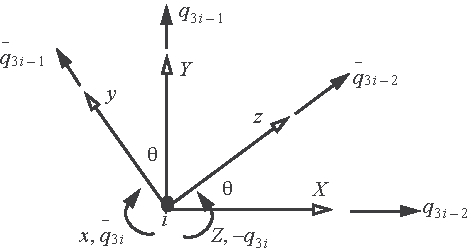
\includegraphics{Figure_16-22.pdf}
}{\caption{Local and global direction at node $i$.}\label{fig16.22}}

\vspace*{-1.25pc}

\begin{align}\label{eq16.67}
\begin{split}
z&=\cos (z, X) X+\cos (z, Y) Y+\cos (z, Z) Z \\
y&=\cos (y, X) X+\cos (y, Y) Y+\cos (y, Z) Z \\
x&=\cos (x, X) X+\cos (x, Y) Y+\cos (x, Z) Z
\end{split}.
\end{align}
From figure~\ref{fig16.22} the directions cosines in terms of angle $\theta$ are as follows.
\begin{align}
\cos (z, X)&=\cos \theta, \cos (z, Y)=\cos \left(-\theta+90^{\circ}\right)=\sin \theta, \cos (z, Z)=\cos 90^{\circ}=0\label{eq16.68}\\
\cos (y, X)&=\cos \left(\theta+90^{\circ}\right)=-\sin \theta, \cos (y, Y)=\cos \theta, \cos (y, Z)=\cos 90^{\circ}=0,\label{eq16.69}\\
\cos (x, X)&=\cos 90^{\circ}=0, \cos (x, Y)=\cos 90^{\circ}=0, \cos (x, Z)=\cos 180^{\circ}=-1.\label{eq16.70}
\end{align}
Combine the direction cosines from eqs. (\ref{eq16.68}) to (\ref{eq16.70})  into (\ref{eq16.67}) to get the matrix transformation
\begin{align}\label{eq16.71}
\left[\begin{array}{@{}l@{}}z \\y \\x\end{array}\right]=\left[\begin{array}{@{}ccc@{}}\cos \theta & \sin \theta & 0 \\-\sin \theta & \cos \theta & 0 \\0 & 0 & -1\end{array}\right]\left[\begin{array}{@{}l@{}}X \\Y \\Z\end{array}\right].
\end{align}
The inverse Cartesian coordinate transformation from local to global directions is determined from the reverse direction cosines as
\begin{align}\label{eq16.72}
\begin{split}
X&=\cos (X, z) \cdot z+\cos (X, y) \cdot y+\cos (X, x) \cdot x \\
Y&=\cos (Y, z) \cdot z+\cos (Y, y) \cdot y+\cos (Y, x) \cdot x \\
Z&=\cos (Z, z) \cdot z+\cos (Z, y) \cdot y+\cos (Z, x) \cdot x
\end{split}.
\end{align}
The direction cosines of the global directions with respect to the local directions as functions of $\theta$ are
\begin{align}
\cos (X, z)&=\cos \theta, \cos (X, y)=\cos \left(\theta+90^{\circ}\right)=-\sin \theta, \cos (X, x)=\cos 90^{\circ}=0,\label{eq16.73}\\
\cos (Y, z)&=\cos \left(-\theta+90^{\circ}\right)=\sin \theta, \cos (Y, y)=\cos \theta, \cos (Y, x)=\cos 90^{\circ}=0\mbox{, and}\label{eq16.74}\\
\cos (Z, z)&=\cos 90^{\circ}=0, \cos (Z, y)=\cos 90^{\circ}=0, \cos (Z, x)=\cos 180^{\circ}=-1.\label{eq16.75}
\end{align}
Substitute the direction cosines from eqs. (\ref{eq16.73}) to (\ref{eq16.75}) into eq.~(\ref{eq16.72}) to get the inverse matrix transformation~as
\begin{align}\label{eq16.76}
\left[\begin{array}{@{}l@{}}X \\Y \\Z\end{array}\right]=\left[\begin{array}{@{}ccc@{}}\cos \theta & -\sin \theta & 0 \\\sin \theta & \cos \theta & 0 \\0 & 0 & -1\end{array}\right]\left[\begin{array}{@{}l@{}}z \\y \\x\end{array}\right].
\end{align}

The generalized displacements corresponding to local coordinates ($z,y,x$) at joint $i$ are $\left\{\bar{q}_{i}\right\}=\left[\begin{array}{@{}l@{\;}l@{\;}l@{}}\bar{q}_{3 i-2} & \bar{q}_{3 i-1} & \bar{q}_{3 i}\end{array}\right]^{T}$, and the generalized displacements corresponding to global coordinates ($X,Y,Z$) at joint $i$ are $\left\{q_{i}\right\}=\left[\begin{array}{@{}l@{\;}l@{\;}l@{}}q_{3 i-2} & q_{3 i-1} & q_{3 i}\end{array}\right]^{T}$. The directions of the generalized displacements coincide with the coordinate directions as is shown in figure~\ref{fig16.22}. It follows from the coordinate transformation eq.~(\ref{eq16.71}) that the transformation of the generalized displacements from local to global directions is
\begin{align}\label{eq16.77}
\left[\begin{array}{@{}c@{}}\bar{q}_{3i-2} \\\bar{q}_{3i-1} \\\bar{q}_{3 i}\end{array}\right]=\left[\begin{array}{@{}ccc@{}}\cos \theta & \sin \theta & 0 \\-\sin \theta & \cos \theta & 0 \\0 & 0 & -1\end{array}\right]\left[\begin{array}{@{}c@{}}q_{3 i-2} \\q_{3 i-1} \\-q_{3 i}\end{array}\right]=\left[\begin{array}{@{}ccc@{}}\cos \theta & \sin \theta & 0 \\-\sin \theta & \cos \theta & 0 \\0 & 0 & 1\end{array}\right]\left[\begin{array}{@{}c@{}}q_{3 i-2} \\q_{3 i-1} \\q_{3 i}\end{array}\right].
\end{align}
In matrix notation transformation eq.~(\ref{eq16.77}) is written as
\begin{align}\label{eq16.78}
\left\{\bar{q}_{i}\right\}=[\tau]\left\{q_{i}\right\},
\end{align}
where
\begin{align}\label{eq16.79}
[\tau]=\left[\begin{array}{@{}ccc@{}}\cos \theta & \sin \theta & 0 \\-\sin \theta & \cos \theta & 0 \\0 & 0 & 1\end{array}\right].
\end{align}
It follows from the coordinate transformation in eq.~(\ref{eq16.76}) that the transformation of the generalized displacements from global to local directions is
\begin{align}\label{eq16.80}
\left[\begin{array}{@{}c@{}}q_{3 i-2} \\q_{3 i-1} \\-q_{3 i}\end{array}\right]=\left[\begin{array}{@{}ccc@{}}\cos \theta & -\sin \theta & 0 \\\sin \theta & \cos \theta & 0 \\0 & 0 & -1\end{array}\right]\left[\begin{array}{@{}c@{}}\bar{q}_{3i-2} \\\bar{q}_{3 i-1} \\\bar{q}_{3 i}\end{array}\right].
\end{align}
In matrix notation the transformation in eq.~(\ref{eq16.80}) is written as
\begin{align}\label{eq16.81}
\left\{q_{i}\right\}=[\tau]^{T}\left\{\bar{q}_{i}\right\}.
\end{align}
The matrix of direction cosines has the following properties:
\begin{align}\label{eq16.82}
[\tau]^{T}[\tau]=\left[\begin{array}{@{}ccc@{}}\cos \theta & -\sin \theta & 0 \\\sin \theta & \cos \theta & 0 \\0 & 0 & 1\end{array}\right]\left[\begin{array}{@{}ccc@{}}\cos \theta & \sin \theta & 0 \\-\sin \theta & \cos \theta & 0 \\0 & 0 & 1\end{array}\right]=\left[\begin{array}{@{}ccc@{}}\cos ^{2} \theta+\sin ^{2} \theta & 0 & 0 \\0 & \sin ^{2} \theta+\cos ^{2} \theta & 0 \\0 & 0 & 1\end{array}\right]=\left[\begin{array}{@{}lll@{}}1 & 0 & 0 \\0 & 1 & 0 \\0 & 0 & 1\end{array}\right]=[I],
\end{align}
and ${det}[\tau]=1$. Hence, the inverse of matrix $[\tau]$ is equal to its transpose. Matrix $[\tau]$ is said to be an \textbf{orthogonal matrix.}

Let $c=\cos \theta$ and $s=\sin \theta$. The transformation of the displacements at joint $j$ is the same matrix equation as at joint $i$ except that the components of the vectors are those corresponding to joint $j$. Hence, the transformation of the generalized displacement vector from global to local coordinate directions for frame member \textit{i-j} can be written in matrix form as
\begin{align}\label{eq16.83}
\left[\begin{array}{@{}c@{}}\bar{q}_{3 i-2} \\\bar{q}_{3 i-1} \\\bar{q}_{3 i} \\\hdashline \bar{q}_{3 j-2} \\\bar{q}_{3 j-1} \\\bar{q}_{3 j}\end{array}\right]=\left[\begin{array}{@{}ccc:ccc}c & s & 0 & 0 & 0 & 0 \\-s & c & 0 & 0 & 0 & 0 \\0 & 0 & 1 & 0 & 0 & 0 \\\hdashline 0 & 0 & 0 & c & s & 0 \\0 & 0 & 0 & -s & c & 0 \\0 & 0 & 0 & 0 & 0 & 1\end{array}\right]\left[\begin{array}{@{}c@{}}q_{3 i-2} \\q_{3 i-1} \\q_{3 i} \\\hdashline q_{3 j-2} \\q_{3 j-1} \\q_{3 j}\end{array}\right].
\end{align}
Equation (\ref{eq16.83}) is written in compact form as
\begin{align}\label{eq16.84}
\begin{aligned}
&\{\bar{q}\}=[T]\{q\} \\
&6 X 1\quad 6 X 6\ 6 X 1,\end{aligned}
\end{align}
where the 6X6 transformation matrix is
\begin{align}\label{eq16.85}
[T]=\left[\begin{array}{@{}c:c@{}}{[\tau]} & 0_{3 X 3} \\\hdashline  0_{3 X 3} & {[\tau]}\end{array}\right]=\left[\begin{array}{@{}ccc:ccc}c & s & 0 & 0 & 0 & 0 \\-s & c & 0 & 0 & 0 & 0 \\0 & 0 & 1 & 0 & 0 & 0 \\\hdashline 0 & 0 & 0 & c & s & 0 \\0 & 0 & 0 & -s & c & 0 \\0 & 0 & 0 & 0 & 0 & 1\end{array}\right].
\end{align}
Transformation matrix $[T]$ is also an orthogonal matrix. That is, its determinate is equal to one and its inverse is equal to its transpose.

\subsection{Frame stiffness matrix in global coordinate directions}\label{sec16.3.2}

The generalized joint force vector for frame member \textit{i-j} transforms from global coordinate directions to local coordinate directions in the same manner as the generalized displacement vector does for the member. Hence, from eq.~(\ref{eq16.84}) the transformation of the 6X1 generalized force vector for element \textit{i-j} is
\begin{align}\label{eq16.86}
\{\bar{Q}\}=[T]\{Q\},
\end{align}
where the 6X1 generalized force vector in global directions is $\{Q\}=\left[\begin{array}{@{}lll@{}}Q_{3 i-2} & Q_{3 i-1} & Q_{3 i}\end{array}\right.\left.\begin{array}{@{}lll@{}}Q_{3 j-2} & Q_{3 j-1} & Q_{3 j}\end{array}\right]^{T}$. Since the 6X6 transformation matrix is orthogonal, the inverse transformation from local to global directions is
\begin{align}\label{eq16.87}
\{Q\}=[T]^{T}\{\bar{Q}\}.
\end{align}

To obtain the 6X6 frame element stiffness matrix in global coordinate directions, substitute (\ref{eq16.84}) for the generalized displacement vector, and substitute (\ref{eq16.86}) for the generalized force vector, into eq.~(\ref{eq16.66}) to get
\begin{align}\label{eq16.88}
[T]\{Q\}=[\bar{K}][T]\{q\}.
\end{align}
Pre-multiply this equation by $[T]^{T}$, recognizing that $[T]^{T}[T]=[I]$, to get
\begin{align}\label{eq16.89}
\{Q\}=[T]^{T}[\bar{K}][T]\{q\}=[K]\{q\}.
\end{align}
The 6X6 matrix $[K]=[T]^{T}[\bar{K}][T]$ is the frame member stiffness matrix in global coordinate directions, and is given by
\begin{align}\label{eq16.90}
[K]=\left[\begin{array}{@{}ccc@{}}\frac{E A}{L} c^{2}+\frac{12 E I}{L^{3}} s^{2} & \left(\frac{E A}{L}-\frac{12 E I}{L^{3}}\right) c s & \frac{6 E I}{L^{2}} s \\\left(\frac{E A}{L}-\frac{12 E I}{L^{3}}\right) c s & \frac{E A}{L} s^{2}+\frac{12 E I}{L^{3}} c^{2} & \frac{-6 E I}{L^{2}} c \\\frac{6 E I}{L^{2}} s & \frac{-6 E I}{L^{2}} c & \frac{4 E I}{L} \\-\left(\frac{E A}{L} c^{2}+\frac{12 E I}{L^{3}} s^{2}\right) & \left(-\frac{E A}{L}+\frac{12 E I}{L^{3}}\right) c s & \frac{-6 E I}{L^{2}} s \\-\left(\frac{E A}{L}-\frac{12 E I}{L^{3}}\right) c s & -\left(\frac{E A}{L} s^{2}+\frac{12 E I}{L^{3}} c^{2}\right) & \frac{6 E I}{L^{2}} c \\\frac{6 E I}{L^{2}} s & \frac{-6 E I}{L^{2}} c & \frac{2 E I}{L}\end{array}\right.\left.\begin{array}{@{}ccc@{}}-\left(\frac{E A}{L} c^{2}+\frac{12 E I}{L^{3}} s^{2}\right) & -\left(\frac{E A}{L}-\frac{12 E I}{L^{3}}\right) c s & \frac{6 E I}{L^{2}} s \\\left(-\frac{E A}{L}+\frac{12 E I}{L^{3}}\right) c s & -\left(\frac{E A}{L} s^{2}+\frac{12 E I}{L^{3}} c^{2}\right) & \frac{-6 E I}{L^{2}} c \\\frac{-6 E I}{L^{2}} s & \frac{6 E I}{L^{2}} c & \frac{2 E I}{L} \\\frac{E A}{L} c^{2}+\frac{12 E I}{L^{3}} s^{2} & \left(\frac{E A}{L}-\frac{12 E I}{L^{3}}\right) c s & \frac{-6 E I}{L^{2}} s \\\left(\frac{E A}{L}-\frac{12 E I}{L^{3}}\right) c s & \frac{E A}{L} s^{2}+\frac{12 E I}{L^{3}} c^{2} & \frac{6 E I}{L^{2}} c \\\frac{-6 E I}{L^{2}} s & \frac{6 E I}{L^{2}} c & \frac{4 E I}{L}\end{array}\right].
\end{align}
The frame member \textit{i-j} referenced to global coordinate directions is shown in figure~\ref{fig16.23}.

\begin{figure}[!h]
\centerline{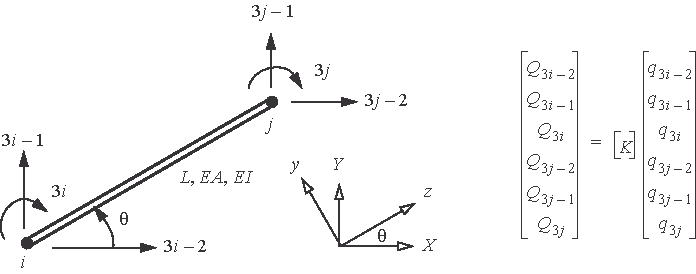
\includegraphics{Figure_16-23.pdf}}
\caption{Frame member with an arbitrary orientation referenced to global coordinate directions.}\label{fig16.23}
\end{figure}

The frame stiffness matrix (\ref{eq16.90}) is symmetric and singular, and the diagonal elements are positive. Equilibrium of the frame member shown in figure~\ref{fig16.23} for each of the six unit displacement states leads to the following relations for the elements of the stiffness matrix.
\begin{itemize}
\item Horizontal equilibrium: $k_{1 j}+k_{4 j}=0$, $j=1,2, \ldots, 6$, which implies row 1 plus row 4 = 0.

\item Vertical equilibrium: $k_{2 j}+k_{5 j}=0$, $j=1,2, \ldots, 6$, which leads to row 2 plus row 5 = 0.

\item Moment equilibrium about joint $i$: $k_{3 j}+(L \sin \theta) k_{4 j}-(L \cos \theta) k_{5 j}+k_{6 j}=0$, $j=1,2, \ldots, 6$, which leads to row 3 plus (L sine($\theta$)) times row 4 minus (L cosine($\theta$)) times row 5 plus row $6 = 0$.
\end{itemize}

\pagebreak

\subsection{Frame stress matrix}\label{sec16.3.3}

The stress matrix for the frame member \textit{i-j} relates the internal axial force $N$, the transverse shear force $V$, and the bending moment $M$ to the generalized joint displacement vector. We can combine the stress matrix for the truss member, eq.~(\ref{eq16.14}), and the stress matrix for the beam member, eq.~(\ref{eq16.44}), if local coordinate direction displacements are employed. With due regard for the joint numbering convention for the frame member relative to the numbering convention of the truss and beam members, the following relationship can be obtained from the stress matrices of the truss and beam members:
\begin{align}\label{eq16.91}
\left[\begin{array}{@{}c@{}}N \\V \\M\end{array}\right]_{i-j}={\underbrace{\left[\begin{array}{@{}cccccc@{}}-E A / L & 0 & 0 & E A / L & 0 & 0 \\0 & -12 E I / L^{3} & 6 E I / L^{2} & 0 & 12 E I / L^{3} & 6 E I / L^{2} \\0 & E I\left(\frac{6}{L^{2}}-\frac{12 z}{L^{3}}\right) & E I\left(-\frac{4}{L}+\frac{6 z}{L^{2}}\right) & 0 & E I\left(-\frac{6}{L^{2}}+\frac{12 z}{L^{3}}\right) & E I\left(-\frac{2}{L}+\frac{6 z}{L^{2}}\right)\end{array}\right]}_{[\bar{S}(z)]_{i-j}}}_{\raisebox{1.4pc}{\small $i{-}j$}}\left[\begin{array}{@{}c@{}}\bar{q}_{3 i-2} \\\bar{q}_{3 i-1} \\\bar{q}_{3 i} \\\bar{q}_{3 j-2} \\\bar{q}_{3 j-1} \\\bar{q}_{3 j}\end{array}\right].
\end{align}
Recall that the axial coordinate $z$ is a local coordinate in the frame element, which is zero at the beginning joint $i$ and equal to the length \textit{L} of the frame element at end joint $j$. The 3X6 stress matrix $[\bar{S}(z)]_{i-j}$ (\ref{eq16.91}) is referenced to the generalized displacement vector in local coordinate directions. The stress matrix in terms of the generalized displacement vector in global coordinate directions is obtained by substituting (\ref{eq16.84}) for the displacement vector in eq.~(\ref{eq16.91}) to get
\begin{align}\label{eq16.92}
\left[\begin{array}{@{}c@{}}N \\V \\M\end{array}\right]_{i-j}=[\bar{S}(z)]_{i-j}[T]_{i-j}\left[\begin{array}{@{}c@{}}q_{3 i-2} \\q_{3 i-1} \\q_{3 i} \\q_{3 j-2} \\q_{3 j-1} \\q_{3 j}\end{array}\right]=[S(z)]_{i-j}\left[\begin{array}{@{}c@{}}q_{3 i-2} \\q_{3 i-1} \\q_{3 i} \\q_{3 j-2} \\q_{3 j-1} \\q_{3 j}\end{array}\right] \quad 0 \leq z \leq L,
\end{align}
where
\begin{align*}
[S(z)]_{i-j}&=\left[\begin{array}{@{}cccc@{}}-E A / L & 0 & 0 & E A / L \\0 & -12 E I / L^{3} & 6 E I / L^{2} & 0 \\0 & E I\left(\frac{6}{L^{2}}-\frac{12 z}{L^{3}}\right) & E I\left(-\frac{4}{L}+\frac{6 z}{L^{2}}\right) & 0\end{array}\right.\left.\begin{array}{@{}ccc@{}}0 & 0 \\12 E I / L^{3} & 6 E I / L^{2} \\E I\left(-\frac{6}{L^{2}}+\frac{12 z}{L^{3}}\right) & E I\left(-\frac{2}{L}+\frac{6 z}{L^{2}}\right)\end{array}\right] \\
&\quad\hspace*{-1.4pt}\left[\begin{array}{@{}cccccc@{}}c & s & 0 & 0 & 0 & 0 \\-s & c & 0 & 0 & 0 & 0 \\0 & 0 & 1 & 0 & 0 & 0 \\0 & 0 & 0 & c & s & 0 \\0 & 0 & 0 & -s & c & 0 \\0 & 0 & 0 & 0 & 0 & 1\end{array}\right].
\end{align*}
Perform the matrix multiplication in the last equation to find
\begin{align}
[S(z)]_{i-j} &=\left[\begin{array}{@{}ccc@{}}-c E A / L & -s E A / L & 0 \\
s 12 E I / L^{3} & -c 12 E I / L^{3} & 6 E I / L^{2} \\
-E I s\left(\frac{6}{L^{2}}-\frac{12 z}{L^{3}}\right) & E I c\left(\frac{6}{L^{2}}-\frac{12 z}{L^{3}}\right) & E I\left(-\frac{4}{L}+\frac{6 z}{L^{2}}\right)\end{array}\right. \nonumber \\
&\qquad\left.\begin{array}{@{}ccc@{}}c E A / L & s E A / L & 0 \\-s 12 E I / L^{3} & c 12 E I / L^{3} & 6 E I / L^{2} \\-E I s\left(-\frac{6}{L^{2}}+\frac{12 z}{L^{3}}\right) & E I c\left(-\frac{6}{L^{2}}+\frac{12 z}{L^{3}}\right) & E I\left(-\frac{2}{L}+\frac{6 z}{L^{2}}\right)\end{array}\right]_{i-j}. \label{eq16.93}
\end{align}
The 3X6 stress matrix $[S(z)]_{i-j}$, $0 \leq z \leq L$, for the frame member relates the internal actions in local coordinate directions $z$ and $y$ to the generalized displacement vector in global coordinate directions.

\vspace*{-1pc}

\begin{example}[Portal frame]\label{ex16.8}The coplanar rectangular frame shown in figure~\ref{fig16.24} consists of three members: 1-2, 2-3, and 3-4. Joints1 and 4 are restrained against displacement and rotation. At joint 2 there is a rigid connection between members 1-2 and 2-3, and at joint 3 there is a rigid connection between members 2-3 and 3-4. Joints 2 and 3 are moveable, and the generalized displacement vector for these joints is $\left\{q_{\alpha}\right\}=\left[\begin{array}{@{}l@{\;}l@{\;}l@{\;}l@{\;}l@{\;}l@{}}q_{4} & q_{5} & q_{6} & q_{7} & q_{8} & q_{9}\end{array}\right]^{T}$. Each member has a cross-sectional area $A=1,500 \mathrm{~mm}^{2}$, second area moment $I=2.8 \times 10^{6} \mathrm{~mm}^{4}$, and the same modulus of elasticity $E=70 \times 10^{3} \mathrm{~N}/ \mathrm{mm}^{2}$. The direction cosines for member 1-2 are $(c, s)=(0,1)$, for member 2-3 $(c, s)=(1,0)$, and for member 3-4 $(c, s)=(0,-1)$. Determine the generalized displacements of the movable joints 2 and 3, and the bending moment in each member.

\begin{figure}[!h]
\vspace*{-2pc}
\centerline{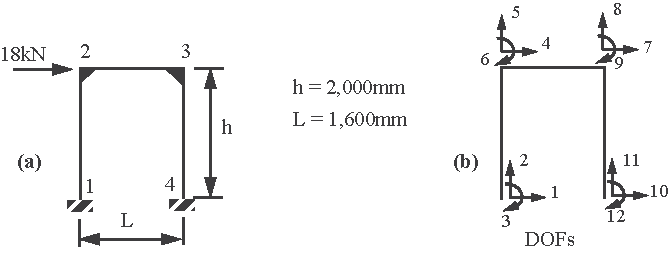
\includegraphics{Figure_16-24.pdf}}
\caption{(a) Portal frame. (b) Degree of freedom numbering.}\label{fig16.24}
\vspace*{-1.2pc}
\end{figure}

The stiffness\enlargethispage{0\baselineskip} matrix (\ref{eq16.90}) for each member including only the generalized displacements of joints 2 and 3 are as follows:\vspace*{-1.8pc}
\begin{align}
\left[K_{1-2}\right]&=
\begin{array}{@{}c@{}}
{\arraycolsep=16pt
\begin{array}{@{}ccc@{}}\hspace*{-1pc}q_{4} & q_{5} & q_{6}\end{array}} \\[3pt]\left[\begin{array}{@{}ccc@{}}(12 E I) / h^{3} & 0 & (-6 E I) / h^{2} \\0 & (E A) / h & 0 \\(-6 E I) / h^{2} & 0 & (4 E I) / h\end{array}\right]\end{array}=\begin{array}{@{}c@{}}
{\arraycolsep=16pt\begin{array}{@{}ccc@{}}q_{4} & q & q_{6}\end{array}} \\[3pt]\left[\begin{array}{@{}ccc@{}}294 & 0 & -294{,}000 \\0 & 52{,}500 & 0 \\-294{,}000 & 0 & 3.92 \times 10^{8}\end{array}\right]\end{array},\nonumber\\
\left[K_{2-3}\right]&=\begin{array}{@{}c@{}}
{\arraycolsep=22pt\begin{array}{@{}cccccc@{}}
\hspace*{-1pc}q_4 & q_5 & q_6 & q_7 & q_8 & q_9
\end{array}}\\[3pt]
\left[\begin{array}{@{}cccccc@{}}(E A) / L & 0 & 0 &(-E A) / L & 0 & 0 \\0 & (12 E I) / L^{3} & (-6 E I) / L^{2} &0 & (-12 E I) / L^{3} & (-6 E I) / L^{2} \\0 & (-6 E I) / L^{2} & (4 E I) / L &0 & (6 E I) / L^{2} & (2 E I) / L \\
(-E A) / L & 0 & 0 &(E A) / L & 0 & 0\\
0 & (-12 E I) / L^{3} & (6 E I) / L^{2} &0 & (12 E I) / L^{3} & (6 E I) / L^{2} \\
0 & (-6 E I) / L^{2} & (2 E I) / L &0 & (6 E I) / L^{2} & (4 E I) / L
\end{array}\right]\end{array},\label{eq16.8a}\tag{a} \\
\left[K_{2-3}\right]&=
\begin{array}{@{}c@{}}
{\arraycolsep=20pt\begin{array}{@{}cccccc@{}}
q_4 & q_5 & q_6 & q_7 & q_8 & q_9
\end{array}}\\[6pt]
\left[\begin{array}{@{}cccccc@{}}65{,}625 & 0 &0&-65{,}625 & 0 & 0 \\
0 & 574.219 & -459{,}375 &0 & -574.219 & -459{,}375\\
0& -459{,}375 &4.9 \times 10^{8} &0 & 459{,}375 & 2.45 \times 10^{8} \\
-65{,}625 & 0 &0  & 65{,}625 & 0 & 0 \\
0 & -574.219  &459{,}375 & 0 & 574.219 & 459,375 \\
0&-459{,}375 & 2.45 \times 10^{8} & 0 & 459{,}375 & 4.9 \times 10^{8}\end{array}\right]\end{array}\mbox{, and}\label{eq16.8b}\tag{b} \displaybreak\\
\hspace*{2pc}\left[K_{3-4}\right]&=
\begin{array}{@{}c@{}}
{\arraycolsep=16pt
\begin{array}{@{}ccc@{}}q_{7} & q_{8} & q_{9}\end{array}} \\[6pt]
\left[\begin{array}{@{}ccc@{}}(12 E I) / h^{3} & 0 & (6 E I) / h^{2} \\0 & (E A) / h & 0 \\(6 E I) / h^{2} & 0 & (4 E I) / h\end{array}\right]\end{array}=
\begin{array}{@{}c@{}}
{\arraycolsep=16pt
\begin{array}{@{}ccc@{}}q_{7} & q_{8} & q_{9}\end{array}} \\[6pt]
\left[\begin{array}{@{}ccc@{}}294 & 0 & 294,000 \\0 & 52,500 & 0 \\294,000 & 0 & 3.92 \times 10^{8}\end{array}\right]\end{array}.\label{eq16.8c}\tag{c}
\end{align}
The restrained structural stiffness matrix is obtained by the sum of the member stiffness matrices in eqs. (\textbf{\ref{eq16.8a}}), (\textbf{\ref{eq16.8b}}), and (\textbf{\ref{eq16.8c}}) with due regard to the location of the matrix elements from the individual members to their place in the restrained stiffness matrix. The result is
\begin{align}\label{eq16.8d}\tag{d}
\left[K_{\alpha \alpha}\right]=\begin{array}{@{}c@{}}
{\arraycolsep=20pt\begin{array}{@{}cccccc@{}}
q_4 & q_5 & q_6 & q_7 & q_8 & q_9
\end{array}}\\[6pt]
\left[\begin{array}{@{}cccccc@{}}65,919 & 0 & -294,000 & -65,625 & 0 & 0 \\0 & 53,074.2 & -459,375 & 0 & -574.219 & -459,375 \\-294,000 & -459,375 & 8.82 \times 10^{8} & 0 & 459,375 & 2.45 \times 10^{8} \\-65,625 & 0 & 0 & 65,919 & 0 & -294,000 \\0 & -574.219 & 459,375 & 0 & 53,074.2 & 459,375 \\0 & -459,375 & 2.45 \times 10^{8} & -294,000 & 459,375 & 8.82 \times 10^{8}\end{array}\right]\end{array}.
\end{align}
The prescribed external load vector is $\left\{Q_{\alpha}\right\}=\left[\begin{array}{@{}llllll@{}}
Q_{4} & Q_{5} & Q_{6} & Q_{7} & Q_{8} & Q_{9}\end{array}\right]^{T}=\left[\begin{array}{@{}l@{\;\;\,\,\,}l@{\;\;\,\,\,}l@{\;\;\,\,\,}l@{\;\;\,\,\,}l@{\;\;\,\,\,}l@{}}18,000 \mathrm{~N} & 0 & 0 & 0 & 0 & 0\end{array}\right]^{T}$,\break and the matrix equation to determine the generalized displacements is $\left\{Q_{\alpha}\right\}=\left[K_{\alpha \alpha}\right]\left\{q_{\alpha}\right\}$. The solution for the generalized displacements from the latter equation is
\begin{align}\label{eq16.8e}\tag{e}
\begin{split}
q_{4}=41.6931 \mathrm{~mm} \quad q_{5}=0.18859 \mathrm{~mm} \quad q_{6}=0.0110439\, \mathrm{rad} \text {. }\\
q_{7}=41.5561 \mathrm{~mm} \quad q_{8}=-0.18859 \mathrm{~mm} \quad q_{9}=0.0109807\, \mathrm{rad}
\end{split}.
\end{align}
The bending moment in member 1-2 is determined from its stress matrix (\ref{eq16.93}) and the generalized displacement vector for the member. Reading the third row of the stress matrix determines the bending moment as
\begin{align}\label{eq16.8f}\tag{f}
(M_{x})_{1-2}=\left[-E I(6 / h^{2}-12 z / h^{3}) 0\ E I(-4 / h+6 z / h^{2})-E I(-6 / h^{2}+12 z / h^{3}) 0\ E I(-2 / h+6 z / h^{2})\right]\left\{q_{1-2}\right\},
\end{align}
where $\left\{q_{1-2}\right\}=\left[\begin{array}{@{}llllll@{}}0 & 0 & 0 & q_{4} & q_{5} & q_{6}\end{array}\right]^{T}$. Numerical evaluation results in
\begin{align}
\left(M_{x}\right)_{1-2}=(294,000-294 . z) q_{4}+(-1.96 \times 10^{8}+294,000 z) q_{6} &=1.00931 \times 10^{7}-9,010.84 z \nonumber\\
&\quad 0 \leq z \leq 2,000 \mathrm{~mm}.\label{eq16.8g}\tag{g}
\end{align}
Following the same procedure for members 2-3 and 3-4 we find
\begin{align}
\left(M_{x}\right)_{2-3} &=(459,375-574.219 {z}) q_{5}+(-4.9 \times 10^{8}+459,375 {z}) q_{6}+(-459,375+574.219 {z}) q_{8} \nonumber\\
&\quad +(-2.45 \times 10^{8}+459,375 {z}) q_{9}=-7.92854 \times 10^{6}+9,900.99 {z} \quad 0 \leq {z} \leq 1,600 \mathrm{~mm}\mbox{, and}\label{eq16.8h}\tag{h}\\
\hspace*{-4pt}\left(M_{x}\right)_{3-4} &=(294,000-294 {z}) q_{7}+(-3.92 \times 10^{8}+294,000 {z}) q_{9}=7.91305 \times 10^{6}-8,989.16 {z}, 0 \leq {z} \leq 2,000 \mathrm{~mm}.\label{eq16.8i}\tag{i}
\end{align}
The bending moment in each member is plotted with respect to the axial coordinate in figure~\ref{fig16.25}. The bending moment distribution is linear in each member and it passes through zero as it changes sign.
\end{example}

\processfigure[!h]{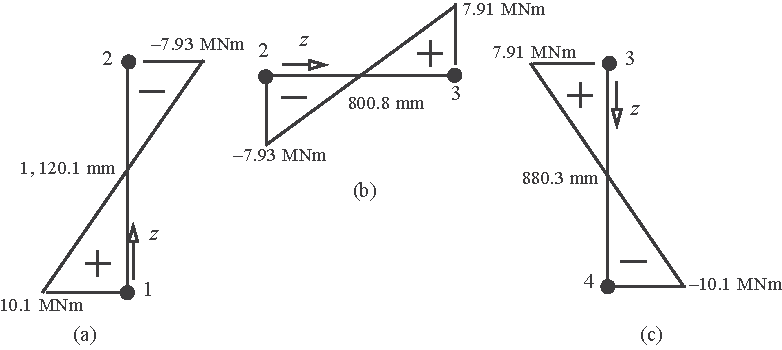
\includegraphics{Figure_16-25.pdf}
}{\caption{Bending moments in the members of the portal frame: (a) member 1-2, (b) member 2-3, (c) member 3-4.}\label{fig16.25}}

\section{Practice exercises}\label{sec16.4}

\begin{exercise}
\begin{enumerate}[\textbf{2.}]
\item[\textbf{1.}] Consider the plane truss restrained against rigid body motion and subject to the loads shown in figure~\ref{fig16.26}(a). Use the degree of freedom numbering convention based on the joint numbering as shown in figure~\ref{fig16.26}(b). All four bars have the same modulus of elasticity $E=10 \times 10^{6}\, \mathrm{psi}$, and the same $A / L$ where the cross-sectional area for bar 1-2 is $0.5 \text { in.}^2$ Solve by hand the computations for the

\processfigure[!h]{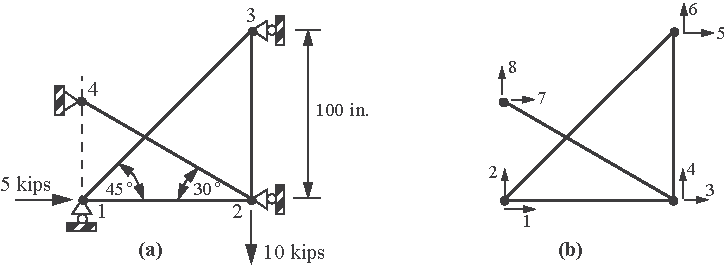
\includegraphics{Figure_16-26.pdf}
}{\caption{(a) Truss with four joints and four members. (b) Degree of freedom numbering.}\label{fig16.26}}

\vspace*{-1.6pc}

\begin{enumerate}[b)]
\item[{\hskip13pt}a)] unrestrained structural stiffness matrix,
\item[{\hskip13pt}b)] restrained structural stiffness matrix, and
\item[{\hskip13pt}c)] unknown joint displacements.
\end{enumerate}

\item[\textbf{2.}] Consider the plane truss consisting of five bars shown in figure~\ref{fig16.27}(a). Each bar has the same extensional stiffness $E A$. Use the degree of freedom numbering convention based on the joint numbers labeled in the figure.

\begin{enumerate}[b)]
\item[{\hskip13pt}a)] Determine the unrestrained structural stiffness matrix.
\item[{\hskip13pt}b)] Joints 1 and 3 are restrained such that $q_{1}=q_{2}=q_{6}=0$, and it is assumed the loads are applied in the\break\hspace*{35pt} remaining degrees of freedom. Determine the submatrix $\left[K_{\beta \alpha}\right]$.
\end{enumerate}

\pagebreak

\item[\textbf{3.}] For the seven-bar truss shown in figure~\ref{fig16.27}(b) all bars have the same value for $E A / L$. The horizontal displacement of joint 5 is prescribed as $q_{9}=1$. All applied forces are zero. Use symmetry to reduce the order of the restrained structural stiffness matrix $\left[K_{\alpha \alpha}\right]$ and then determine the unknown nodal displacements $q_{3}, q_{4}, q_{5}, \text { and } q_{6}$.

\item[\textbf{4.}] In the three-bar truss shown in figure~\ref{fig16.27}(c) the temperature of bar 1-2 is increased $100^{\circ} \mathrm{C}$ above ambient temperature, while bars 1-3 and 1-4 remain at ambient temperature. The bars are made of aluminum alloy with a modulus of elasticity $E=69\, \mathrm{GPa}$ and coefficient of thermal expansion $\alpha=23.6 \times 10^{-6} /{ }^{\circ} C$. The length of each bar $L=250 \mathrm{~mm}$, and the cross-sectional area of each bar $A=400 \mathrm{~mm}^{2}$.

\noindent Determine
\begin{enumerate}[b)]
\item[{\hskip13pt}a)] the 8X1 fixed-end action vector,
\item[{\hskip13pt}b)] the 8X8 unrestrained structural stiffness matrix,
\item[{\hskip13pt}c)] the joint displacements $q_{1}$ and $q_{2}$ of movable joint 1,
\item[{\hskip13pt}d)] the support reactions, and
\item[{\hskip13pt}e)] the bar forces. State if they are in tension or compression.
\end{enumerate}

\processfigure[!h]{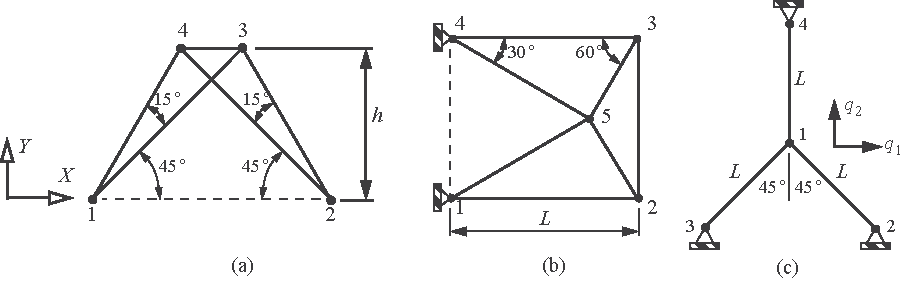
\includegraphics{Figure_16-27.pdf}
}{\caption{Truss configurations. (a) Exercise 2. (b) Exercise 3. (c) Exercise 4.}\label{fig16.27}}

\item[\textbf{5.}] The uniform, multispan beam shown in figure~\ref{fig16.28} is clamped at each end and subject to vertical point loads at joints 2 and 4. Use the joint numbers indicated in the figure, and the degree of freedom numbering convention associated with the joint numbers.

\processfigure[!h]{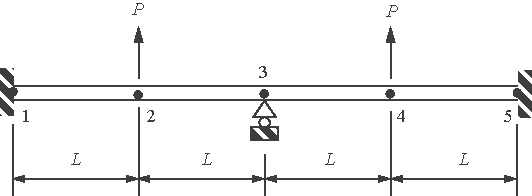
\includegraphics{Figure_16-28.pdf}
}{\caption{Multispan beam.}\label{fig16.28}}

\begin{enumerate}[b)]
\item[{\hskip13pt}a)] Use symmetry to reduce the problem size and compute the joint displacement vector in terms of \textit{P}, \textit{L}, and \textit{EI}.
\item[{\hskip13pt}b)] Determine the shear force and bending moment distributions in each span in terms of \textit{P} and \textit{L}. Sketch the shear force and bending moment diagrams.
\item[{\hskip13pt}c)] Determine the support reactions.
\end{enumerate}

\item[\textbf{6.}] The flexural stiffness of the uniform beam shown in figure~\ref{fig16.29} is $E l$, and it has a of length 2\textit{L}. It is supported by linear elastic springs at each end, each with a stiffness $k=6 E I / L^{3}$. It is subject to the linearly varying distributed load whose intensity is $f_{y 1}$ at midspan.

\processfigure[!h]{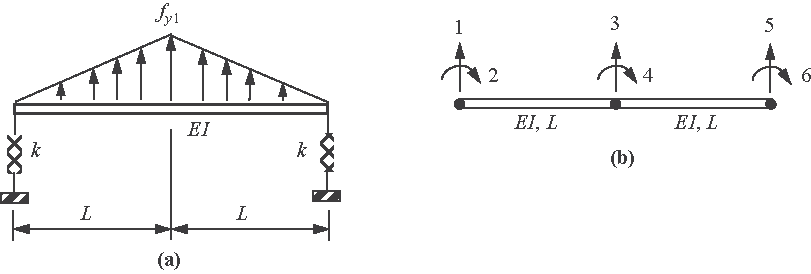
\includegraphics{Figure_16-29.pdf}
}{\caption{(a) Beam with spring supports. (b) Degree of freedom numbering.}\label{fig16.29}}

Use two members to model the beam, and use the degrees of freedom (DOFs) numbering shown in the figure.

\begin{enumerate}[b)]
\item[{\hskip13pt}a)] Use symmetry about the vertical centerline and determine the restrained structural stiffness matrix in\break\hspace*{35pt} DOFs 1, 2, and 3, and in terms of parameters $E I$ and $L$.
\item[{\hskip13pt}b)] Determine the 6X1 fixed-end action vector $\left\{Q^{0}\right\}$ in terms of $f_{y 1}$ and $L$.
\item[{\hskip13pt}c)] Solve for the unknown joint displacement vector $\left[\begin{array}{@{}llllll@{}}q_{1} & q_{2} & q_{3} & q_{4} & q_{5} & q_{6}\end{array}\right]^{T}$ in terms of $E I$, $L$, and~$f_{y 1}$.
\end{enumerate}

\item[\textbf{7.}] Consider the frame shown in figure~\ref{fig16.30}(a) consisting of a vertical bar 1-2 and a horizontal bar 2-3, which are joined together by a rigid connection at joint 2. The ends of the bars opposite to their common joint are clamped. The horizontal bar 1-2 is subject to a linearly distributed load. The degree of freedom numbering convention is shown in figure~\ref{fig16.30}(b).

\vspace*{-8pt}

\processfigure[!h]{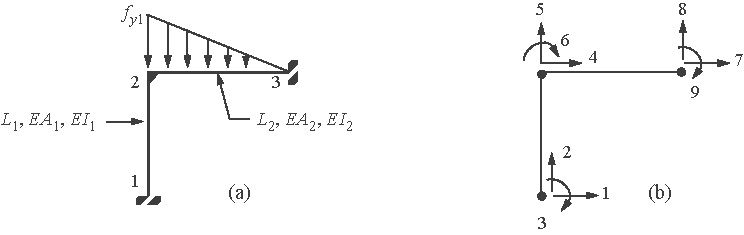
\includegraphics{Figure_16-30.pdf}
}{\caption{(a) Frame configuration. (b) Degree of freedom numbering.}\label{fig16.30}}

\vspace*{-1pc}

\begin{enumerate}[b)]
\item[{\hskip13pt}a)] Determine the restrained structural stiffness matrix $\left[K_{\alpha \alpha}\right]$.
\item[{\hskip13pt}b)] Determine the 9X1 fixed-end action vector $\left\{Q^{0}\right\}$.
\end{enumerate}

\item[\textbf{8.}] Consider the model of a strut-braced wing spar shown in figure~\ref{fig16.31} subject to the span-wise air load approximated as a linearly varying distributed line load. The intensity of the distributed load at the root $f_{y 1}=130.2083\, \mathrm{lb} . / \mathrm{in}$. and the resultant lift acting on the spar is $\frac{1}{2} f_{y_{1}}(32 \times 12)=25,000\, \mathrm{lb}$.

\processfigure[!h]{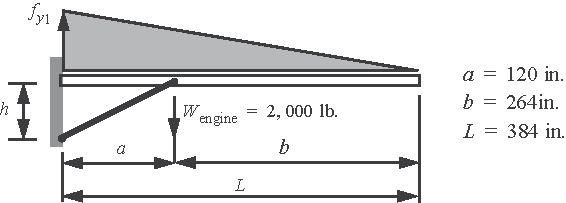
\includegraphics{Figure_16-31.pdf}
}{\caption{Strut-braced wing spar.}\label{fig16.31}}

The spar is clamped at the root and free at the tip, and the strut is pinned-connected to the spar and the support. The matrix structural model consists of three members as shown in figure~\ref{fig16.32}(a). Since the air load bends the spar which in turn stretches the strut, the structure is modeled with a frame member between joints 1 and 2, a beam member between joints 2 and 3. and a truss bar between joints 2 and 4. The degree of freedom numbering convention is shown in figure~\ref{fig16.32}(b).

\processfigure[!h]{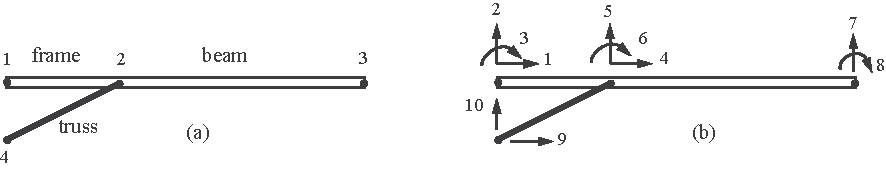
\includegraphics{Figure_16-32.pdf}
}{\caption{(a) Joint numbers for a three-member model. (b) Degrees of freedom.}\label{fig16.32}}

\begin{enumerate}[b)]
\item[{\hskip13pt}a)] Determine the fixed-end action vector $\left\{Q^{0}\right\}$ and its partitions $\left\{Q_{\alpha}^{0}\right\}$ and $\left\{Q_{\beta}^{0}\right\}$. The $\alpha$-indices are 4, 5,\break\hspace*{35pt} 6, 7, and 8, and the $\beta$-indices are 1, 2, 3, 9, and 10.
\item[{\hskip13pt}b)] Additional numerical data are listed in table~\ref{tab16.7}. Determine the unknown nodal displacements.
\end{enumerate}
\end{enumerate}

\begin{table}[!h]%Table 16.7
\processtable{Additional numerical data for the strut-braced wing\label{tab16.7}}
{\tabcolsep=10pt\begin{tabular}{@{}ll@{}}\toprule
$h$, vertical distance from the spar centroid to lower strut support & 60 in.\\
\textit{A}, cross-sectional area of the spar & 23.88 in.$^2$\\
$I_{xx}$, second area moment of the cross section of the spar & 872.716 in.$^4$\\
$A_s$, cross-sectional area of the strut (1.75 in. diameter) & 2.40528 in.$^2$\\
\textit{L}, wing lift & 25,000 lb.\\
\textit{E}, modulus of elasticity for the spar and strut material & $10 \times 10^{6} \mathrm{lb}.{/}\text{in.}{}^{2}$\\\botrule
\end{tabular}}{}
\end{table}

\end{exercise}

\clearemptydoublepage

\end{document} 